%==============================================================================
\chapter{Experimental Evaluations}\label{chap:experiments}
% Avaliação preliminar para a qualificação
%==============================================================================

In this chapter, we present the research questions and hypotheses investigated during the evaluation of our proposal. 
In addition to presenting the experimental design adopted and its conduction.
Section \ref{sec_experiments:preliminaryEval} presents the preliminary evaluation of ERText, which is focused on the assessment of tool features. Section \ref{sec_experiments:finalEval} describe the increments for the next evaluations, carried out until February 2022, which also includes the evaluation of learning features.
In the end, Section \ref{sec_experiments:lessons} draws the chapter's lessons.

%------------------------------------------------------------------------------
\section{Tool Features - Experiment 1} 
\label{sec_experiments:preliminaryEval}
%------------------------------------------------------------------------------

This section presents all the planning, conduction, discussion of the results obtained, threats to validity of the study, and the conclusions regarding the preliminary evaluation carried out to evaluate the first release of a stable prototype of the developed tool.

%######################################################
\subsection{Planning}
\label{ssec_experiments:preliminary_planning}
%######################################################

We carried out this preliminary evaluation from the replication of the experimental protocol performed in a previous study \cite{Lopes:2019}, which aimed to obtain evidence of the comparison from two approaches for modeling relational databases, one graphical and the other textual.
% This preliminary evaluation was carried out from the replication of the experimental protocol performed in a previous study \cite{Lopes:2019} and aims to obtain evidence from the comparison of two approaches for modeling relational databases, one graphical and the other textual.

We specified the following treatments:
\begin{enumerate} [label=\roman*.]
    \item Control treatment: the brModelo tool (graphical approach), and;
    \item Experimental treatment: the ERtext tool (textual approach).
\end{enumerate}
The purpose of this replication is to evaluate the feasibility of using a textual approach to support the teaching-learning process of conceptual modeling relational databases.

\textbf{Context:}
% The context of the experiment is characterized according to four dimensions:
We characterized the context of the experiment according to four dimensions:
\begin{enumerate}[label=\roman*.]
    \item Process: Process: it used an \textit{in-vitro} approach since we performed the tasks under controlled conditions;
    % Process: an \textit{in-vitro} approach was used, since the tasks were performed under controlled conditions.
    %In software engineering, most \textit{in-vitro} experiments are executed in universities or among selected groups of a software development organization \cite{Travassos:2003}.
    \item Subjects: undergrad students in Computer Science (CS) and Software Engineering (SE) programs;
    \item. Reality: the experiment addressed a real problem, \textit{i.e.} the difference in the effort spent of subjects in the conceptual modeling of relational databases; 
    %the artifacts quality produced and the subjects Perceived Usefulness (PU) using both approaches.
    \item Generality: we inserted this evaluation in a specific context, involving database modeling students.
    However, we can replicate the general ideas of this experiment in another set of subjects, approaches, or DSLs that support database designing. 
    % However, the general ideas of this experiment can be replicated in another set of subjects, approaches or DSLs that support database designing.
\end{enumerate}

\textbf{Research Questions (RQs):}
For the controlled experiment results discussion, we decided to formulate four RQs related to the activities performed in the execution of the protocol.
\begin{itemize}
    \item \textbf{RQ1.} Which approach requires the most effort spent on average during the modeling activity?
    \item \textbf{RQ2.} What is the quality level of the models produced using the graphical and textual approaches?
    \item \textbf{RQ3.} What is the subject's perception regarding the Perceived Ease of Use (PEoU) and Perceived Usefulness (PU) of the proposed DSL?
    \item \textbf{RQ4.} What is the subject's assessment concerning the representation of the ER modeling builders supported in the proposed DSL?
\end{itemize}

\textbf{Hypotheses Formulation:} 
% The first two RQs were taken into account. 
We have taken into account the first two RQs. 
Regarding \textbf{RQ1.} 
%the average effort spent required using each approach, our scientific hypotheses are as follows:
% we defined a two-sided hypotheses that measure the average effort spent between textual and graphical approaches during conceptual modeling. State the null (no difference) $H_0 : \mu Time_T = \mu Time_G$ and alternative (significant difference) $H_a : \mu Time_T \neq Time_G$ hypotheses.
\begin{itemize}
    \item \textbf{Null hypothesis:} $H_0 : \mu Time_T = \mu Time_G$: There is no difference in average effort spent measure between textual and graphical approaches during conceptual modeling.
    \item \textbf{Alternative hypothesis:} $H_{1} : \mu Time_T \neq \mu Time_G$: There is a significant difference in average effort spent measure between textual and graphical approaches during conceptual modeling.
\end{itemize}
Regarding \textbf{RQ2.} 
%the modeling effectiveness using each approach, our hypotheses are as follows:
in the same way, we stated two-sided hypotheses that measures the modeling effectiveness between textual and graphical approaches during conceptual modeling.
% The null (no difference) and alternative (significant difference) hypotheses are, respectively: 
% $H_0 : \mu Effectiveness_T = \mu Effectiveness_G$ and 
% $H_a : \mu Effectiveness_T \neq \mu Effectiveness_G$.
\begin{itemize}
    \item \textbf{Null hypothesis:} $H_0 : \mu Effectiveness_T = \mu Effectiveness_G$: There is no difference in effectiveness measures between textual and graphical approaches during conceptual modeling.
    \item \textbf{Alternative hypothesis:} $H_{1} : \mu Effectiveness_T \neq \mu Effectiveness_G$: There is a significant difference in effectiveness measures between textual and graphical approaches during conceptual modeling.
\end{itemize}

\textbf{Statistical Methods:} Unlike the first experiment, this replication included a change in the statistical methods adopted.
Previously, we have used the Shapiro-Wilk normality test and the paired T-test for dependent samples.
This was because the sample was smaller (27) than 30 elements.
However, for samples equal to or greater than this quantity, alternative tests are recommended~\cite{Triola:2018}.

For the effort, we chose the Kolmogorov-Smirnov test to verify normality and the Wilcoxon Signed-Rank test for paired samples to investigate the hypotheses using the time spent metric.
For the effectiveness tests, we have adopted the same statistical methods despite instead of using the time spent metric, another measure was necessary.
Thus, we have performed the F1 calculations, deriving from the harmonic mean of precision and recall metrics, for each model produced in both approaches.
% Thus, we have performed the F1 calculations, which is derived from the harmonic mean of \textit{Precision} and \textit{Recall} metrics, for each of the models produced in both approaches.
The F1 calculation \cite{Derczynski:2016} takes into account variables known as \textit{True Positives}, \textit{False Positives}, and \textit{False Negatives}.
\begin{description}
% \begin{inparadesc}
    \item \textbf{\textit{True Positives (TP)}}: Amount of elements correctly modeled using the approach.
    \item \textbf{\textit{False Positives (FP)}}: Amount of elements incorrectly modeled using the approach. 
    \item \textbf{\textit{False Negatives (FN)}}: Amount of elements not modeled using the approach.
% \end{inparadesc}
\end{description}
From the identification of the variables it is then possible to calculate the \textit{Precision}, \textit{Recall}, and \textit{F1} of each model according to these formulas:
% From the variables identification it is then possible to calculate the \textit{Precision}, \textit{Recall}, and \textit{F1} of each model according to these formulas:
\begin{description}
    \item \textbf{\textit{Precision (PR)}}: $\frac{TP}{TP~+~FP}$ 
    \hfill 
    \textbf{\textit{Recall (RE)}}:$\frac{TP}{TP~+~FN}$
    \hfill
    \textbf{\textit{F1-Score (F1)}}: $\frac{2~*~(PR~*~ RE)}{PR~+~RE}$
\end{description}

\textbf{Experiment Design:} Finally, Figure \ref{fig:designExp} presents the design of the controlled experiment performed. 
We followed the design of one factor with two treatments, where we blocked, balanced, and randomized the subjects, which carried out both treatments, featuring a paired comparison design.

\begin{figure}[!htb]
    \centering
    \caption{Experiment design.}
    \label{fig:designExp}
    

\tikzset{every picture/.style={line width=0.75pt}} %set default line width to 0.75pt        

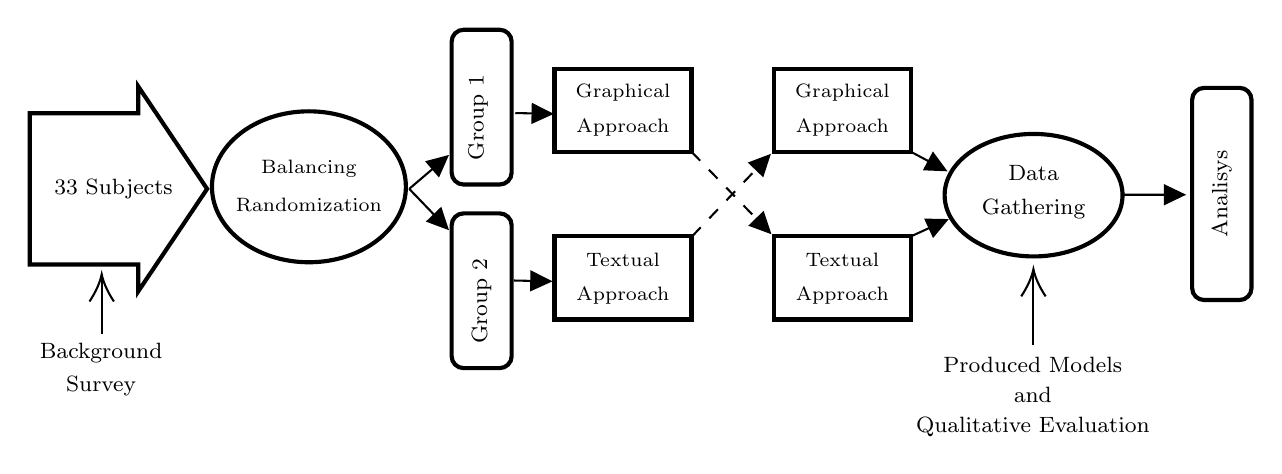
\begin{tikzpicture}[x=0.9pt,y=0.9pt,yscale=-1,xscale=1]
%uncomment if require: \path (0,327); %set diagram left start at 0, and has height of 327


%Shape: Ellipse [id:dp633810982278807] 
\draw  [line width=1.5]  (84.73,72.26) .. controls (84.73,55.52) and (102.16,41.96) .. (123.66,41.96) .. controls (145.16,41.96) and (162.59,55.52) .. (162.59,72.26) .. controls (162.59,88.99) and (145.16,102.56) .. (123.66,102.56) .. controls (102.16,102.56) and (84.73,88.99) .. (84.73,72.26) -- cycle ;



%Shape: Ellipse [id:dp7904221795411808] 
\draw  [line width=1.5]  (378.89,75.63) .. controls (378.89,62.05) and (394.88,51.04) .. (414.61,51.04) .. controls (434.33,51.04) and (450.32,62.05) .. (450.32,75.63) .. controls (450.32,89.21) and (434.33,100.22) .. (414.61,100.22) .. controls (394.88,100.22) and (378.89,89.21) .. (378.89,75.63) -- cycle ;

%Rounded Rect [id:dp5302697683495847] 
\draw  [line width=1.5]  (180.95,87.75) .. controls (180.95,85.09) and (183.11,82.93) .. (185.77,82.93) -- (200.23,82.93) .. controls (202.9,82.93) and (205.06,85.09) .. (205.06,87.75) -- (205.06,140.25) .. controls (205.06,142.91) and (202.9,145.07) .. (200.23,145.07) -- (185.77,145.07) .. controls (183.11,145.07) and (180.95,142.91) .. (180.95,140.25) -- cycle ;
%Rounded Rect [id:dp9616486966995694] 
\draw  [line width=1.5]  (180.95,14.03) .. controls (180.95,11.37) and (183.11,9.21) .. (185.77,9.21) -- (200.23,9.21) .. controls (202.9,9.21) and (205.06,11.37) .. (205.06,14.03) -- (205.06,66.52) .. controls (205.06,69.19) and (202.9,71.35) .. (200.23,71.35) -- (185.77,71.35) .. controls (183.11,71.35) and (180.95,69.19) .. (180.95,66.52) -- cycle ;

%Shape: Rectangle [id:dp03801896284105699] 
\draw  [line width=1.5]  (222.23,24.87) -- (277.28,24.87) -- (277.28,58.21) -- (222.23,58.21) -- cycle ;
%Straight Lines [id:da1799424135415575] 
\draw    (163.93,73.09) -- (177.61,61.43) ;
\draw [shift={(179.89,59.48)}, rotate = 499.54] [fill={rgb, 255:red, 0; green, 0; blue, 0 }  ][line width=0.08]  [draw opacity=0] (8.93,-4.29) -- (0,0) -- (8.93,4.29) -- cycle    ;
%Straight Lines [id:da17029537209985257] 
\draw    (163.93,73.09) -- (177.81,87.53) ;
\draw [shift={(179.89,89.69)}, rotate = 226.13] [fill={rgb, 255:red, 0; green, 0; blue, 0 }  ][line width=0.08]  [draw opacity=0] (8.93,-4.29) -- (0,0) -- (8.93,4.29) -- cycle    ;
%Straight Lines [id:da39402523544663426] 
\draw  [dash pattern={on 4.5pt off 4.5pt}]  (277.5,92.15) -- (307.06,61.21) ;
\draw [shift={(309.13,59.04)}, rotate = 493.69] [fill={rgb, 255:red, 0; green, 0; blue, 0 }  ][line width=0.08]  [draw opacity=0] (8.93,-4.29) -- (0,0) -- (8.93,4.29) -- cycle    ;
%Straight Lines [id:da7992081880522388] 
\draw  [dash pattern={on 4.5pt off 4.5pt}]  (277.28,58.21) -- (307.27,89.16) ;
\draw [shift={(309.35,91.31)}, rotate = 225.9] [fill={rgb, 255:red, 0; green, 0; blue, 0 }  ][line width=0.08]  [draw opacity=0] (8.93,-4.29) -- (0,0) -- (8.93,4.29) -- cycle    ;
%Right Arrow [id:dp3913444800583221] 
\draw  [line width=1.5]  (11.57,42.74) -- (55.14,42.74) -- (55.14,31.99) -- (82.78,73.11) -- (55.14,114.23) -- (55.14,103.49) -- (11.57,103.49) -- cycle ;
%Shape: Rectangle [id:dp003852149638719382] 
\draw  [line width=1.5]  (310.31,24.87) -- (365.36,24.87) -- (365.36,58.21) -- (310.31,58.21) -- cycle ;
%Shape: Rectangle [id:dp0126542660109914] 
\draw  [line width=1.5]  (310.31,92.18) -- (365.36,92.18) -- (365.36,125.52) -- (310.31,125.52) -- cycle ;
%Shape: Rectangle [id:dp4954877903085966] 
\draw  [line width=1.5]  (222.23,92.18) -- (277.28,92.18) -- (277.28,125.52) -- (222.23,125.52) -- cycle ;
%Straight Lines [id:da3442884963113835] 
\draw    (365.36,58.21) -- (377.4,64.63) ;
\draw [shift={(380.04,66.05)}, rotate = 208.07999999999998] [fill={rgb, 255:red, 0; green, 0; blue, 0 }  ][line width=0.08]  [draw opacity=0] (8.93,-4.29) -- (0,0) -- (8.93,4.29) -- cycle    ;
%Straight Lines [id:da6883068419855551] 
\draw    (365.36,92.18) -- (377.84,86.46) ;
\draw [shift={(380.57,85.22)}, rotate = 515.4100000000001] [fill={rgb, 255:red, 0; green, 0; blue, 0 }  ][line width=0.08]  [draw opacity=0] (8.93,-4.29) -- (0,0) -- (8.93,4.29) -- cycle    ;
%Rounded Rect [id:dp5928061300931144] 
\draw  [line width=1.5]  (478.27,37.32) .. controls (478.27,34.68) and (480.41,32.55) .. (483.04,32.55) -- (497.34,32.55) .. controls (499.97,32.55) and (502.1,34.68) .. (502.1,37.32) -- (502.1,112.96) .. controls (502.1,115.59) and (499.97,117.72) .. (497.34,117.72) -- (483.04,117.72) .. controls (480.41,117.72) and (478.27,115.59) .. (478.27,112.96) -- cycle ;

%Straight Lines [id:da6932528701926595] 
\draw    (450.32,75.46) -- (472.85,75.45) ;
\draw [shift={(475.85,75.45)}, rotate = 539.96] [fill={rgb, 255:red, 0; green, 0; blue, 0 }  ][line width=0.08]  [draw opacity=0] (8.93,-4.29) -- (0,0) -- (8.93,4.29) -- cycle    ;
%Straight Lines [id:da7950818392289087] 
\draw    (40.46,131.56) -- (40.46,109.39) ;
\draw [shift={(40.46,107.39)}, rotate = 450] [color={rgb, 255:red, 0; green, 0; blue, 0 }  ][line width=0.75]    (10.93,-4.9) .. controls (6.95,-2.3) and (3.31,-0.67) .. (0,0) .. controls (3.31,0.67) and (6.95,2.3) .. (10.93,4.9)   ;
%Straight Lines [id:da5784112946450906] 
\draw    (414.54,135.73) -- (414.54,107.33) ;
\draw [shift={(414.54,105.33)}, rotate = 450] [color={rgb, 255:red, 0; green, 0; blue, 0 }  ][line width=0.75]    (10.93,-4.9) .. controls (6.95,-2.3) and (3.31,-0.67) .. (0,0) .. controls (3.31,0.67) and (6.95,2.3) .. (10.93,4.9)   ;
%Straight Lines [id:da04489153588175898] 
\draw    (206.5,42.65) -- (218.97,42.92) ;
\draw [shift={(221.97,42.99)}, rotate = 181.23] [fill={rgb, 255:red, 0; green, 0; blue, 0 }  ][line width=0.08]  [draw opacity=0] (8.93,-4.29) -- (0,0) -- (8.93,4.29) -- cycle    ;
%Straight Lines [id:da30869554668079413] 
\draw    (205.97,109.89) -- (218.45,110.16) ;
\draw [shift={(221.44,110.22)}, rotate = 181.23] [fill={rgb, 255:red, 0; green, 0; blue, 0 }  ][line width=0.08]  [draw opacity=0] (8.93,-4.29) -- (0,0) -- (8.93,4.29) -- cycle    ;




% Text Node
\draw (249.75,48.63) node  [font=\scriptsize] [align=left] {Approach};
% Text Node
\draw (249.75,34.46) node  [font=\scriptsize] [align=left] {Graphical};
% Text Node
\draw (490.19,75.14) node  [font=\footnotesize,rotate=-270] [align=left] {Analisys};
% Text Node
\draw (414.31,168.64) node  [font=\footnotesize] [align=left] {Qualitative Evaluation};
% Text Node
\draw (414.31,155.81) node  [font=\footnotesize] [align=left] {and};
% Text Node
\draw (414.31,143.84) node  [font=\footnotesize] [align=left] {Produced Models};
% Text Node
\draw (187.85,136.5) node [anchor=north west][inner sep=0.75pt]  [font=\footnotesize,rotate=-270] [align=left] {Group 2};
% Text Node
\draw (337.84,34.46) node  [font=\scriptsize] [align=left] {Graphical};
% Text Node
\draw (337.84,48.63) node  [font=\scriptsize] [align=left] {Approach};
% Text Node
\draw (249.75,101.76) node  [font=\scriptsize] [align=left] {Textual};
% Text Node
\draw (249.75,115.93) node  [font=\scriptsize] [align=left] {Approach};
% Text Node
\draw (337.84,101.76) node  [font=\scriptsize] [align=left] {Textual};
% Text Node
\draw (337.84,115.93) node  [font=\scriptsize] [align=left] {Approach};
% Text Node
\draw (414.61,66.67) node  [font=\footnotesize] [align=left] {Data};
% Text Node
\draw (414.61,81.26) node  [font=\footnotesize] [align=left] {Gathering};
% Text Node
\draw (40.22,138.89) node  [font=\footnotesize] [align=left] {Background};
% Text Node
\draw (40.22,152.23) node  [font=\footnotesize] [align=left] {Survey};
% Text Node
\draw (123.66,64.96) node  [font=\scriptsize] [align=left] {Balancing};
% Text Node
\draw (123.66,79.56) node  [font=\scriptsize] [align=left] {Randomization};
% Text Node
\draw (186.5,62.78) node [anchor=north west][inner sep=0.75pt]  [font=\footnotesize,rotate=-270] [align=left] {Group 1};
% Text Node
\draw (45.21,73.11) node  [font=\footnotesize] [align=left] {33 Subjects};


\end{tikzpicture}

    % \includegraphics[width=\columnwidth]{images/DesignExperimento.png}
    \fonte{Author.}
\end{figure}

%###########################################################
\subsection{Conduction}
\label{ssec_experiments:preliminary_conduction}
%###########################################################

\textbf{Preparation:} 
Initially, remote meetings were held between the researchers involved to define the planning and the mode of operation that should be adopted, in response to the current scenario of exception due to the worldwide pandemic.
As a result, activities were defined that should be adapted in relation to the first experiment, which was conducted in person.
In order to capture a significant sample for the object of study, it was decided to contact the professors responsible for teaching two courses of different undergraduate courses: Database (SE) and Database I (CS) in the first half of 2021.
% With the initial objectives aligned, the collaborating teachers made the disclosure of profile questionnaires (Google Forms) to the subjects.
Once the initial objectives aligned, the collaborating teachers disclosed the profile questionnaires (Google Forms) to the subjects.

We reused the four (4) instruments from the original experiment. 
The first two were modeling problems with similar levels of complexity, while the last two were qualitative assessments.
We decided that the activities would carry out remotely, respecting the health security protocols required (social distancing). 
For this purpose, we prepared a virtual machine with the tools installed, even as the instruments and supporting materials. 
This virtual machine should be accessed on the university's computers by the subjects using their institutional credentials.
% The four (4) instruments from the original experiment were reused. 
% The first two were modeling problems with similar levels of complexity, while the last two were of qualitative assessment.
% It was decided that the activities would be carried out remotely, respecting the health security protocols required (social distancing). 
% For this purpose, a virtual machine was prepared with the tools installed, as well as the instruments and supporting materials. 
% This virtual machine should be accessed on the university's computers by the subjects using their institutional credentials.

\textbf{Execution:} 
The profile form also served as a term of participation, since the presence in the experiment was voluntary.
With this information, then we have randomized the subjects to define the groups.
% With this information, the subjects were then randomized to define the groups.
We did not find wide discrepancies among the subjects' knowledge levels, demonstrating a homogeneous sample in general.
% We found that there were no major discrepancies between the levels of knowledge of the subjects, demonstrating that there was a homogeneous sample in general.
On the experiment day, the first activity carried out was a brief initial presentation.
Then, the training phase of the participants began.
During this phase, we have presented the two database modeling tools used in the experiment, providing an overview of the operation and answering possible questions that arose.
% During this phase, the two database modeling tools that would be used were presented, providing an overview of the operation and answering possible questions that arose.
The training included the display of videos demonstrating the tools, brModelo and our proposal, respectively.

Then, we start the modeling phase of the proposed problems.
All subjects accessed the virtual machines with the problems provided in PDF documents.
% When starting Instrument 1, all participants were informed with which tool they should develop the solution, thus respecting the groups to which they were part.
When starting Instrument 1, we informed which tool each participant should develop the solution, thus respecting the group to which one was part.
We asked the subjects to write down the start and end times of the tasks for each instrument they performed.
We stipulated no time limit for completion according to the subjects who completed the modeling task. 
We asked them to comply with the guidelines included in the support material for saving the generated artifacts.
% We stipulated no time limit for completion and, according to the subjects completed the modeling task, they were asked to comply with the guidelines included in the support material for saving the generated artifacts.
With the models saved, we informed the subjects that they should move on to the next task described in Instrument 2, although it was necessary to use the reverse approach to the one they had initially used.

At the end of the instruments that contained the modeling problems, we delivered the qualitative assessment instruments.
As the subjects had completed the tasks, then we had thanked and released them.
With the conclusion of the experiment by 33 subjects, we closed the evaluation and we performed the stage of result analysis.

%###########################################################
\subsection{Results Analysis}
\label{ssec_experiments:preliminary_resultAnalysis}
%###########################################################

We have performed all Kolmogorov-Smirnov and Wilcoxon Signed-Rank calculations with the support of the R language and the Gnumeric software. In parallel with the validation of a specialist in the statistics field and the aid of literature \cite{Triola:2018}.
% All Kolmogorov-Smirnov and Wilcoxon Signed-Rank calculations were performed with the support of the R language and the Gnumeric software, in parallel with the validation of a specialist in the field of statistics and the aid of literature \cite{Triola:2018}.

\textbf{Effort:} 
To answer \textbf{RQ1.} 
%regarding the effort to use the approaches, 
% the execution times were extracted from the instruments.
we have extracted the execution times from the instruments.
From the gross amount of the execution times, we have calculated the difference to perform the Kolmogorov-Smirnov normality test.
Because it is a statistical test, this technique has the product of measuring the $p$-value.
For this test, we adopted a significance level of $\alpha$~=~5\%.
It means that the p-value is less than 5\%, then we rejected a hypothesis that the distribution is normal.
% This means that the $p$-value is less than 5\% ($p$ < 0.05), a hypothesis that the distribution is normal should be rejected.

After calculations with the set of time differences, we reached a $p$-value of 0.26218.
As $p$-value > $\alpha$, we do not reject the null hypothesis, thus concluding that the data is normally distributed.
%\textit{i.e.}, 
In other words, the difference between the data sample and the normal distribution is not large enough to be statistically significant.
It is important to note that the higher the $p$-value, the more it supports a null hypothesis.
% In the case of the result obtained, the chance of type 1 error (rejecting a null hypothesis that is correct) is very high, and can be translated into 26.21\% (0.26218).
In the case of the result obtained, the chance of type 1 error (rejecting a correct null hypothesis) is very high and translates into 26.21\% (0.26218).
Once we performed the normality tests on the sample, we carried out the hypothesis test of the average effort regarding \textbf{RQ1.}
In the Wilcoxon Signed-Rank test for dependent samples, we used a significance level of $\alpha$~=~5\%, with which we reached a measure of 0.77948 for the $p$-value.
Because it is a two-tailed test, \textit{i.e.} it includes equality in its null hypothesis, this $p$-value shows not enough evidence to guarantee the rejection of the statement of $H_0: \mu Time_G = \mu Time_T$.
Therefore, we do not reject the null hypothesis that the approaches have no difference in average efforts, once according to the test, this difference is not statistically significant. 
Figure \ref{fig:boxplotTempo1} displays a box-plot with the variation of data observed through these data.

% \begin{figure}[!htb]
%     \centering
%     % \includegraphics[width=.9\columnwidth]{experimentResults/EsforcoBoxplot.pdf}
%     % \begin{tikzpicture}
%   \begin{axis}
%     [
    % boxplot/draw direction=y,
    % xtick={1, 2},
    % ylabel={\footnotesize Time (minutes)},
    % xticklabels={{\footnotesize Graphical Treatment}, {\footnotesize Textual Treatment}},
    % height= 5cm
%     ]
%     \addplot+[fill=olive, fill opacity=0.7, draw=black,
%     boxplot prepared={
%       median=25.00,
%       upper quartile=28.00,
%       lower quartile=21.00,
%       upper whisker=60.00,
%       lower whisker=12.00
%     },
%     ] coordinates {};
%     \addplot+[fill=teal, fill opacity=0.7, draw=black,
%     boxplot prepared={
%       median=33.00,
%       upper quartile=43.00,
%       lower quartile=27.00,
%       upper whisker=60.00,
%       lower whisker=15.00
%     },
%     ] coordinates {};
%   \end{axis}
% \end{tikzpicture}

\begin{filecontents*}{data.csv}
11,12,14,15,17,17,19,19,20,21,30,30,32,32,32,33,35,35,35,37,39,42,43,45,45,46,48,50,51,51,51,60,60
17,20,21,21,23,23,24,26,26,26,27,27,30,31,31,34,36,38,38,38,39,40,40,40,40,44,46,47,48,49,50,52,60
\end{filecontents*}

\begin{tikzpicture}
    \pgfplotstableread[col sep=comma]{data.csv}\csvdata
    % Boxplot groups columns, but we want rows
    \pgfplotstabletranspose\datatransposed{\csvdata} 
    \begin{axis}[
        boxplot/draw direction=y,
        xtick={1, 2},
        ylabel={\scriptsize Time (minutes)},
        xticklabels={{\scriptsize Graphical Treatment}, {\scriptsize Textual Treatment}},
        height=7cm,
        width=10cm,
        % boxplot/draw direction = y,
        % axis x line* = bottom,
        % axis y line = left,
        % enlarge y limits,
        ymajorgrids,
        % xtick = {1, 2},
        % xticklabel style = {align=center, font=\small},
        % xticklabels = {Graphical Treatment, Textual Treatment},
        % ylabel = {Time (minutes)},
        ytick = {15, 30, 45, 60},
        yticklabel style = {font=\scriptsize}
    ]
        \foreach \n in {1,...,2} {
            \addplot+[boxplot, fill, fill opacity=0.4, draw=black] table[y index=\n] {\datatransposed};
        }
    \end{axis}
\end{tikzpicture}


%     % \includesvg[width=.7\columnwidth]{figures/Effort}
%     \caption{Box-plot - Effort per treatments.}
%     \label{fig:boxplotTempo1}
% \end{figure}

\textbf{Effectiveness:} 
% To answer \textbf{RQ2.} regarding the effectiveness of the use of approaches
To answer \textbf{RQ2.} regarding the approaches' use effectiveness, we evaluated the artifacts produced by the subjects according to the established reference models\footnote{Available at: \url{https://doi.org/10.5281/zenodo.5454378}}. 
% In this evaluation, we used F1 from the area of pattern recognition and information retrieval. 
In this evaluation, we used F1 from the pattern recognition and information retrieval areas. 
F1 represents the combination of the observed accuracy and recallability of a result concerning a reference.
By definition, this combination refers to Precision and Recall metrics, where Precision is the proportion of recovered instances that are relevant and Recall is the proportion of relevant instances that are recovered.

In addition, we performed the Kolmogorov-Smirnov normality test to F1 for each model. 
After calculations with the set of differences in F1 for each model, we reached a $p$-value of 0.45459.
With this test result, the chance of type 1 error (rejecting a correct null hypothesis) can be very high, and can be translated into 45.45\% (0.45459).
As the $p$-value > $\alpha$, we do not reject the null hypothesis, thus realizing that the data is normally distributed
%, \textit{i.e.} the difference between the data sample and the normal distribution is not large enough to be statistically significant.
After the sample was tested for normality, we tested the second hypothesis defined in this experiment.
This time, in the Wilcoxon Signed-Rank test for dependent samples, we used again a significance level of $\alpha$~=~5\%, with which we reached a measure of 0.00197 for the $p$-value.
% By the original statement including an equality, also characterizing this test as two-tailed, it was concluded that the calculated $p$-value demonstrates that there is enough evidence to guarantee the rejection of the statement of the original null hypothesis, denoted as $H_0: \mu Effectiveness_G = \mu Effectiveness_T$.
By the original statement including equality, also characterizing this test as two-tailed, we concluded that the calculated $p$-value demonstrated enough evidence to guarantee the statement rejection of the original null hypothesis, denoted as $H_0: \mu Effectiveness_G = \mu Effectiveness_T$.
% Therefore, we reject the null hypothesis that the approaches have equal effectiveness, because according to the statistical test, the average difference of F1 among treatments is statistically significant.
Therefore, we rejected the null hypothesis that the approaches have equal effectiveness, once according to the statistical test, the average difference of F1 among treatments is statistically significant.
Table \ref{tab:ResultsModelosGeral} shows average measures of the evaluated values and also provides the possibility to carry out a dispersion analysis.
Based on these data, it was possible to verify that the textual approach has an advantage on average.

\rowcolors{1}{gray!15}{white}
\begin{table}[!htb]
    \caption{Measures of the conceptual data models produced in the experiment.}
    \label{tab:ResultsModelosGeral}
    \centering
    % \scriptsize
    \tiny
    \begin{tabular}{l|ccccc|ccccc}%{l|ccccc|ccccc}
    \bottomrule
    \rowcolor[HTML]{C0C0C0}
    \multicolumn{1}{l}{} &
    \multicolumn{5}{c|}{\textbf{Graphical Treatment}} &
    \multicolumn{5}{c}{\textbf{Textual Treatment}}
    \\ 
    \hline
    \rowcolor[HTML]{C0C0C0}
    \textbf{Measure} & \textbf{MI} & \textbf{RI} & \textbf{P(\%)} & \textbf{R(\%)} & \textbf{F1(\%)} &
    \textbf{MI} & \textbf{RI} & \textbf{P(\%)} & \textbf{R(\%)} & \textbf{F1(\%)}
    \\
    \hline
Maximum	&	47.00	&	36.00	&	96.67	&	92.31	&	88.00	&	56.00	&	46.00	&	97.22	&	97.87	&	91.36	\\
3\textdegree Quartile	&	31.00	&	28.00	&	92.31	&	63.04	&	76.32	&	34.00	&	31.00	&	94.74	&	75.00	&	82.86	\\
Median	&	26.00	&	24.00	&	88.89	&	56.41	&	68.85	&	30.00	&	29.00	&	90.63	&	65.96	&	74.63	\\
Average	&	27.52	&	24.12	&	87.69	&	57.96	&	69.13	&	30.88	&	27.45	&	89.49	&	63.65	&	73.16	\\
1\textdegree Quartile	&	23.00	&	20.00	&	84.21	&	50.00	&	62.50	&	26.00	&	23.00	&	87.88	&	51.06	&	63.01	\\
Minimum	&	18.00	&	16.00	&	72.73	&	41.03	&	52.46	&	19.00	&	15.00	&	72.73	&	31.91	&	45.45	\\
Variance	&	35.58	&	28.65	&	42.87	&	143.35	&	78.93	&	63.32	&	39.76	&	42.59	&	259.85	&	133.58	\\
SD &	5.97	&	5.35	&	6.55	&	11.97	&	8.88	&	7.96	&	6.31	&	6.53	&	16.12	&	11.56	\\
    \toprule
\end{tabular}
\begin{tablenotes}
    \scriptsize
    \centering
    \item \textit{Legend: MI = Modeled Items; RI = Relevant Items; P = Precision; R = Recall; F1 = F1-Score; SD = Standard Deviation.}
\end{tablenotes}
\fonte{Author.}
\end{table}

Figure \ref{fig:boxplotMedidaF1} box-plot graph displays the F1-Score for each treatment applied. 
Based on this graph, it is possible to verify the result obtained in the hypothesis test because the data dispersion does present a significant difference between the approaches.


\begin{figure}[!htb]
        \centering
        \caption{Box-plot - Effort per treatments.}
        \label{fig:boxplotTempo1}
        % \begin{tikzpicture}
%   \begin{axis}
%     [
    % boxplot/draw direction=y,
    % xtick={1, 2},
    % ylabel={\footnotesize Time (minutes)},
    % xticklabels={{\footnotesize Graphical Treatment}, {\footnotesize Textual Treatment}},
    % height= 5cm
%     ]
%     \addplot+[fill=olive, fill opacity=0.7, draw=black,
%     boxplot prepared={
%       median=25.00,
%       upper quartile=28.00,
%       lower quartile=21.00,
%       upper whisker=60.00,
%       lower whisker=12.00
%     },
%     ] coordinates {};
%     \addplot+[fill=teal, fill opacity=0.7, draw=black,
%     boxplot prepared={
%       median=33.00,
%       upper quartile=43.00,
%       lower quartile=27.00,
%       upper whisker=60.00,
%       lower whisker=15.00
%     },
%     ] coordinates {};
%   \end{axis}
% \end{tikzpicture}

\begin{filecontents*}{data.csv}
11,12,14,15,17,17,19,19,20,21,30,30,32,32,32,33,35,35,35,37,39,42,43,45,45,46,48,50,51,51,51,60,60
17,20,21,21,23,23,24,26,26,26,27,27,30,31,31,34,36,38,38,38,39,40,40,40,40,44,46,47,48,49,50,52,60
\end{filecontents*}

\begin{tikzpicture}
    \pgfplotstableread[col sep=comma]{data.csv}\csvdata
    % Boxplot groups columns, but we want rows
    \pgfplotstabletranspose\datatransposed{\csvdata} 
    \begin{axis}[
        boxplot/draw direction=y,
        xtick={1, 2},
        ylabel={\scriptsize Time (minutes)},
        xticklabels={{\scriptsize Graphical Treatment}, {\scriptsize Textual Treatment}},
        height=7cm,
        width=10cm,
        % boxplot/draw direction = y,
        % axis x line* = bottom,
        % axis y line = left,
        % enlarge y limits,
        ymajorgrids,
        % xtick = {1, 2},
        % xticklabel style = {align=center, font=\small},
        % xticklabels = {Graphical Treatment, Textual Treatment},
        % ylabel = {Time (minutes)},
        ytick = {15, 30, 45, 60},
        yticklabel style = {font=\scriptsize}
    ]
        \foreach \n in {1,...,2} {
            \addplot+[boxplot, fill, fill opacity=0.4, draw=black] table[y index=\n] {\datatransposed};
        }
    \end{axis}
\end{tikzpicture}


        \fonte{Author.}
\end{figure}


\begin{figure}[!htb]
        \centering
        \caption{Box-plot - F1 per treatments.}
        \label{fig:boxplotMedidaF1}
        \include{img/boxplotMedidaF1}
        \fonte{Author.}
\end{figure}

% \begin{figure}[!htb]
%     \centering
%     % \includegraphics[width=.9\columnwidth]{experimentResults/EfetividadeBoxplot.pdf}
%     \include{figures/boxplotMedidaF1}
%     % \includesvg[width=.7\columnwidth]{figures/F-Score}
%     \caption{Box-plot - F1 per treatments.}
%     \label{fig:boxplotMedidaF1}
% \end{figure}

\textbf{Qualitative Evaluation:} 
We took place with the analysis of the two instruments applied after the modeling tasks.
We have used the first instrument according to the TAM model \cite{Davis:1989,Persico:2014} to answer the \textbf{RQ3.} regarding the PEoU and PU.
% The first was used to respond to \textbf{RQ3.} regarding the PEoU and PU of treatments, according to the TAM model \cite{Davis:1989,Persico:2014}. 
It occurred through the selection of quality attributes described in ISO/IEC 25010.
% For this, we established a Likert scale from one to six points to measure the level of agreement of the subjects in the face of the statements exposed in the form.
For this, we established a Likert scale from one to six points to measure the subjects' agreement level in the face of the statements exposed in the form.
% This scale served to measure the level of agreement of the subjects in the face of the statements exposed in the form.
We have chosen an even number of alternatives to avoid possible neutral responses.
% Thus, the 7 quality attributes are grouped into three (3) categories being defined as follows:
Thus, we grouped the seven (7) quality attributes into three (3) defined categories as follows:

\begin{itemize}
% \begin{inparaenum}
    \item \textbf{Functionality} 
        \begin{itemize}
            \item \textit{Conformity}: ability level to which the software achieves specified goals with functional completeness, correctness, and appropriateness related to their functionalities.
        \end{itemize}
    \item \textbf{Usability}
        \begin{itemize}
            %Appropriateness recognisability
            \item \textit{Understandability}: ability level to which users can recognize whether the software is appropriate for their needs; 
            \item \textit{Learnability}: ability level to which the software enables the user to learn how to use it with effectiveness, efficiency in emergencies;
            \item \textit{Operability}: ability level to which the software is easy to operate, control, and appropriate to use.
        \end{itemize}
    \item \textbf{Quality in Use}
        \begin{itemize}
            \item \textit{Quality in Use}: ability level to which the software to achieve specified goals with effectiveness and efficiency with their users in specific contexts of use;
            % Performance Efficiency
            \item \textit{Productivity}: ability level to which the software to achieve specified goals with time-behavior, resources utilization and capacity, when performing its functions, meet requirements;
            \item \textit{Satisfaction}: ability level to which the software to achieve specified goals with usefulness, trust, pleasure and comfort with their users in specific contexts of use.
        \end{itemize}
        % \end{inparadesc}
% \end{inparaenum}
\end{itemize}

After summarizing the results, we observed a good acceptance by the subjects for the ERtext tool developed in this work.
Figure \ref{fig:inst3GERALExp} synthesizes the responses received for each quality attribute, showing a certain degree of similarity in the subjects' perception during the application of the treatments.
% A point that can be emphasized is the set of positive responses concerning the \textit{Productivity} and \textit{Operability} since in the hypothesis test related to the effort, the treatments demonstrated a similar need for execution time.
It is worth emphasizing a point that is the positive responses set concerning the \textit{Productivity} and \textit{Operability} since the hypothesis test related to the effort the treatments demonstrated a similar need for execution time.
According to the evaluations received, the most evident disadvantages of ERtext are manifested mainly concerning \textit{Understandability} and \textit{Learnability} quality attributes.

\begin{figure}[!htb]
    \centering
    \caption{Quality attributes per treatments.}
    \label{fig:inst3GERALExp}
    % \includegraphics[width=.9\columnwidth]{experimentResults/Inst3.png}
    \pgfplotsset{testbar/.style={
        xbar stacked,
        legend cell align=left,
        legend style={
            legend columns=8,
            font=\scriptsize,
            at={(xticklabel cs:1.0)},
            anchor=north east,
            draw=none,
            nodes={scale=1}
            },
        width=10cm,
        axis y line*= none, 
        axis x line*= bottom,
        xmajorgrids = false,
        xmin=0,xmax=33,
        ytick = data,
        yticklabels = {
            {\scriptsize Conformity-ERtext},
            {\scriptsize Conformity-brModelo},
            {\scriptsize Understandability-ERtext}, %Intelligibility
            {\scriptsize Understandability-brModelo},
            {\scriptsize Learnability-ERtext}, %Apprehensibility
            {\scriptsize Learnability-brModelo}, 
            {\scriptsize Operability-ERtext},
            {\scriptsize Operability-brModelo},
            {\scriptsize Quality in Use-ERtext},
            {\scriptsize Quality in Use-brModelo},
            {\scriptsize Productivity-ERtext}, %Performance Efficiency
            {\scriptsize Productivity-brModelo},
            {\scriptsize Satisfaction-ERtext},
            {\scriptsize Satisfaction-brModelo}
        },
        tick align = outside, 
        xtick pos = left,
        xticklabel style = {font=\scriptsize},
        bar width=3.5mm, 
        y=6.5mm,
        enlarge y limits={abs=0.450},% 0.5 + 0.5*(y - bar width)/y [TeX.sx #47995]
        nodes near coords,
        nodes near coords align=center,%Move values in bar
        every node near coord/.append style={
            black,
            font=\scriptsize,
            text opacity=1,
            fill=white,
            fill opacity=0.5,
            outer sep=\pgflinewidth
        }
    }}
    \begin{tikzpicture}
    \begin{axis}[testbar] 
    \addplot[pattern color=red,pattern=north east lines] coordinates
        {(0,14)(1,13)(1,12)(1,11)(2,10)(1,9)(1,8)(1,7)(0,6)(1,5)(2,4)(2,3)(0,2)(1,1)};
    \addplot[pattern color=teal,pattern=vertical lines] coordinates
        {(2,14)(0,13)(0,12)(0,11)(0,10)(0,9)(0,8)(1,7)(0,6)(0,5)(0,4)(0,3)(2,2)(2,1)};
    \addplot[pattern color=gray, pattern=grid] coordinates
       {(0,14)(1,13)(2,12)(0,11)(3,10)(1,9)(0,8)(3,7)(2,6)(2,5)(1,4)(5,3)(1,2)(1,1)};
    \addplot[pattern color=magenta, pattern=north west lines] coordinates
       {(4,14)(2,13)(3,12)(1,11)(10,10)(5,9)(7,8)(9,7)(2,6)(2,5)(7,4)(4,3)(4,2)(6,1)};
    \addplot[pattern color=blue, pattern=horizontal lines] coordinates
       {(11,14)(11,13)(10,12)(7,11)(11,10)(11,9)(12,8)(9,7)(11,6)(10,5)(11,4)(13,3)(10,2)(9,1)};
    \addplot[pattern color=green, pattern=crosshatch dots] coordinates
       {(16,14)(18,13)(17,12)(24,11)(7,10)(15,9)(13,8)(10,7)(18,6)(18,5)(12,4)(9,3)(16,2)(14,1)};
    \legend{1-Disagree, 2, 3, 4, 5, 6-Agree}
    \end{axis}
    \end{tikzpicture}
    
% \begin{tikzpicture}
% \begin{axis}[
%     xbar stacked,
%     legend cell align=center,
%     legend style={
%     legend columns=5,
%         at={(xticklabel cs:1.0)},
%         anchor=north east,
%         draw=none
%     },
%     ytick=data,
%     axis y line*=none,
%     axis x line*=bottom,
%     tick label style={font=\small},
%     legend style={font=\small},
%     label style={font=\small},
%     xtick={0,3,6},
%     xticklabel= {},
%     bar width=5mm,
%     ylabel={Questions},
%     yticklabels={P-Q1, T-Q1, P-Q2, T-Q2, P-Q3, T-Q3, P-Q4, T-Q4,P-Q5, T-Q5,P-Q6, T-Q6, P-Q7, T-Q7},
%     xmin=0,
%     xmax=6,
%     area legend,
%     y=6.5mm,
%     enlarge y limits={abs=0.625},
%     nodes near coords,
%     nodes near coords align=center,
%     every node near coord/.append style={
%         black,
%         font=\small,
%         text opacity=.65,
%         fill=white,
%         fill opacity=0.75,
%         outer sep=\pgflinewidth
%     }
% ]
% \addplot[pattern color=red,pattern=horizontal lines] coordinates
% {(0,14)(0,13)(0,12)(0,11) (3,10)(0,9)(0,8) (0,7) (0,6)(0,5)(0,4) (0,3) (0,2) (0,1)};   
% \addplot[pattern color=orange,pattern=grid] coordinates
% {(3,14) (0,13)(0,12)(0,11)(2,10) (1,9)(1,8)(0,7)(3,6)(0,5)(0,4)(3,3) (4,2) (0,1) };  
% \addplot[pattern color = green, pattern=crosshatch dots] coordinates
% {(0,14) (0,13) (3,12)(2,11)(1,10) (3,9)(4,8)(1,7)(3,6)(1,5)(3,4)(2,3)(2,2) (2,1) };   
% \addplot[pattern color=blue, pattern =vertical lines ] coordinates
% {(2,14) (3,13) (2,12)(3,11)(0,10)(2,9)(1,8)(4,7)(0,6)(3,5) (3,4)(1,3)(0,2)(4,1)};   
% \addplot[pattern color=gray, pattern = dots] coordinates
% {(1,14)(3,13)(1,12)(1,11)(0,10)(0,9)(0,8)(1,7) (0,6)(2,5) (0,4)(0,3)(0,2)(0,1) };   
% \legend{1-Disagree, 2, 3, 4, 5-Agree}

% \end{axis}
% \end{tikzpicture}
% \footnotesize
% T-Thoth answers; P-Parsifal answers;






% \begin{tikzpicture}
% \begin{axis}[
%     xbar stacked,
%     legend cell align=left,
%     legend style={
%     legend columns=2,
%         at={(xticklabel cs:1.0)},
%         anchor=north east,
%         draw=none
%     },
%     ytick=data,
%     axis y line*=none,
%     axis x line*=bottom,
%     tick label style={font=\scriptsize},
%     legend style={font=\scriptsize},
%     %legend style={font=\scriptsize,row sep=-0.1cm,/tikz/every odd column/.append style={column sep=0.01cm}},
%     label style={font=\scriptsize},
%     xtick={0,10,...,100},
%     width=\columnwidth,
%     bar width=3.5mm,
%     % xlabel={Frequencia em \%},
%     yticklabels={
%     {Q1 - OC},
%     {Q2 - TD},
%     {Q3 - OC},
%     {Q4 - TD},
%     {Q5 - OC},
%     {Q6 - TD},
%     {Q7 - OC},
%     {Q8 - TD},
%     {Q9 - OC},
%     {Q10 - TD},
%     {Q11 - OC},
%     {Q12 - TD}},
%     xmin=0,
%     xmax=100,
%     area legend,
%     y=5mm,
%     enlarge y limits={abs=0.625},
%     nodes near coords,
%     nodes near coords={\pgfmathprintnumber\pgfplotspointmeta\%},
%     nodes near coords align=center,%Move values in bar
%     every node near coord/.append style={
%         black,
%         font=\footnotesize,
%         text opacity=1,
%         fill=white,
%         fill opacity=0.7,
%         outer sep=\pgflinewidth
%     }
% ]
% \addplot[pattern color=blue,pattern=dots] coordinates
% {(0,0)(0,1)(0,2)(0,3)(0,4)(0,5)(0,6)(0,7)(0,8)(0,9)(0,10)(0,11)};
% \addplot[pattern color=red, pattern=vertical lines] coordinates
% {(4,0)(32,1)(0,2)(9,3)(13,4)(18,5)(0,6)(9,7)(5,8)(5,9)(0,10)(14,11)};
% \addplot[pattern color=cyan, pattern=grid] coordinates
% {(27,0)(9,1)(4,2)(5,3)(23,4)(27,5)(36,6)(23,7)(27,8)(41,9)(46,10)(45,11)};
% \addplot[pattern color=green, pattern=horizontal lines] coordinates
% {(55,0)(32,1)(55,2)(68,3)(41,4)(50,5)(46,6)(64,7)(64,8)(45,9)(36,10)(27,11)};
% \addplot[pattern color=orange, pattern=crosshatch dots] coordinates
% {(14,0)(27,1)(41,2)(18,3)(23,4)(5,5)(18,6)(4,7)(4,8)(9,9)(18,10)(14,11)};
% \legend{Strongly disagree,Disagree,Neither agree nor disagree,Agree,Strongly agree}; 

% \end{axis}  
% \end{tikzpicture}d
    \fonte{Author.}
\end{figure}

Concerning \textbf{RQ4.} on the assessment of DSL designers, we analyzed the artifacts of the 2nd qualitative assessment instrument.
This instrument listed the 8 ER modeling builders covered by DSL, arranged with a Likert scale from one to six points.
% Again, an even number was chosen on the scale to avoid neutral responses that could lead to a more subjective bias.
Again, we have chosen an even number on the scale to avoid neutral responses that could lead to a more subjective bias.
Figure \ref{fig:inst4GERALExp} compiles all the responses received. 
The builders related to Entities, Referential Attributes, Descriptive Attributes, and Cardinality were the best evaluated.
In contrast, all builders obtained at least one disagreement, highlighting the most disagreeing evaluations related with the current representations of Ternary Relationship and Self-relationship, unfortunately.

\begin{figure}[!htb]
    \centering
    \caption{Evaluation of DSL designers.}
    \label{fig:inst4GERALExp}
    % \includegraphics[width=0.9\columnwidth]{experimentResults/Inst4.png}
    \pgfplotsset{testbar/.style={
            xbar stacked,
            legend cell align=left,
            legend style={
                legend columns=6,
                font=\scriptsize,
                at={(xticklabel cs:1.0)},
                anchor=north east,
                draw=none
                },
            width=10cm,
            axis y line*= none, 
            axis x line*= bottom,
            xmajorgrids = false,
            xmin=0,xmax=33,
            ytick = data,
            yticklabels = {
            {\scriptsize Entity}, 
            {\scriptsize Referential Attribute},
            {\scriptsize Descriptive Attribute},
            {\scriptsize Binary Relationship},
            {\scriptsize Ternary Relationship}, 
            {\scriptsize Self-relationship},
            {\scriptsize Cardinality},
            {\scriptsize Generalization}
            },
            tick align = outside, 
            xticklabel style = {font=\scriptsize},
            xtick pos = left,
             bar width=3.5mm, 
             y=6.5mm,
             enlarge y limits={abs=0.450},% 0.5 + 0.5*(y - bar width)/y [TeX.sx #47995] #47995]
            nodes near coords,
            nodes near coords align=center,%Move values in bar
            every node near coord/.append style={
                black,
                font=\scriptsize,
                text opacity=1,
                fill=white,
                fill opacity=0.5,
                outer sep=\pgflinewidth
            }
        }}
    \begin{tikzpicture}
    \begin{axis}[testbar] 
    \addplot[pattern color=red,pattern=north east lines] coordinates
        {(0,8) (0,7) (0,6) (1,5) (1,4) (0,3) (1,2) (0,1)};
    \addplot[pattern color=teal,pattern=vertical lines] coordinates
        {(0,8) (0,7) (1,6) (0,5) (0,4) (0,3) (0,2) (0,1)};   
    \addplot[pattern color=gray, pattern=grid] coordinates
        {(1,8) (3,7) (3,6) (3,5) (5,4) (6,3) (3,2) (5,1)};   
    \addplot[pattern color=magenta, pattern=north west lines] coordinates
        {(0,8) (3,7) (4,6) (4,5) (4,4) (5,3) (3,2) (4,1)};   
    \addplot[pattern color=blue, pattern=horizontal lines] coordinates
        {(10,8) (6,7) (4,6) (5,5) (10,4) (7,3) (3,2) (6,1)};   
    \addplot[pattern color=green, pattern=crosshatch dots] coordinates
        {(22,8) (21,7) (21,6) (20,5) (13,4) (15,3) (23,2) (18,1)};  
    \legend{1-Disagree, 2, 3, 4, 5, 6-Agree}
    \end{axis}
    \end{tikzpicture}

% \begin{figure}[!ht]
% \centering
% \caption{Resultados do formulários de avaliação.}
% \begin{tikzpicture}
% \begin{axis}[
%     xbar stacked,
%     legend cell align=center,
%     legend style={
%     legend columns=5,
%         at={(xticklabel cs:1.0)},
%         anchor=north east,
%         draw=none
%     },
%     ytick=data,
%     axis y line*=none,
%     axis x line*=bottom,
%     tick label style={font=\small},
%     legend style={font=\small},
%     label style={font=\small},
%     xtick={0,5,10},
%     xticklabel= {},
%     bar width=7mm,
%     ylabel={Formulário/Grupo},
%     yticklabels={F1-C, F1-E, F2-C, F2-E, F3-C, F3-E},
%     xmin=0,
%     xmax=10,
%     area legend,
%     y=9mm,
%     enlarge y limits={abs=0.825},
%     nodes near coords,
%     nodes near coords align=center,
%     every node near coord/.append style={
%         black,
%         font=\small,
%         text opacity=.65,
%         fill=white,
%         fill opacity=0.6,
%         outer sep=\pgflinewidth
%     }
% ]
% %NOTA 1
% \addplot[pattern color=red,pattern=horizontal lines] coordinates
% {(0,6)(0,5)(0,4)(0,3)(0,2)(0,1)};
% %NOTA 2
% \addplot[pattern color=orange,pattern=grid] coordinates
% {(1,6)(1,5)(1,4)(0,3)(1,2)(0,1)};   
% \addplot[pattern color = green, pattern=crosshatch dots] coordinates
% % NOTA 3
% {(3,6)(3,5)(5,4)(2,3)(5,2)(1,1)};   
% \addplot[pattern color=blue, pattern =vertical lines ] coordinates
% %NOTA 4
% {(2,6)(3,5)(1,4)(4,3)(3,2)(3,1)};   
% \addplot[pattern color=gray, pattern = dots] coordinates
% %NOTA 5
% {(3,6)(3,5)(2,4)(4,3)(0,2)(6,1)};   
% \legend{1-Disagree, 2, 3, 4, 5-Agree}

% \end{axis}
% \end{tikzpicture}
% \footnotesize
% \label{img:respostas1}
% 	\fonte{O autor.}
% \end{figure}
    \fonte{Author.}
\end{figure}

All data collected and used for statistical tests can be accessed in a public repository available at Zenodo\footnote{Available at: \url{https://doi.org/10.5281/zenodo.5454378}}.

%#######################################################
%#######################################################
\subsection{Threats to Validity}
\label{ssec_experiments:preliminary_threats}
%#######################################################
%#######################################################

In empirical studies, it is necessary to analyze and discuss the threats to validity even as the strategies used to mitigate them.
For the list of possible threats, we adopted the classification scheme published by Cook and Campbell \cite{Cook:1979}. 
% These threats followed the proposed pattern and were divided into four (4) categories, namely: construct validity, internal validity, external validity and conclusion validity.
These threats followed the proposed pattern, and we divided them into four (4) categories: construct validity, internal validity, external validity, and conclusion validity.

\textbf{Construct Validity}: 
Threats to construct validity concerns the experiment design and social factors.
\begin{enumerate}[label=\roman*.]
    \item \textit{Inappropriate Pre-operational Explanation}: is related to the fact that the experiment did not have the objective of the artifacts sufficiently defined before translation into measures or treatments. To mitigate this threat, the effort of each approach was compared, as well as their effectiveness carried out according to the Precision and Recall metrics; 
    
    \item The fact that the experiment did not have the objective of the artifacts sufficiently defined before translation into measures or treatments. To mitigate this threat the effort of each approach was compared, as well as their effectiveness carried out according to the Precision and Recall metrics; 
   
    \item \textit{Interaction of Different Treatments}: 
    if the subjects are involved in one more study, the controls of the different studies, can change and reverberate in the final results.
    To avoid this, we followed a paired design and, therefore, all subjects performed both treatments.
    However, learning issues during the execution of activities were not observed.
    We can verify this through the normality of the analyzed distributions of both samples: effort and effectiveness, demonstrating that the results remained similar as a whole with a low variation; 
    %\textit{i.e.} low standard deviation indicates that the data points tend to be very close to the mean. 
    
    % \item If the subjects are involved in one more study, the controls of the different studies, can change and reverberate in the final results. 
    % To avoid this, we followed a paired design, and therefore, all subjects performed both treatments. 
    % However, we do not observe learning issues among the execution of activities. 
    % This can be verified through the normality of the analyzed distributions of both samples: effort and effectiveness, demonstrating that the results remained similar as a whole with a low variation.
    
    \item \textit{Hypothesis Prediction}: 
    when subjects participate in an experiment they may try to find out what the objective or intended experiment result is. 
    This threat can bias the behavior, positively or negatively, depending on the anticipated hypothesis.
    To mitigate this threat, we do not inform the subjects about further details of the experiment; 
    
    \item We do not inform the subjects about further details of the experiment to mitigate the bias of the behavior, which can affect positively or negatively, depending on the anticipated hypothesis.
\end{enumerate}

\textbf{Internal Validity}: 
Threats to internal validity are the influences that can affect independent variables in correlation to causality without the researcher's knowledge.
\begin{enumerate} [label=\roman*.]
    \item \textit{History}: there is a risk when a specific period influences the experiment's performance. Due to the coronavirus pandemic, we conducted the entire evaluation in a controlled environment providing remote access for the subjects. 
    In addition, to soothe this threat, we carried out the entire process in March when, in general, students are not necessarily overwhelmed with academic activities;
    %\item There is a risk when a specific period influences the experiment's performance. Due to the coronavirus pandemic, we conducted the entire evaluation in a controlled environment providing remote access for the subjects.
    
    \item \textit{Maturation}: occurs concerning the subjects reacting in different ways over time. 
    Examples are when subjects are affected negatively (tiredness or boredom) or positively (learning) during the experiment execution.
    To alleviate this threat, we informed subjects from the beginning that they could terminate their participation at any time, without any penalty;
    %\item Sometimes the subjects could be affected negatively (tiredness or boredom) or positively (learning) during the experiment execution.
    %To alleviate this threat, we informed subjects from the beginning that they could terminate their participation at any time, without any penalty;
    
    \item \textit{Tests}: 
    if we have repeated the tests, the subjects can respond differently at other times, \textit{i.e.} they know how to perform the test. 
    %if the tests are repeated, the subjects may respond differently at different times, as they know how the test is performed. 
    If there is a need to become familiar with the tests, then we do not return the test results to the participant not to subsidize unintentional learning.  
    %If there is a need to familiarize yourself with the tests, the test results must not be returned to the subject, so as not to support unintentional learning. 
    There was no need for repetition of activities since they were performed once per participant in each treatment;
    
    \item \textit{Instrumentation}: is related to the artifacts used to perform experiment, such as data collection forms. 
    %If these are poorly designed, the experience is negatively affected.
    If the design of instruments is poor, then it negatively affects the experience.
    %To combat this threat, all artifacts were minimally adapted due to the design of the experiment (remote), and previously verified and validated in meetings between the researchers involved in this work.
    To combat this threat, we minimally adapted all artifacts due to the design of the experiment (remote) and previously verified and validated in meetings between the researchers involved in this work.
    In addition, we already had the first study with results counting 27 participants to validate the planned protocol for this experiment replication;
    
    \item We adapted all artifacts due to the design of the experiment (remote), which we verified and validated previously in meetings among the researchers involved in this work to avoid that the instrumentation of artifacts that can affect the execution.
    %All artifacts were minimally adapted due to the design of the experiment (remote), and previously verified and validated in meetings between the researchers involved in this work to avoid that the instrumentation of artifacts can be affect the execution.
    In addition, we already had the first study with results counting 27 participants to validate the planned protocol for this experiment replication.
\end{enumerate}

\textbf{External Validity}: 
% Threats to external validity are conditions related to experiment replication.
\begin{enumerate}[label=\roman*.]
    % \item \textit{Experiment Subjects}: the subjects selected for the experiment may not include a significant group for an study area.
    % Seeking to mitigate this threat, the experiment was carried out with undergrad students of SE and CS programs, and soon, inserted in the context of using the conceptual modeling of relational databases. 
    % In addition, the fact that the sample has more than 30 subjects is also a way of mitigating greater statistical threats in the analyzed area.
    \item The experiment was carried out with undergrad students of SE and CS programs, and soon, inserted in the context of using the conceptual database modeling seeking to mitigate the selection subjects from a significant group for an study area; 
    %In addition, the fact that the sample has more than 30 subjects is also a way of mitigating greater statistical threats in the analyzed area.
    %\item \textit{Subjects Interaction with the Evaluation Artifacts}: is related to the application of the evaluation artifacts of the experiment with the subjects.
    %Depending on the moment, this can affect the experimental results.
    %For example, if a questionnaire is answered a few days after the execution experiment, people tend to respond differently than they would do moments after the activities.
    %To mitigate this threat, participants were asked to answer the questionnaires and, before thanking them, we checked the submission of the instruments.
    \item We asked the participants to answer the questionnaires post-experiment and, before thanking them, we checked the submission of the instruments to avoid that the subjects' interaction with the evaluation artifacts can be affected the preliminary experimental results; 
    % \item \textit{Configuration and Treatment Interaction}: is related to the use of an unrepresentative configuration or material. 
    % To soften this threat, documentation was used based on templates and traditional models found in database teaching material. 
    % In addition, the artifacts were validated with two specialists in the field of SE.
    \item We used the documentation based on templates and traditional models found in database teaching material to soften an unrepresentative configuration and material.
\end{enumerate}

\textbf{Conclusion Validity}: 
% Threats to the validity of the conclusion are related to questions that affect the ability to infer a correct conclusion about the relationship between treatments and the result of an experiment.
\begin{enumerate} [label=\roman*.]
    % \item \textit{Low Statistical Power}:
    % To try mitigating this threat, some statistical methods were adopted, such as the Kolmogorov-Smirnov normality test, the Wilcoxon Signed-Rank Test as a hypothesis test for dependent samples. 
    % In addition, the tests were reviewed by an expert in the statistics field.
    \item We adopted some statistical methods such as the Kolmogorov-Smirnov normality test and the Wilcoxon Signed-Rank Test as a hypothesis test for dependent samples. We use them to try mitigating the low statistical power of our preliminary experimental results;
    % \item \textit{Reliability of Measurements}:
    % The reliability of the measurements used has a direct impact on the validity of the experiment as a whole. 
    % To mitigate this threat, it was adopted objective measurements that did not depend on subjective judgment (effort spent, measured in time, and F1).
    % On the other hand, the metrics used for the qualitative evaluation still served as a complementary input in the discussion of the results obtained, alongside with the indication of possible points of improvement in our proposal.
    \item We adopted objective measurements that did not depend on subjective judgment (effort spent, measured in time, and F1) to mitigate the measurement reliability threat.
    On the other hand, the metrics used for the qualitative evaluation still served as a complementary input in the results obtained discussion, alongside the indication of possible points of improvement in our proposal;
    % \textit{Experimental Environment}:
    % The experiment must be carried out in a controlled environment.
    % In order to mitigate this possible threat, we created copies of a virtual machine that were accessed by all subjects. 
    % We also instructed subjects that conversations could not take place during the entire execution of activities, in addition to not leaving the remote environment or access other electronic devices before the end of the tasks.
    \item We created copies of a virtual machine that all subjects accessed to guarantee that we experimented in a controlled environment.
    %We created copies of a virtual machine that were accessed by all subjects to guarantee that the experiment was carried out in a controlled environment.
    %Also, we instructed subjects that conversations could not take place during the entire execution of activities, in addition to not leaving the remote environment or access other electronic devices before the end of the tasks.
\end{enumerate}

%------------------------------------------------------------------------------
\section{Learning and Tool Features - Experiment 2 and Experiment 3}
\label{sec_experiments:finalEval}
%------------------------------------------------------------------------------

% A meta da avaliação experimental final é realizar uma dinâmica similar com descrita na Seção \ref{sec_experiments:preliminaryEval}. 
% Contudo, desta vez o objetivo é avaliar, além da linguagem, também a qualidade dos artefatos produzidos e a usabilidade dos diversos novos recursos implementados.
% Sendo assim, a pretensão é comparar abordagens (textual vs gráfica) e avaliar as novas funcionalidades desenvolvidas da nossa ferramenta de uma forma mais profunda.
% Isso implica na criação e inclusão de novos instrumentos para a verificação dos artefatos que podem ser gerados.

% The goal of the final experimental evaluation (Experiment 2) is to perform similar tasks as described in Section \ref{sec_experiments:preliminaryEval}.
% Unlike Experiment 1, which focused on the first release of the ERText language, the objective is to evaluate the quality of the produced artifacts and the usability of the new features from the second release.
% Therefore, the intention is to compare approaches (textual vs graphical) and evaluate deeply the new features from release 2.
% It implies the creation and inclusion of new instruments to verify the generation of the artifacts.

% Existe um planejamento prévio onde será utilizado um grupo composto por acadêmicos de uma classe de projeto e modelagem de banco de dados na UNIPAMPA.
% Esta turma iniciou as aulas em novembro de 2021 e tem previsão de término em março de 2022, possuindo cinquenta (50) alunos matriculados.
% Esta Seção descreverá na versão final do volume da tese o planejamento completo, sua execução, os resultados obtidos, sua discussão e as ameaças identificadas.

% For instance, the planning of the second controlled experiment (Experiment 2) is still ongoing work, the reason why we only briefly described it in this section. 
% The experimental group is composed of academics from a \ac{db} design and modeling class at Unipampa. 
% This class started in November 2021, and the schedule will end at the end of March 2022, with around fifty (50) students enrolled. 
% For this reason, we planned the experiment for execution on December 16. 

% In the final version of this document, we will add more details in a new chapter. 
% Hence, it will include the complete planning, its execution, the results obtained, its discussion, and the identified threats.



%######################################################
\subsection{Experiment 2}
\label{ssec_experiments:Experiment2}
%######################################################

Em geral o \ac{ex2} realizado replicou novamente o protocolo descrito na Seção \ref{ssec_experiments:preliminary_planning}.
Utilizamos os mesmos tratamentos, as mesmas perguntas de pesquisa e hipóteses.
Contudo, foi necessário que adotássemos métodos estatísticos diferentes em razão do tamanho das amostras.

A condução passou por uma preparação quase \textit{ipsis litteris} ao descrito na Seção \ref{ssec_experiments:preliminary_conduction}. 
Os convites foram feitos para uma turma de Engenharia de software e outra de Ciência da Computação, com cinquenta e quatro (54) respondentes.
Exposto isto, nesta nova execução obtivemos um total de vinte e cinco (25) sujeitos que aceitaram participar, ou seja, menos da metade dos respondentes.
Estes sujeitos realizaram as tarefas de forma remota em um ambiente previamente preparado pelos pesquisadores envolvidos.

Além de reusarmos os quatro (4) instrumentos de avaliação anteriores, ainda adicionamos um novo instrumento contendo um método não verbal para que os participantes relatassem suas emoções. 
Este método, chamado de Emocards, tem como base o conceito de Circumplexo de Afeto de Russell \cite{desmet:2001}.
Enquanto o Circumplexo de Russel divide as emoções humanas em quadrantes diferentes, o método Emocards o extende adicionando dezesseis (16) representações gráficas de faces humanas.
Estas representações são pares masculino/feminino, que são então associados a cada um dos octantes contidos nos quadrantes do circumplexo. 
A Figura \ref{fig:EmocardsMethod} apresenta o método Emocards inserido no Circumplexo de Afeto de Russel. 

\begin{figure}[!htb]
        \centering
        \caption{Emocards method and its eight emotional categories.}
        \label{fig:EmocardsMethod}
        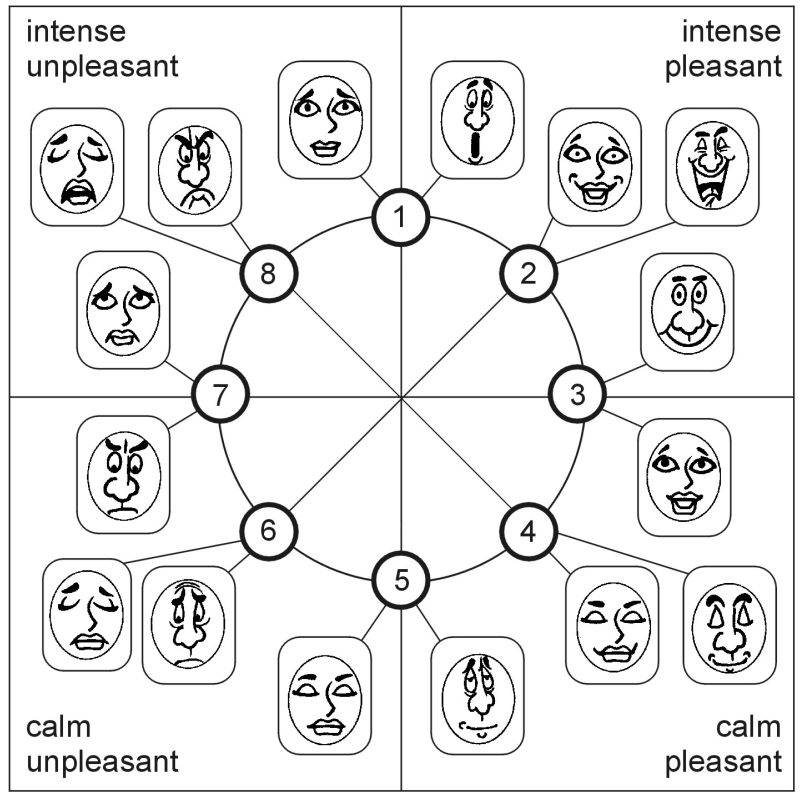
\includegraphics[width=0.5\textwidth]{img/Emocards.png}
        \fonte{Author.}
\end{figure}

\subsubsection{Results Analysis}

Esta seção apresenta os resultados obtidos da execução do \ac{ex2}.
Todos os testes estatísticos foram feitos utilizando a linguagem R com a IDE RStudio. 
Os scripts para este experimento estão disponíveis de forma pública em um repositório\footnote{\url{ https://github.com/JonnathanRiquelmo/misc/blob/main/some-scripts.r }}, portanto desta forma qualquer pessoa pode, além de consultar todos os dados brutos, executá-los localmente e verificar os resultados.

Levamos em consideração as mesmas hipóteses anteriores, relacionadas ao esforço (tempo) necessário e efetividade (qualidade) alcançada pelos modelos feitos.
Para a avaliação referente ao esforço foram utilizados o teste de normalidade Shapiro-Wilk, em razão da amostra ter menos de trinta (30) elementos, e o Teste T pareado para amostras dependentes, em que foi levado em consideração os tempos coletados durante a execução das atividades de modelagem do experimento. 

O método Shapiro-Wilk testa a hipótese nula de que uma distribuição é normal, mediante o cálculo do valor $W$, onde após é então verificado na tabela do teste\footnote{\url{ http://www.uel.br/projetos/experimental/pages/arquivos/Probabilidades\_Shapiro.pdf }} se ocorre a rejeição ou aceitação da hipótese. 
O cálculo do método Shapiro-Wilk é dado conforme a fórmula da Equação \ref{eq:Shapiro}: 

\begin{equation}
\label{eq:Shapiro}
%\[ 
W = \frac{\left(\sum_{i=1}^{n} a_ix_{(i)}\right)^2}{\sum_{i=1}^{n}\left(x_i -\overline{x}\right)} 
%\]
\end{equation}

Uma forma simplificada do Teste T pareado para amostras dependentes
se dá conforme a fórmula da Equação \ref{eq:TestT}:

\begin{equation}
\label{eq:TestT}
%\[ 
t = \frac{m}{s/\sqrt{n}} 
%\]
\end{equation}

Nesta fórmula o \textit{\textbf{m}} e o \textit{\textbf{s}} são a média e o desvio padrão da diferença (\textbf{\textit{d}}), respectivamente. 
O \textit{\textbf{n}} corresponde ao tamanho de \textbf{\textbf{d}}, ou seja, o tamanho da amostra.
Este teste de hipótese é usado para comparar as médias de duas amostras relacionadas, ou seja, quando se possui dois valores (par de valores) para uma mesma amostra. 
Contudo, para comparar as médias dos dois conjuntos de dados emparelhados, as diferenças entre todos os pares devem ser calculadas primeiro.
O nível de significância alfa ($\alpha$) utilizado foi de cinco por cento (5\%).

Para os testes da efetividade foram adotados os mesmos métodos estatísticos, porém ao invés do uso da métrica de tempo gasto nas atividades, foi necessário outra grandeza.
Sendo assim, foram realizados novamente cálculos para uma medida F1, conforme descrito anteriormente na Seção \ref{ssec_experiments:preliminary_planning}.


A partir dos valores brutos dos tempos foi calculada a diferença para ser possível realizar o teste de normalidade Shapiro-Wilk.
Por ser um teste estatístico, esta técnica tem como produto a medida do valor-$p$.
Para este teste foi adotado um nível de significância $\alpha$~=~5\%. 
Isso significa que se o valor-$p$ for menor que 5\% ($p$ < 0.05), a hipótese nula de que a distribuição é normal deve ser rejeitada.

Após os cálculos com o conjunto das diferenças dos tempos chegou-se a um valor-$p$ de 0.5991.
Como valor-$p$ \textgreater $\alpha$, a hipótese nula foi aceita, concluindo assim que os dados são normalmente distribuídos.
Em outras palavras, a diferença entre a amostra de dados e a distribuição normal não é grande o suficiente para ser estatisticamente significativa.

É importante ressaltar que quanto maior o valor-$p$, mais ele suporta uma hipótese nula. 
No caso do resultado obtido a chance de erro do tipo 1 (rejeitar uma hipótese nula que é correta) é muito alta, podendo ser traduzida em 59,91\% (0.5991).
Ainda em relação ao teste de normalidade, o valor de \textit{W} calculado foi de 0.968, estando dentro do intervalo aceito do valor crítico de 95\%. 
Isto significa que existe 95\% de chances da amostra ter origem em uma população normal.

Tendo sido a amostra testada quanto à sua normalidade, foi possível realizar o teste da primeira hipótese estabelecida neste experimento. 
No teste T pareado para amostras dependentes foi utilizado um nível de significância $\alpha$~=~5\%, com o qual se chegou a uma medida de 0.3492 para o valor-$p$. 

Por ser um teste bicaudal, ou seja, que inclui uma igualdade na sua hipótese nula, esse valor-$p$ não mostra evidências suficientes para garantir a rejeição da afirmativa de $H_0 : \mu Tempo_G = \mu Tempo_T$.
Em resumo, a média dos valores da abordagem gráfica (brModelo) é considerada similar à média da população da abordagem textual (ERtext).
Em outras palavras, a diferença entre as médias d brModelo e da ERtext não é grande o suficiente para ser estatisticamente significativa.
A Figura \ref{fig:boxplotTempo2} exibe um gráfico boxplot com a variação observada dos dados obtidos. 
% A \ref{tab:ResultsModelosGeral2} mostra os valores que possibilitam uma análise de dispersão. 


% \textbf{NORMALIDADE DAS AMOSTRAS}\\
% Método: \textbf{Shapiro-Wilk} (amostra com menos de 30 elementos)\\~\\

% \textbf{TEMPO}\\
% \textbf{P-value	= 0.5991} com com $\alpha$~=~5\%  (Significance level)\\
% Sample size (n)	25\\
% Os testes de Shapiro-Wilk não mostraram um desvio significativo da normalidade, W(25) = 0,968, p = 0,5991\\
% Ou seja, o conjunto da diferença entre os valores dos tempos de execução de cada tratamento (textual X gráfico) pode ser cosiderado uma \textbf{distribuição normal}.
% \\~\\ 
% \textbf{MEDIDA-F}\\
% \textbf{P-value = 0.5166} com $\alpha$~=~5\% (Significance level)\\
% Sample size (n)	25\\
% Os testes de Shapiro-Wilk não mostraram um desvio significativo da normalidade, W(25) = 0,965, p = 0,5166\\
% Ou seja, o conjunto da diferença entre os valores das medidas-F de cada tratamento (textual X gráfico) pode ser cosiderado uma \textbf{distribuição normal}.


% \\~\\

% \textbf{TESTE DE HIPÓTESE}\\
% Método: \textbf{Teste T pareado (amostras dependentes, com menos de 30 elementos)}\\~\\
% \textbf{MEDIDA-F}\\
% P-value	= 0.2147 com $\alpha$~=~5\% (Significance level)\\ 
% Sample size (n)	25\\
% Como o valor de P \textgreater $\alpha$, \textbf{H0 não pode ser rejeitada}.
% A média dos valores da brModelo é considerada igual à média da população da ERtext.
% Em outras palavras, a \textbf{diferença} entre as médias d brModelo e da ERtext \textbf{não é grande o suficiente para ser estatisticamente significativa}.\\
% \textbf{Lembrete: Um resultado de não significância não pode provar que H0 está correta, apenas que a suposição nula não pode ser rejeitada, ou seja, não se aceita H0 mas sim deixa-se de rejeitar H0.}
% \\~\\ 
% \textbf{TEMPO}\\
% P-value = 0.3492 com $\alpha$~=~5\% (Significance level)\\
% Sample size (n)	25\\
% Como o valor de P \textgreater $\alpha$, \textbf{H0 não pode ser rejeitada}.
% A média dos valores da brModelo é considerada igual à média da população da ERtext.
% Em outras palavras, a \textbf{diferença} entre as médias d brModelo e da ERtext \textbf{não é grande o suficiente para ser estatisticamente significativa}.

\begin{figure}[!htb]
        \centering
        \caption{Esforço (tempo) dos tratamentos no segundo experimento.}
        \label{fig:boxplotTempo2}
        \begin{filecontents*}{data2.csv}
24,24,28,28,29,30,30,30,31,33,35,38,38,44,45,46,46,46,53,58,61,70,74,90,102
21,23,25,29,30,30,31,32,35,36,40,40,43,44,47,50,50,55,55,55,67,74,93,93,171
\end{filecontents*}

\makeatletter
\pgfplotsset{
    boxplot/hide outliers/.code={
        \def\pgfplotsplothandlerboxplot@outlier{}%
    }
}
\makeatother

\begin{tikzpicture}
    \pgfplotstableread[col sep=comma]{data2.csv}\csvdata
    % Boxplot groups columns, but we want rows
    \pgfplotstabletranspose\datatransposed{\csvdata} 
    \begin{axis}[
        boxplot/draw direction=y,
        xtick={1, 2},
        ylabel={\scriptsize Time (minutes)},
        xticklabels={{\scriptsize Graphical Treatment}, {\scriptsize Textual Treatment}},
        height=7cm,
        width=10cm,
        % boxplot/draw direction = y,
        % axis x line* = bottom,
        % axis y line = left,
        % enlarge y limits,
        ymajorgrids,
        % xtick = {1, 2},
        % xticklabel style = {align=center, font=\small},
        % xticklabels = {Graphical Treatment, Textual Treatment},
        % ylabel = {Time (minutes)},
        ytick = {15, 30, 45, 60, 75, 90,  105, 120, 135, 150, 165, 180},
        yticklabel style = {font=\scriptsize}
    ]
        \foreach \n in {1,...,2} {
            \addplot+[boxplot, /pgfplots/boxplot/hide outliers, fill, fill opacity=0.4, draw=black] table[y index=\n] {\datatransposed};
        }
    \end{axis}
\end{tikzpicture}


        \fonte{Author.}
\end{figure}



Para avaliar a hipotése referente a efetividade do uso das abordagens, os artefatos produzidos pelos sujeitos foram avaliados conforme os modelos de referência previamente estabelecidos.

Como dito, nesta avaliação foi utilizada a medida F1, uma medida proveniente da área de reconhecimento de padrões e recuperação de informação. 
Essa medida representa a combinação da precisão e revocabilidade observada de um resultado em relação à uma referência.

Após a obtenção dos valores F1 de cada modelo, foi realizado o teste de normalidade Shapiro-Wilk.
Após os cálculos com o conjunto das diferenças da medida F1 de cada modelo, chegou-se a um valor-$p$ de 0.5166.
Com este resultado obtido a chance de erro do tipo 1 (rejeitar uma hipótese nula que é correta) pode ser muito alta, podendo ser traduzida em 51,66\% (0.5166).

Como o valor-$p$ \textgreater $\alpha$, a hipótese nula foi aceita, constatando assim que os dados são normalmente distribuídos, isto é, a diferença entre a amostra de dados e uma distribuição normal não é grande o suficiente para ser estatisticamente significativa.

Após a amostra ser testada quanto à sua normalidade, foi realizado o teste da segunda hipótese definida, relativa a efetividade (qualidade) das abordagens. 
Desta vez, no teste T pareado para amostra dependentes, novamente foi utilizado um nível de significância $\alpha$~=~5\%, com o qual se chegou a uma medida de 0.2147 para o valor-$p$. 

Pela afirmativa original incluir uma igualdade, caracterizando também este teste como bicaudal, chegou-se a conclusão que o valor-$p$ calculado demonstra que não há evidências suficientes para garantir a rejeição da afirmativa da hipótese nula original, denotada como $H_0 : \mu Efetividade_G = \mu Efetividade_T$.
Logo, a hipótese nula de que as abordagens possuem efetividades iguais é aceita, pois segundo o teste a diferença média da medida F1 entre os tratamentos não é estatisticamente significativa.
A Figura \ref{tab:ResultsModelosGeral2} apresenta as medidas médias dos valores avaliados, e também fornecem a possibilidade para a realização de uma análise de dispersão.

\rowcolors{1}{gray!15}{white}
\begin{table}[!htb]
    \caption{Measures of the conceptual data models produced in the second experiment.}
    \label{tab:ResultsModelosGeral2}
    \centering
    % \scriptsize
    \tiny
    \begin{tabular}{l|ccccc|ccccc}%{l|ccccc|ccccc}
    \bottomrule
    \rowcolor[HTML]{C0C0C0}
    \multicolumn{1}{l}{} &
    \multicolumn{5}{c|}{\textbf{Graphical Treatment}} &
    \multicolumn{5}{c}{\textbf{Textual Treatment}}
    \\ 
    \hline
    \rowcolor[HTML]{C0C0C0}
    \textbf{Measure} & \textbf{MI} & \textbf{RI} & \textbf{P(\%)} & \textbf{R(\%)} & \textbf{F1(\%)} &
    \textbf{MI} & \textbf{RI} & \textbf{P(\%)} & \textbf{R(\%)} & \textbf{F1(\%)}
    \\
    \hline
Maximum	&	49.00	&	44.00	&	93.75	&	92.50	&	91.67	&	65.00	&	45.00	&	94.74	&	92.68	&	91.14	\\
3\textdegree Quartile	&	46.00	&	39.00	&	88.89	&	85.42	&	86.02	&	47.00	&	38.00	&	89.19	&	87.80	&	87.06	\\
Average	&	41.08	&	35.20	&	85.88	&	78.57	&	81.74	&	44.64	&	36.48	&	83.24	&	83.35	&	82.81	\\
Median	&	43.00	&	36.00	&	86.05	&	77.50	&	81.32	&	44.00	&	36.00	&	85.37	&	83.67	&	84.71	\\
1\textdegree Quartile	&	36.00	&	31.00	&	84.78	&	75.00	&	79.12	&	40.00	&	34.00	&	81.82	&	79.59	&	78.72	\\
Minimum	&	27.00	&	23.00	&	71.43	&	57.50	&	68.66	&	34.00	&	32.00	&	58.46	&	69.39	&	69.47	\\
Variance	&	34.63	&	23.84	&	20.21	&	72.57	&	26.91	&	59.59	&	10.25	&	102.43	&	34.72	&	37.18	\\
SD	&	5.89	&	4.88	&	4.50	&	8.52	&	5.19	&	7.72	&	3.20	&	10.12	&	5.89	&	6.10	\\
    \toprule
\end{tabular}
\begin{tablenotes}
    \scriptsize
    \centering
    \item \textit{Legend: MI = Modeled Items; RI = Relevant Items; P = Precision; R = Recall; F1 = F1-Score; SD = Standard Deviation.}
\end{tablenotes}
\fonte{Author.}
\end{table}

O gráfico boxplot da Figura \ref{fig:boxplotMedidaF2} exibe uma representação visual da medida F1 dos tratamentos aplicados.
Com base neste gráfico é possível verificar o resultado obtido no teste de hipótese pois a dispersão dos dados não apresenta grande diferença entre as abordagens. 

\begin{figure}[!htb]
        \centering
        \caption{Medida-F (qualidade) dos tratamentos no segundo experimento.}
        \label{fig:boxplotMedidaF2}
        \include{img/boxplotMedidaF2}
        \fonte{Author.}
\end{figure}

A avaliação referente aos atributos de qualidade para as ferramentas é apresentado na Figura \ref{fig:inst3GERALExp2}.
No geral os participantes a avaliação dos participantes foi proporcionalmente similar a obtida no experimento anterior. 
% Os destaques desta vez ficaram por conta do atributo de satisfação para a abordagem textual, enquanto os atributos de conformidade e compreensão se sairam melhores na abordagem gráfica. 
% Outro ponto a ser ressaltado é a diferença levemente menor no atributo de produtividade, mas ainda em favor da abordagem textual.

\begin{figure}[!htb]
    \centering
    \caption{Avaliação dos atributos de qualidadade no segundo experimento.}
    \label{fig:inst3GERALExp2}
    \pgfplotsset{testbar/.style={
        xbar stacked,
        legend cell align=left,
        legend style={
            legend columns=8,
            font=\scriptsize,
            at={(xticklabel cs:1.0)},
            anchor=north east,
            draw=none,
            nodes={scale=1}
            },
        width=10cm,
        axis y line*= none, 
        axis x line*= bottom,
        xmajorgrids = false,
        xmin=0,xmax=25,
        ytick = data,
        yticklabels = {
            {\scriptsize Conformity-ERtext},
            {\scriptsize Conformity-brModelo},
            {\scriptsize Understandability-ERtext}, %Intelligibility
            {\scriptsize Understandability-brModelo},
            {\scriptsize Learnability-ERtext}, %Apprehensibility
            {\scriptsize Learnability-brModelo}, 
            {\scriptsize Operability-ERtext},
            {\scriptsize Operability-brModelo},
            {\scriptsize Quality in Use-ERtext},
            {\scriptsize Quality in Use-brModelo},
            {\scriptsize Productivity-ERtext}, %Performance Efficiency
            {\scriptsize Productivity-brModelo},
            {\scriptsize Satisfaction-ERtext},
            {\scriptsize Satisfaction-brModelo}
        },
        tick align = outside, 
        xtick pos = left,
        xticklabel style = {font=\scriptsize},
        bar width=5mm, 
        y=7mm,
        enlarge y limits={abs=0.450},% 0.5 + 0.5*(y - bar width)/y [TeX.sx #47995]
        nodes near coords,
        nodes near coords align=center,%Move values in bar
        every node near coord/.append style={
            black,
            font=\scriptsize,
            text opacity=1,
            fill=white,
            fill opacity=0.5,
            outer sep=\pgflinewidth
        }
    }}
    \begin{tikzpicture}
    \begin{axis}[testbar] 
    \addplot[pattern color=red,pattern=north east lines] coordinates
        {(0,14)(0,13)(0,12)(0,11)(0,10)(0,9)(0,8)(1,7)(0,6)(0,5)(0,4)(1,3)(0,2)(1,1)};
    \addplot[pattern color=teal,pattern=vertical lines] coordinates
        {(0,14)(0,13)(0,12)(0,11)(2,10)(1,9)(1,8)(2,7)(0,6)(1,5)(1,4)(2,3)(0,2)(1,1)};
    \addplot[pattern color=gray, pattern=grid] coordinates
       {(0,14)(1,13)(1,12)(0,11)(3,10)(3,9)(2,8)(4,7)(2,6)(1,5)(2,4)(2,3)(2,2)(4,1)};
    \addplot[pattern color=magenta, pattern=north west lines] coordinates
       {(6,14)(4,13)(5,12)(5,11)(8,10)(6,9)(6,8)(7,7)(5,6)(2,5)(5,4)(5,3)(4,2)(3,1)};
    \addplot[pattern color=blue, pattern=horizontal lines] coordinates
       {(10,14)(5,13)(8,12)(7,11)(7,10)(9,9)(10,8)(6,7)(11,6)(9,5)(9,4)(9,3)(4,2)(7,1)};
    \addplot[pattern color=green, pattern=crosshatch dots] coordinates
       {(9,14)(15,13)(11,12)(13,11)(5,10)(6,9)(6,8)(5,7)(7,6)(12,5)(8,4)(6,3)(15,2)(9,1)};
    \legend{1-Disagree, 2, 3, 4, 5, 6-Agree}
    \end{axis}
    \end{tikzpicture}
    
% \begin{tikzpicture}
% \begin{axis}[
%     xbar stacked,
%     legend cell align=center,
%     legend style={
%     legend columns=5,
%         at={(xticklabel cs:1.0)},
%         anchor=north east,
%         draw=none
%     },
%     ytick=data,
%     axis y line*=none,
%     axis x line*=bottom,
%     tick label style={font=\small},
%     legend style={font=\small},
%     label style={font=\small},
%     xtick={0,3,6},
%     xticklabel= {},
%     bar width=5mm,
%     ylabel={Questions},
%     yticklabels={P-Q1, T-Q1, P-Q2, T-Q2, P-Q3, T-Q3, P-Q4, T-Q4,P-Q5, T-Q5,P-Q6, T-Q6, P-Q7, T-Q7},
%     xmin=0,
%     xmax=6,
%     area legend,
%     y=6.5mm,
%     enlarge y limits={abs=0.625},
%     nodes near coords,
%     nodes near coords align=center,
%     every node near coord/.append style={
%         black,
%         font=\small,
%         text opacity=.65,
%         fill=white,
%         fill opacity=0.75,
%         outer sep=\pgflinewidth
%     }
% ]
% \addplot[pattern color=red,pattern=horizontal lines] coordinates
% {(0,14)(0,13)(0,12)(0,11) (3,10)(0,9)(0,8) (0,7) (0,6)(0,5)(0,4) (0,3) (0,2) (0,1)};   
% \addplot[pattern color=orange,pattern=grid] coordinates
% {(3,14) (0,13)(0,12)(0,11)(2,10) (1,9)(1,8)(0,7)(3,6)(0,5)(0,4)(3,3) (4,2) (0,1) };  
% \addplot[pattern color = green, pattern=crosshatch dots] coordinates
% {(0,14) (0,13) (3,12)(2,11)(1,10) (3,9)(4,8)(1,7)(3,6)(1,5)(3,4)(2,3)(2,2) (2,1) };   
% \addplot[pattern color=blue, pattern =vertical lines ] coordinates
% {(2,14) (3,13) (2,12)(3,11)(0,10)(2,9)(1,8)(4,7)(0,6)(3,5) (3,4)(1,3)(0,2)(4,1)};   
% \addplot[pattern color=gray, pattern = dots] coordinates
% {(1,14)(3,13)(1,12)(1,11)(0,10)(0,9)(0,8)(1,7) (0,6)(2,5) (0,4)(0,3)(0,2)(0,1) };   
% \legend{1-Disagree, 2, 3, 4, 5-Agree}

% \end{axis}
% \end{tikzpicture}
% \footnotesize
% T-Thoth answers; P-Parsifal answers;






% \begin{tikzpicture}
% \begin{axis}[
%     xbar stacked,
%     legend cell align=left,
%     legend style={
%     legend columns=2,
%         at={(xticklabel cs:1.0)},
%         anchor=north east,
%         draw=none
%     },
%     ytick=data,
%     axis y line*=none,
%     axis x line*=bottom,
%     tick label style={font=\scriptsize},
%     legend style={font=\scriptsize},
%     %legend style={font=\scriptsize,row sep=-0.1cm,/tikz/every odd column/.append style={column sep=0.01cm}},
%     label style={font=\scriptsize},
%     xtick={0,10,...,100},
%     width=\columnwidth,
%     bar width=3.5mm,
%     % xlabel={Frequencia em \%},
%     yticklabels={
%     {Q1 - OC},
%     {Q2 - TD},
%     {Q3 - OC},
%     {Q4 - TD},
%     {Q5 - OC},
%     {Q6 - TD},
%     {Q7 - OC},
%     {Q8 - TD},
%     {Q9 - OC},
%     {Q10 - TD},
%     {Q11 - OC},
%     {Q12 - TD}},
%     xmin=0,
%     xmax=100,
%     area legend,
%     y=5mm,
%     enlarge y limits={abs=0.625},
%     nodes near coords,
%     nodes near coords={\pgfmathprintnumber\pgfplotspointmeta\%},
%     nodes near coords align=center,%Move values in bar
%     every node near coord/.append style={
%         black,
%         font=\footnotesize,
%         text opacity=1,
%         fill=white,
%         fill opacity=0.7,
%         outer sep=\pgflinewidth
%     }
% ]
% \addplot[pattern color=blue,pattern=dots] coordinates
% {(0,0)(0,1)(0,2)(0,3)(0,4)(0,5)(0,6)(0,7)(0,8)(0,9)(0,10)(0,11)};
% \addplot[pattern color=red, pattern=vertical lines] coordinates
% {(4,0)(32,1)(0,2)(9,3)(13,4)(18,5)(0,6)(9,7)(5,8)(5,9)(0,10)(14,11)};
% \addplot[pattern color=cyan, pattern=grid] coordinates
% {(27,0)(9,1)(4,2)(5,3)(23,4)(27,5)(36,6)(23,7)(27,8)(41,9)(46,10)(45,11)};
% \addplot[pattern color=green, pattern=horizontal lines] coordinates
% {(55,0)(32,1)(55,2)(68,3)(41,4)(50,5)(46,6)(64,7)(64,8)(45,9)(36,10)(27,11)};
% \addplot[pattern color=orange, pattern=crosshatch dots] coordinates
% {(14,0)(27,1)(41,2)(18,3)(23,4)(5,5)(18,6)(4,7)(4,8)(9,9)(18,10)(14,11)};
% \legend{Strongly disagree,Disagree,Neither agree nor disagree,Agree,Strongly agree}; 

% \end{axis}  
% \end{tikzpicture}d
    \fonte{Author.}
\end{figure}

A avaliação referente aos construtores da DSL da abordagem textual, os resultados também seguiram a mesma proporção observada no primeiro experimento.
Isso nos leva a concluir que de fato é necessário uma reavaliação da representação dos relacionamentos ternários para torná-los mais fáceis de aprender, interpretar e utilizar.

\begin{figure}[!htb]
    \centering
    \caption{Avaliação dos contrutores da DSL no segundo experimento.}
    \label{fig:inst4GERALExp2}
    \pgfplotsset{testbar/.style={
            xbar stacked,
            legend cell align=left,
            legend style={
                legend columns=6,
                font=\scriptsize,
                at={(xticklabel cs:1.0)},
                anchor=north east,
                draw=none
                },
            width=10cm,
            axis y line*= none, 
            axis x line*= bottom,
            xmajorgrids = false,
            xmin=0,xmax=25,
            ytick = data,
            yticklabels = {
            {\scriptsize Entity}, 
            {\scriptsize Referential Attribute},
            {\scriptsize Descriptive Attribute},
            {\scriptsize Binary Relationship},
            {\scriptsize Ternary Relationship}, 
            {\scriptsize Self-relationship},
            {\scriptsize Cardinality},
            {\scriptsize Generalization}
            },
            tick align = outside, 
            xticklabel style = {font=\scriptsize},
            xtick pos = left,
             bar width=3.5mm, 
             y=6.5mm,
             enlarge y limits={abs=0.450},% 0.5 + 0.5*(y - bar width)/y [TeX.sx #47995] #47995]
            nodes near coords,
            nodes near coords align=center,%Move values in bar
            every node near coord/.append style={
                black,
                font=\scriptsize,
                text opacity=1,
                fill=white,
                fill opacity=0.5,
                outer sep=\pgflinewidth
            }
        }}
    \begin{tikzpicture}
    \begin{axis}[testbar] 
    \addplot[pattern color=red,pattern=north east lines] coordinates
        {(0,8)(0,7)(0,6)(0,5)(0,4)(0,3)(0,2)(0,1)};
    \addplot[pattern color=teal,pattern=vertical lines] coordinates
        {(0,8)(0,7)(0,6)(1,5)(2,4)(1,3)(0,2)(0,1)};   
    \addplot[pattern color=gray, pattern=grid] coordinates
        {(0,8)(0,7)(2,6)(2,5)(5,4)(0,3)(0,2)(3,1)};   
    \addplot[pattern color=magenta, pattern=north west lines] coordinates
        {(3,8)(4,7)(2,6)(0,5)(6,4)(3,3)(0,2)(3,1)};   
    \addplot[pattern color=blue, pattern=horizontal lines] coordinates
        {(4,8)(4,7)(6,6)(11,5)(7,4)(5,3)(5,2)(6,1)}; 
    \addplot[pattern color=green, pattern=crosshatch dots] coordinates
        {(18,8)(17,7)(15,6)(11,5)(5,4)(16,3)(20,2)(13,1)};
    \legend{1-Disagree, 2, 3, 4, 5, 6-Agree}
    \end{axis}
    \end{tikzpicture}

% \begin{figure}[!ht]
% \centering
% \caption{Resultados do formulários de avaliação.}
% \begin{tikzpicture}
% \begin{axis}[
%     xbar stacked,
%     legend cell align=center,
%     legend style={
%     legend columns=5,
%         at={(xticklabel cs:1.0)},
%         anchor=north east,
%         draw=none
%     },
%     ytick=data,
%     axis y line*=none,
%     axis x line*=bottom,
%     tick label style={font=\small},
%     legend style={font=\small},
%     label style={font=\small},
%     xtick={0,5,10},
%     xticklabel= {},
%     bar width=7mm,
%     ylabel={Formulário/Grupo},
%     yticklabels={F1-C, F1-E, F2-C, F2-E, F3-C, F3-E},
%     xmin=0,
%     xmax=10,
%     area legend,
%     y=9mm,
%     enlarge y limits={abs=0.825},
%     nodes near coords,
%     nodes near coords align=center,
%     every node near coord/.append style={
%         black,
%         font=\small,
%         text opacity=.65,
%         fill=white,
%         fill opacity=0.6,
%         outer sep=\pgflinewidth
%     }
% ]
% %NOTA 1
% \addplot[pattern color=red,pattern=horizontal lines] coordinates
% {(0,6)(0,5)(0,4)(0,3)(0,2)(0,1)};
% %NOTA 2
% \addplot[pattern color=orange,pattern=grid] coordinates
% {(1,6)(1,5)(1,4)(0,3)(1,2)(0,1)};   
% \addplot[pattern color = green, pattern=crosshatch dots] coordinates
% % NOTA 3
% {(3,6)(3,5)(5,4)(2,3)(5,2)(1,1)};   
% \addplot[pattern color=blue, pattern =vertical lines ] coordinates
% %NOTA 4
% {(2,6)(3,5)(1,4)(4,3)(3,2)(3,1)};   
% \addplot[pattern color=gray, pattern = dots] coordinates
% %NOTA 5
% {(3,6)(3,5)(2,4)(4,3)(0,2)(6,1)};   
% \legend{1-Disagree, 2, 3, 4, 5-Agree}

% \end{axis}
% \end{tikzpicture}
% \footnotesize
% \label{img:respostas1}
% 	\fonte{O autor.}
% \end{figure}
    \fonte{Author.}
\end{figure}

\clearpage

A avaliação dos EMOCARDS...

\begin{figure}[!htb]
    \centering
    \caption{Emocards segundo experimento - ERtext}
    \label{fig:Emocards1_alt}
    

\tikzset{every picture/.style={line width=0.75pt}} %set default line width to 0.75pt        

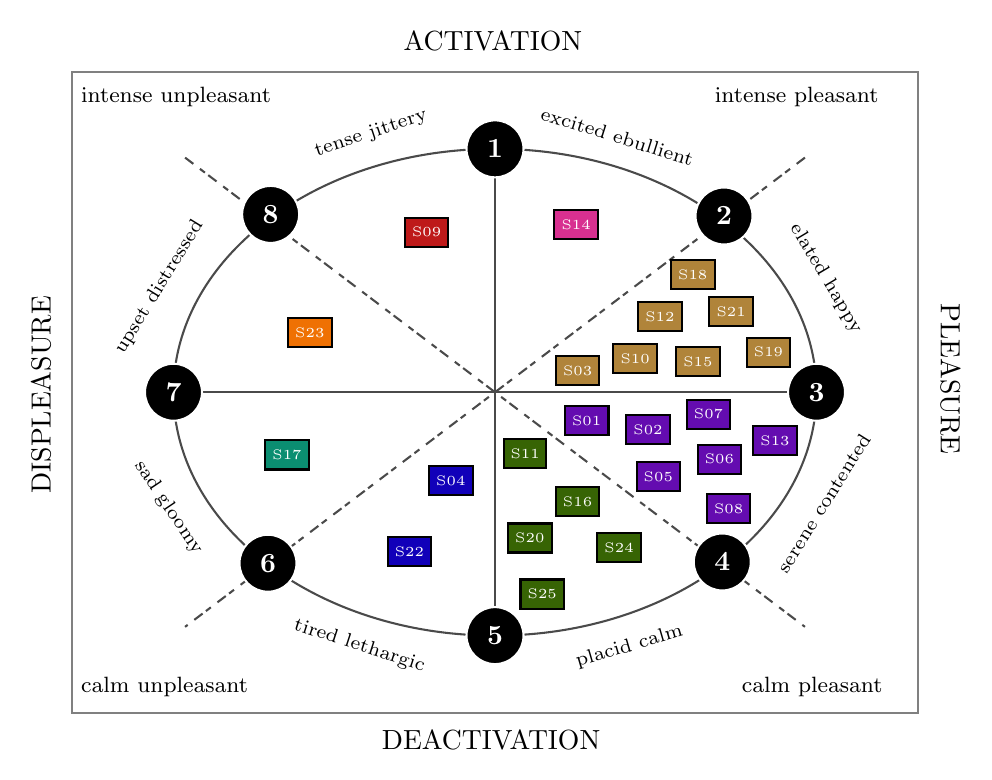
\begin{tikzpicture}[x=0.75pt,y=0.75pt,yscale=-1,xscale=1]
%uncomment if require: \path (0,389); %set diagram left start at 0, and has height of 389

%Flowchart: Or [id:dp3592995680476845] 
\draw  [color={rgb, 255:red, 74; green, 74; blue, 74 }  ,draw opacity=1 ] (182.64,181.1) .. controls (182.64,116.34) and (252,63.84) .. (337.55,63.84) .. controls (423.11,63.84) and (492.46,116.34) .. (492.46,181.1) .. controls (492.46,245.86) and (423.11,298.36) .. (337.55,298.36) .. controls (252,298.36) and (182.64,245.86) .. (182.64,181.1) -- cycle ; \draw  [color={rgb, 255:red, 74; green, 74; blue, 74 }  ,draw opacity=1 ] (182.64,181.1) -- (492.46,181.1) ; \draw  [color={rgb, 255:red, 74; green, 74; blue, 74 }  ,draw opacity=1 ] (337.55,63.84) -- (337.55,298.36) ;
%Straight Lines [id:da30798451784186187] 
\draw [color={rgb, 255:red, 74; green, 74; blue, 74 }  ,draw opacity=1 ] [dash pattern={on 3.75pt off 3pt on 2.25pt off 1.5pt}]  (188.22,68.06) -- (486.88,294.14) ;
%Straight Lines [id:da7804870395610348] 
\draw [color={rgb, 255:red, 74; green, 74; blue, 74 }  ,draw opacity=1 ] [dash pattern={on 3.75pt off 3pt on 2.25pt off 1.5pt}]  (486.88,68.06) -- (188.22,294.14) ;
%Shape: Rectangle [id:dp23344423808181314] 
\draw  [color={rgb, 255:red, 128; green, 128; blue, 128 }  ,draw opacity=1 ] (133.68,26.77) -- (541.42,26.77) -- (541.42,335.43) -- (133.68,335.43) -- cycle ;

% Text Node
\draw  [color={rgb, 255:red, 0; green, 0; blue, 0 }  ,draw opacity=1 ][fill={rgb, 255:red, 100; green, 12; blue, 176 }  ,fill opacity=1 ]  (400.79,192.22) -- (421.79,192.22) -- (421.79,206.22) -- (400.79,206.22) -- cycle  ;
\draw (411.29,199.22) node  [font=\tiny,color={rgb, 255:red, 255; green, 255; blue, 255 }  ,opacity=1 ] [align=left] {S02};
% Text Node
\draw  [color={rgb, 255:red, 0; green, 0; blue, 0 }  ,draw opacity=1 ][fill={rgb, 255:red, 55; green, 100; blue, 4 }  ,fill opacity=1 ]  (342.09,203.64) -- (362.09,203.64) -- (362.09,217.64) -- (342.09,217.64) -- cycle  ;
\draw (352.09,210.64) node  [font=\tiny,color={rgb, 255:red, 255; green, 255; blue, 255 }  ,opacity=1 ] [align=left] {S11};
% Text Node
\draw  [color={rgb, 255:red, 0; green, 0; blue, 0 }  ,draw opacity=1 ][fill={rgb, 255:red, 176; green, 132; blue, 58 }  ,fill opacity=1 ]  (366.87,163.61) -- (387.87,163.61) -- (387.87,177.61) -- (366.87,177.61) -- cycle  ;
\draw (377.37,170.61) node  [font=\tiny,color={rgb, 255:red, 255; green, 255; blue, 255 }  ,opacity=1 ] [align=left] {S03};
% Text Node
\draw  [color={rgb, 255:red, 0; green, 0; blue, 0 }  ,draw opacity=1 ][fill={rgb, 255:red, 100; green, 12; blue, 176 }  ,fill opacity=1 ]  (461.95,197.33) -- (482.95,197.33) -- (482.95,211.33) -- (461.95,211.33) -- cycle  ;
\draw (472.45,204.33) node  [font=\tiny,color={rgb, 255:red, 255; green, 255; blue, 255 }  ,opacity=1 ] [align=left] {S13};
% Text Node
\draw  [color={rgb, 255:red, 0; green, 0; blue, 0 }  ,draw opacity=1 ][fill={rgb, 255:red, 183; green, 0; blue, 0 }  ,fill opacity=0.9 ]  (294.12,96.99) -- (315.12,96.99) -- (315.12,110.99) -- (294.12,110.99) -- cycle  ;
\draw (304.62,103.99) node  [font=\tiny,color={rgb, 255:red, 255; green, 255; blue, 255 }  ,opacity=1 ] [align=left] {S09};
% Text Node
\draw  [color={rgb, 255:red, 0; green, 0; blue, 0 }  ,draw opacity=1 ][fill={rgb, 255:red, 100; green, 12; blue, 176 }  ,fill opacity=1 ]  (371.22,187.92) -- (392.22,187.92) -- (392.22,201.92) -- (371.22,201.92) -- cycle  ;
\draw (381.72,194.92) node  [font=\tiny,color={rgb, 255:red, 255; green, 255; blue, 255 }  ,opacity=1 ] [align=left] {S01};
% Text Node
\draw  [color={rgb, 255:red, 0; green, 0; blue, 0 }  ,draw opacity=1 ][fill={rgb, 255:red, 100; green, 12; blue, 176 }  ,fill opacity=1 ]  (405.75,214.64) -- (426.75,214.64) -- (426.75,228.64) -- (405.75,228.64) -- cycle  ;
\draw (416.25,221.64) node  [font=\tiny,color={rgb, 255:red, 255; green, 255; blue, 255 }  ,opacity=1 ] [align=left] {S05};
% Text Node
\draw  [color={rgb, 255:red, 0; green, 0; blue, 0 }  ,draw opacity=1 ][fill={rgb, 255:red, 17; green, 0; blue, 185 }  ,fill opacity=1 ]  (305.76,216.61) -- (326.76,216.61) -- (326.76,230.61) -- (305.76,230.61) -- cycle  ;
\draw (316.26,223.61) node  [font=\tiny,color={rgb, 255:red, 255; green, 255; blue, 255 }  ,opacity=1 ] [align=left] {S04};
% Text Node
\draw  [color={rgb, 255:red, 0; green, 0; blue, 0 }  ,draw opacity=1 ][fill={rgb, 255:red, 176; green, 132; blue, 58 }  ,fill opacity=1 ]  (424.83,159.33) -- (445.83,159.33) -- (445.83,173.33) -- (424.83,173.33) -- cycle  ;
\draw (435.33,166.33) node  [font=\tiny,color={rgb, 255:red, 255; green, 255; blue, 255 }  ,opacity=1 ] [align=left] {S15};
% Text Node
\draw  [color={rgb, 255:red, 0; green, 0; blue, 0 }  ,draw opacity=1 ][fill={rgb, 255:red, 100; green, 12; blue, 176 }  ,fill opacity=1 ]  (435.18,206.39) -- (456.18,206.39) -- (456.18,220.39) -- (435.18,220.39) -- cycle  ;
\draw (445.68,213.39) node  [font=\tiny,color={rgb, 255:red, 255; green, 255; blue, 255 }  ,opacity=1 ] [align=left] {S06};
% Text Node
\draw  [color={rgb, 255:red, 0; green, 0; blue, 0 }  ,draw opacity=1 ][fill={rgb, 255:red, 100; green, 12; blue, 176 }  ,fill opacity=1 ]  (439.6,230.11) -- (460.6,230.11) -- (460.6,244.11) -- (439.6,244.11) -- cycle  ;
\draw (450.1,237.11) node  [font=\tiny,color={rgb, 255:red, 255; green, 255; blue, 255 }  ,opacity=1 ] [align=left] {S08};
% Text Node
\draw  [color={rgb, 255:red, 0; green, 0; blue, 0 }  ,draw opacity=1 ][fill={rgb, 255:red, 176; green, 132; blue, 58 }  ,fill opacity=1 ]  (394.61,157.99) -- (415.61,157.99) -- (415.61,171.99) -- (394.61,171.99) -- cycle  ;
\draw (405.11,164.99) node  [font=\tiny,color={rgb, 255:red, 255; green, 255; blue, 255 }  ,opacity=1 ] [align=left] {S10};
% Text Node
\draw  [color={rgb, 255:red, 0; green, 0; blue, 0 }  ,draw opacity=1 ][fill={rgb, 255:red, 207; green, 0; blue, 118 }  ,fill opacity=0.81 ]  (366.18,93.21) -- (387.18,93.21) -- (387.18,107.21) -- (366.18,107.21) -- cycle  ;
\draw (376.68,100.21) node  [font=\tiny,color={rgb, 255:red, 255; green, 255; blue, 255 }  ,opacity=1 ] [align=left] {S14};
% Text Node
\draw  [color={rgb, 255:red, 0; green, 0; blue, 0 }  ,draw opacity=1 ][fill={rgb, 255:red, 176; green, 132; blue, 58 }  ,fill opacity=1 ]  (406.53,137.78) -- (427.53,137.78) -- (427.53,151.78) -- (406.53,151.78) -- cycle  ;
\draw (417.03,144.78) node  [font=\tiny,color={rgb, 255:red, 255; green, 255; blue, 255 }  ,opacity=1 ] [align=left] {S12};
% Text Node
\draw  [color={rgb, 255:red, 0; green, 0; blue, 0 }  ,draw opacity=1 ][fill={rgb, 255:red, 100; green, 12; blue, 176 }  ,fill opacity=1 ]  (429.94,184.66) -- (450.94,184.66) -- (450.94,198.66) -- (429.94,198.66) -- cycle  ;
\draw (440.44,191.66) node  [font=\tiny,color={rgb, 255:red, 255; green, 255; blue, 255 }  ,opacity=1 ] [align=left] {S07};
% Text Node
\draw  [color={rgb, 255:red, 255; green, 255; blue, 255 }  ,draw opacity=1 ][fill={rgb, 255:red, 0; green, 0; blue, 0 }  ,fill opacity=1 ]  (337.55, 63.84) circle [x radius= 13.73, y radius= 13.73]   ;
\draw (337.55,63.84) node  [font=\normalsize,color={rgb, 255:red, 255; green, 255; blue, 255 }  ,opacity=1 ] [align=left] {\textbf{1}};
% Text Node
\draw  [color={rgb, 255:red, 255; green, 255; blue, 255 }  ,draw opacity=1 ][fill={rgb, 255:red, 0; green, 0; blue, 0 }  ,fill opacity=1 ]  (447.88, 96.18) circle [x radius= 13.73, y radius= 13.73]   ;
\draw (447.88,96.18) node  [font=\normalsize,color={rgb, 255:red, 255; green, 255; blue, 255 }  ,opacity=1 ] [align=left] {\textbf{2}};
% Text Node
\draw  [color={rgb, 255:red, 255; green, 255; blue, 255 }  ,draw opacity=1 ][fill={rgb, 255:red, 0; green, 0; blue, 0 }  ,fill opacity=1 ]  (492.46, 181.1) circle [x radius= 13.73, y radius= 13.73]   ;
\draw (492.46,181.1) node  [font=\normalsize,color={rgb, 255:red, 255; green, 255; blue, 255 }  ,opacity=1 ] [align=left] {\textbf{3}};
% Text Node
\draw  [color={rgb, 255:red, 255; green, 255; blue, 255 }  ,draw opacity=1 ][fill={rgb, 255:red, 0; green, 0; blue, 0 }  ,fill opacity=1 ]  (447.05, 262.88) circle [x radius= 13.73, y radius= 13.73]   ;
\draw (447.05,262.88) node  [font=\normalsize,color={rgb, 255:red, 255; green, 255; blue, 255 }  ,opacity=1 ] [align=left] {\textbf{4}};
% Text Node
\draw  [color={rgb, 255:red, 255; green, 255; blue, 255 }  ,draw opacity=1 ][fill={rgb, 255:red, 0; green, 0; blue, 0 }  ,fill opacity=1 ]  (337.55, 298.36) circle [x radius= 13.73, y radius= 13.73]   ;
\draw (337.55,298.36) node  [font=\normalsize,color={rgb, 255:red, 255; green, 255; blue, 255 }  ,opacity=1 ] [align=left] {\textbf{5}};
% Text Node
\draw  [color={rgb, 255:red, 255; green, 255; blue, 255 }  ,draw opacity=1 ][fill={rgb, 255:red, 0; green, 0; blue, 0 }  ,fill opacity=1 ]  (228.16, 263.49) circle [x radius= 13.73, y radius= 13.73]   ;
\draw (228.16,263.49) node  [font=\normalsize,color={rgb, 255:red, 255; green, 255; blue, 255 }  ,opacity=1 ] [align=left] {\textbf{6}};
% Text Node
\draw  [color={rgb, 255:red, 255; green, 255; blue, 255 }  ,draw opacity=1 ][fill={rgb, 255:red, 0; green, 0; blue, 0 }  ,fill opacity=1 ]  (182.64, 181.1) circle [x radius= 13.73, y radius= 13.73]   ;
\draw (182.64,181.1) node  [font=\normalsize,color={rgb, 255:red, 255; green, 255; blue, 255 }  ,opacity=1 ] [align=left] {\textbf{7}};
% Text Node
\draw  [color={rgb, 255:red, 255; green, 255; blue, 255 }  ,draw opacity=1 ][fill={rgb, 255:red, 0; green, 0; blue, 0 }  ,fill opacity=1 ]  (229.45, 95.43) circle [x radius= 13.73, y radius= 13.73]   ;
\draw (229.45,95.43) node  [font=\normalsize,color={rgb, 255:red, 255; green, 255; blue, 255 }  ,opacity=1 ] [align=left] {\textbf{8}};
% Text Node
\draw (112.89,231.39) node [anchor=north west][inner sep=0.75pt]  [rotate=-270] [align=left] {DISPLEASURE};
% Text Node
\draw (292.08,5.96) node [anchor=north west][inner sep=0.75pt]   [align=left] {ACTIVATION};
% Text Node
\draw (281.58,342.71) node [anchor=north west][inner sep=0.75pt]   [align=left] {DEACTIVATION};
% Text Node
\draw (562.94,136.89) node [anchor=north west][inner sep=0.75pt]  [rotate=-90] [align=left] {PLEASURE};
% Text Node
\draw (150.9,160.23) node [anchor=north west][inner sep=0.75pt]  [font=\scriptsize,rotate=-301.49] [align=left] {upset distressed};
% Text Node
\draw (247.79,60.45) node [anchor=north west][inner sep=0.75pt]  [font=\scriptsize,rotate=-341.6] [align=left] {tense jittery};
% Text Node
\draw (359.94,41.46) node [anchor=north west][inner sep=0.75pt]  [font=\scriptsize,rotate=-17.34] [align=left] {excited ebullient};
% Text Node
\draw (485.75,96.5) node [anchor=north west][inner sep=0.75pt]  [font=\scriptsize,rotate=-59.2] [align=left] {elated happy};
% Text Node
\draw (470.66,265.95) node [anchor=north west][inner sep=0.75pt]  [font=\scriptsize,rotate=-301.93] [align=left] {serene contented};
% Text Node
\draw (373.68,306.2) node [anchor=north west][inner sep=0.75pt]  [font=\scriptsize,rotate=-343.65] [align=left] {placid calm};
% Text Node
\draw (241.21,287.33) node [anchor=north west][inner sep=0.75pt]  [font=\scriptsize,rotate=-18.04] [align=left] {tired lethargic};
% Text Node
\draw (169.56,210.51) node [anchor=north west][inner sep=0.75pt]  [font=\scriptsize,rotate=-56.13] [align=left] {sad gloomy};
% Text Node
\draw (455,317) node [anchor=north west][inner sep=0.75pt]  [font=\footnotesize] [align=left] {calm pleasant};
% Text Node
\draw (136.67,317) node [anchor=north west][inner sep=0.75pt]  [font=\footnotesize] [align=left] {calm unpleasant};
% Text Node
\draw (136.67,32.78) node [anchor=north west][inner sep=0.75pt]  [font=\footnotesize] [align=left] {intense unpleasant};
% Text Node
\draw (442,32.78) node [anchor=north west][inner sep=0.75pt]  [font=\footnotesize] [align=left] {intense pleasant};
% Text Node
\draw  [color={rgb, 255:red, 0; green, 0; blue, 0 }  ,draw opacity=1 ][fill={rgb, 255:red, 55; green, 100; blue, 4 }  ,fill opacity=1 ]  (366.83,226.83) -- (387.83,226.83) -- (387.83,240.83) -- (366.83,240.83) -- cycle  ;
\draw (377.33,233.83) node  [font=\tiny,color={rgb, 255:red, 255; green, 255; blue, 255 }  ,opacity=1 ] [align=left] {S16};
% Text Node
\draw  [color={rgb, 255:red, 0; green, 0; blue, 0 }  ,draw opacity=1 ][fill={rgb, 255:red, 11; green, 142; blue, 113 }  ,fill opacity=1 ]  (226.83,204.33) -- (247.83,204.33) -- (247.83,218.33) -- (226.83,218.33) -- cycle  ;
\draw (237.33,211.33) node  [font=\tiny,color={rgb, 255:red, 255; green, 255; blue, 255 }  ,opacity=1 ] [align=left] {S17};
% Text Node
\draw  [color={rgb, 255:red, 0; green, 0; blue, 0 }  ,draw opacity=1 ][fill={rgb, 255:red, 176; green, 132; blue, 58 }  ,fill opacity=1 ]  (422.33,117.33) -- (443.33,117.33) -- (443.33,131.33) -- (422.33,131.33) -- cycle  ;
\draw (432.83,124.33) node  [font=\tiny,color={rgb, 255:red, 255; green, 255; blue, 255 }  ,opacity=1 ] [align=left] {S18};
% Text Node
\draw  [color={rgb, 255:red, 0; green, 0; blue, 0 }  ,draw opacity=1 ][fill={rgb, 255:red, 176; green, 132; blue, 58 }  ,fill opacity=1 ]  (458.83,154.83) -- (479.83,154.83) -- (479.83,168.83) -- (458.83,168.83) -- cycle  ;
\draw (469.33,161.83) node  [font=\tiny,color={rgb, 255:red, 255; green, 255; blue, 255 }  ,opacity=1 ] [align=left] {S19};
% Text Node
\draw  [color={rgb, 255:red, 0; green, 0; blue, 0 }  ,draw opacity=1 ][fill={rgb, 255:red, 55; green, 100; blue, 4 }  ,fill opacity=1 ]  (343.83,244.33) -- (364.83,244.33) -- (364.83,258.33) -- (343.83,258.33) -- cycle  ;
\draw (354.33,251.33) node  [font=\tiny,color={rgb, 255:red, 255; green, 255; blue, 255 }  ,opacity=1 ] [align=left] {S20};
% Text Node
\draw  [color={rgb, 255:red, 0; green, 0; blue, 0 }  ,draw opacity=1 ][fill={rgb, 255:red, 176; green, 132; blue, 58 }  ,fill opacity=1 ]  (440.83,135.33) -- (461.83,135.33) -- (461.83,149.33) -- (440.83,149.33) -- cycle  ;
\draw (451.33,142.33) node  [font=\tiny,color={rgb, 255:red, 255; green, 255; blue, 255 }  ,opacity=1 ] [align=left] {S21};
% Text Node
\draw  [color={rgb, 255:red, 0; green, 0; blue, 0 }  ,draw opacity=1 ][fill={rgb, 255:red, 17; green, 0; blue, 185 }  ,fill opacity=1 ]  (285.83,250.83) -- (306.83,250.83) -- (306.83,264.83) -- (285.83,264.83) -- cycle  ;
\draw (296.33,257.83) node  [font=\tiny,color={rgb, 255:red, 255; green, 255; blue, 255 }  ,opacity=1 ] [align=left] {S22};
% Text Node
\draw  [color={rgb, 255:red, 0; green, 0; blue, 0 }  ,draw opacity=1 ][fill={rgb, 255:red, 239; green, 113; blue, 3 }  ,fill opacity=1 ]  (237.83,145.33) -- (258.83,145.33) -- (258.83,159.33) -- (237.83,159.33) -- cycle  ;
\draw (248.33,152.33) node  [font=\tiny,color={rgb, 255:red, 255; green, 255; blue, 255 }  ,opacity=1 ] [align=left] {S23};
% Text Node
\draw  [color={rgb, 255:red, 0; green, 0; blue, 0 }  ,draw opacity=1 ][fill={rgb, 255:red, 55; green, 100; blue, 4 }  ,fill opacity=1 ]  (386.83,248.83) -- (407.83,248.83) -- (407.83,262.83) -- (386.83,262.83) -- cycle  ;
\draw (397.33,255.83) node  [font=\tiny,color={rgb, 255:red, 255; green, 255; blue, 255 }  ,opacity=1 ] [align=left] {S24};
% Text Node
\draw  [color={rgb, 255:red, 0; green, 0; blue, 0 }  ,draw opacity=1 ][fill={rgb, 255:red, 55; green, 100; blue, 4 }  ,fill opacity=1 ]  (349.83,271.33) -- (370.83,271.33) -- (370.83,285.33) -- (349.83,285.33) -- cycle  ;
\draw (360.33,278.33) node  [font=\tiny,color={rgb, 255:red, 255; green, 255; blue, 255 }  ,opacity=1 ] [align=left] {S25};


\end{tikzpicture}

    \fonte{Author.}
\end{figure}

\begin{figure}[!htb]
    \centering
    \caption{Emocards segundo experimento - brModelo}
    \label{fig:Emocards2_alt}
    

\tikzset{every picture/.style={line width=0.75pt}} %set default line width to 0.75pt        

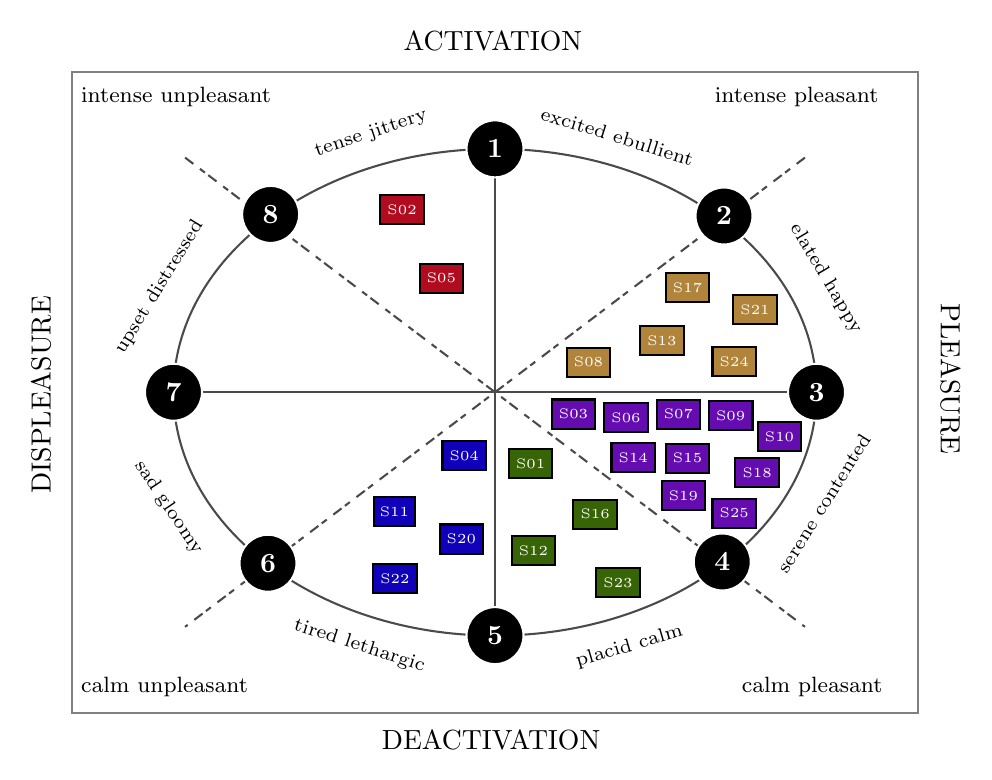
\begin{tikzpicture}[x=0.75pt,y=0.75pt,yscale=-1,xscale=1]
%uncomment if require: \path (0,389); %set diagram left start at 0, and has height of 389

%Flowchart: Or [id:dp3592995680476845] 
\draw  [color={rgb, 255:red, 74; green, 74; blue, 74 }  ,draw opacity=1 ] (182.64,181.1) .. controls (182.64,116.34) and (252,63.84) .. (337.55,63.84) .. controls (423.11,63.84) and (492.46,116.34) .. (492.46,181.1) .. controls (492.46,245.86) and (423.11,298.36) .. (337.55,298.36) .. controls (252,298.36) and (182.64,245.86) .. (182.64,181.1) -- cycle ; \draw  [color={rgb, 255:red, 74; green, 74; blue, 74 }  ,draw opacity=1 ] (182.64,181.1) -- (492.46,181.1) ; \draw  [color={rgb, 255:red, 74; green, 74; blue, 74 }  ,draw opacity=1 ] (337.55,63.84) -- (337.55,298.36) ;
%Straight Lines [id:da30798451784186187] 
\draw [color={rgb, 255:red, 74; green, 74; blue, 74 }  ,draw opacity=1 ] [dash pattern={on 3.75pt off 3pt on 2.25pt off 1.5pt}]  (188.22,68.06) -- (486.88,294.14) ;
%Straight Lines [id:da7804870395610348] 
\draw [color={rgb, 255:red, 74; green, 74; blue, 74 }  ,draw opacity=1 ] [dash pattern={on 3.75pt off 3pt on 2.25pt off 1.5pt}]  (486.88,68.06) -- (188.22,294.14) ;
%Shape: Rectangle [id:dp23344423808181314] 
\draw  [color={rgb, 255:red, 128; green, 128; blue, 128 }  ,draw opacity=1 ] (133.68,26.77) -- (541.42,26.77) -- (541.42,335.43) -- (133.68,335.43) -- cycle ;

% Text Node
\draw  [color={rgb, 255:red, 0; green, 0; blue, 0 }  ,draw opacity=1 ][fill={rgb, 255:red, 176; green, 11; blue, 31 }  ,fill opacity=1 ]  (282.29,86.22) -- (303.29,86.22) -- (303.29,100.22) -- (282.29,100.22) -- cycle  ;
\draw (292.79,93.22) node  [font=\tiny,color={rgb, 255:red, 255; green, 255; blue, 255 }  ,opacity=1 ] [align=left] {S02};
% Text Node
\draw  [color={rgb, 255:red, 0; green, 0; blue, 0 }  ,draw opacity=1 ][fill={rgb, 255:red, 17; green, 0; blue, 185 }  ,fill opacity=1 ]  (279.09,231.64) -- (299.09,231.64) -- (299.09,245.64) -- (279.09,245.64) -- cycle  ;
\draw (289.09,238.64) node  [font=\tiny,color={rgb, 255:red, 255; green, 255; blue, 255 }  ,opacity=1 ] [align=left] {S11};
% Text Node
\draw  [color={rgb, 255:red, 0; green, 0; blue, 0 }  ,draw opacity=1 ][fill={rgb, 255:red, 100; green, 12; blue, 176 }  ,fill opacity=1 ]  (364.87,184.61) -- (385.87,184.61) -- (385.87,198.61) -- (364.87,198.61) -- cycle  ;
\draw (375.37,191.61) node  [font=\tiny,color={rgb, 255:red, 255; green, 255; blue, 255 }  ,opacity=1 ] [align=left] {S03};
% Text Node
\draw  [color={rgb, 255:red, 0; green, 0; blue, 0 }  ,draw opacity=1 ][fill={rgb, 255:red, 176; green, 132; blue, 58 }  ,fill opacity=1 ]  (407.45,149.33) -- (428.45,149.33) -- (428.45,163.33) -- (407.45,163.33) -- cycle  ;
\draw (417.95,156.33) node  [font=\tiny,color={rgb, 255:red, 255; green, 255; blue, 255 }  ,opacity=1 ] [align=left] {S13};
% Text Node
\draw  [color={rgb, 255:red, 0; green, 0; blue, 0 }  ,draw opacity=1 ][fill={rgb, 255:red, 100; green, 12; blue, 176 }  ,fill opacity=1 ]  (440.62,185.49) -- (461.62,185.49) -- (461.62,199.49) -- (440.62,199.49) -- cycle  ;
\draw (451.12,192.49) node  [font=\tiny,color={rgb, 255:red, 255; green, 255; blue, 255 }  ,opacity=1 ] [align=left] {S09};
% Text Node
\draw  [color={rgb, 255:red, 0; green, 0; blue, 0 }  ,draw opacity=1 ][fill={rgb, 255:red, 55; green, 100; blue, 4 }  ,fill opacity=1 ]  (344.22,208.42) -- (365.22,208.42) -- (365.22,222.42) -- (344.22,222.42) -- cycle  ;
\draw (354.72,215.42) node  [font=\tiny,color={rgb, 255:red, 255; green, 255; blue, 255 }  ,opacity=1 ] [align=left] {S01};
% Text Node
\draw  [color={rgb, 255:red, 0; green, 0; blue, 0 }  ,draw opacity=1 ][fill={rgb, 255:red, 176; green, 11; blue, 31 }  ,fill opacity=1 ]  (301.25,119.14) -- (322.25,119.14) -- (322.25,133.14) -- (301.25,133.14) -- cycle  ;
\draw (311.75,126.14) node  [font=\tiny,color={rgb, 255:red, 255; green, 255; blue, 255 }  ,opacity=1 ] [align=left] {S05};
% Text Node
\draw  [color={rgb, 255:red, 0; green, 0; blue, 0 }  ,draw opacity=1 ][fill={rgb, 255:red, 17; green, 0; blue, 185 }  ,fill opacity=1 ]  (312.26,204.61) -- (333.26,204.61) -- (333.26,218.61) -- (312.26,218.61) -- cycle  ;
\draw (322.76,211.61) node  [font=\tiny,color={rgb, 255:red, 255; green, 255; blue, 255 }  ,opacity=1 ] [align=left] {S04};
% Text Node
\draw  [color={rgb, 255:red, 0; green, 0; blue, 0 }  ,draw opacity=1 ][fill={rgb, 255:red, 100; green, 12; blue, 176 }  ,fill opacity=1 ]  (419.83,205.83) -- (440.83,205.83) -- (440.83,219.83) -- (419.83,219.83) -- cycle  ;
\draw (430.33,212.83) node  [font=\tiny,color={rgb, 255:red, 255; green, 255; blue, 255 }  ,opacity=1 ] [align=left] {S15};
% Text Node
\draw  [color={rgb, 255:red, 0; green, 0; blue, 0 }  ,draw opacity=1 ][fill={rgb, 255:red, 100; green, 12; blue, 176 }  ,fill opacity=1 ]  (390.18,186.39) -- (411.18,186.39) -- (411.18,200.39) -- (390.18,200.39) -- cycle  ;
\draw (400.68,193.39) node  [font=\tiny,color={rgb, 255:red, 255; green, 255; blue, 255 }  ,opacity=1 ] [align=left] {S06};
% Text Node
\draw  [color={rgb, 255:red, 0; green, 0; blue, 0 }  ,draw opacity=1 ][fill={rgb, 255:red, 176; green, 132; blue, 58 }  ,fill opacity=1 ]  (372.1,159.61) -- (393.1,159.61) -- (393.1,173.61) -- (372.1,173.61) -- cycle  ;
\draw (382.6,166.61) node  [font=\tiny,color={rgb, 255:red, 255; green, 255; blue, 255 }  ,opacity=1 ] [align=left] {S08};
% Text Node
\draw  [color={rgb, 255:red, 0; green, 0; blue, 0 }  ,draw opacity=1 ][fill={rgb, 255:red, 100; green, 12; blue, 176 }  ,fill opacity=1 ]  (464.11,195.49) -- (485.11,195.49) -- (485.11,209.49) -- (464.11,209.49) -- cycle  ;
\draw (474.61,202.49) node  [font=\tiny,color={rgb, 255:red, 255; green, 255; blue, 255 }  ,opacity=1 ] [align=left] {S10};
% Text Node
\draw  [color={rgb, 255:red, 0; green, 0; blue, 0 }  ,draw opacity=1 ][fill={rgb, 255:red, 100; green, 12; blue, 176 }  ,fill opacity=1 ]  (393.68,205.71) -- (414.68,205.71) -- (414.68,219.71) -- (393.68,219.71) -- cycle  ;
\draw (404.18,212.71) node  [font=\tiny,color={rgb, 255:red, 255; green, 255; blue, 255 }  ,opacity=1 ] [align=left] {S14};
% Text Node
\draw  [color={rgb, 255:red, 0; green, 0; blue, 0 }  ,draw opacity=1 ][fill={rgb, 255:red, 55; green, 100; blue, 4 }  ,fill opacity=1 ]  (345.53,250.28) -- (366.53,250.28) -- (366.53,264.28) -- (345.53,264.28) -- cycle  ;
\draw (356.03,257.28) node  [font=\tiny,color={rgb, 255:red, 255; green, 255; blue, 255 }  ,opacity=1 ] [align=left] {S12};
% Text Node
\draw  [color={rgb, 255:red, 0; green, 0; blue, 0 }  ,draw opacity=1 ][fill={rgb, 255:red, 100; green, 12; blue, 176 }  ,fill opacity=1 ]  (415.44,184.66) -- (436.44,184.66) -- (436.44,198.66) -- (415.44,198.66) -- cycle  ;
\draw (425.94,191.66) node  [font=\tiny,color={rgb, 255:red, 255; green, 255; blue, 255 }  ,opacity=1 ] [align=left] {S07};
% Text Node
\draw  [color={rgb, 255:red, 255; green, 255; blue, 255 }  ,draw opacity=1 ][fill={rgb, 255:red, 0; green, 0; blue, 0 }  ,fill opacity=1 ]  (337.55, 63.84) circle [x radius= 13.73, y radius= 13.73]   ;
\draw (337.55,63.84) node  [font=\normalsize,color={rgb, 255:red, 255; green, 255; blue, 255 }  ,opacity=1 ] [align=left] {\textbf{1}};
% Text Node
\draw  [color={rgb, 255:red, 255; green, 255; blue, 255 }  ,draw opacity=1 ][fill={rgb, 255:red, 0; green, 0; blue, 0 }  ,fill opacity=1 ]  (447.88, 96.18) circle [x radius= 13.73, y radius= 13.73]   ;
\draw (447.88,96.18) node  [font=\normalsize,color={rgb, 255:red, 255; green, 255; blue, 255 }  ,opacity=1 ] [align=left] {\textbf{2}};
% Text Node
\draw  [color={rgb, 255:red, 255; green, 255; blue, 255 }  ,draw opacity=1 ][fill={rgb, 255:red, 0; green, 0; blue, 0 }  ,fill opacity=1 ]  (492.46, 181.1) circle [x radius= 13.73, y radius= 13.73]   ;
\draw (492.46,181.1) node  [font=\normalsize,color={rgb, 255:red, 255; green, 255; blue, 255 }  ,opacity=1 ] [align=left] {\textbf{3}};
% Text Node
\draw  [color={rgb, 255:red, 255; green, 255; blue, 255 }  ,draw opacity=1 ][fill={rgb, 255:red, 0; green, 0; blue, 0 }  ,fill opacity=1 ]  (447.05, 262.88) circle [x radius= 13.73, y radius= 13.73]   ;
\draw (447.05,262.88) node  [font=\normalsize,color={rgb, 255:red, 255; green, 255; blue, 255 }  ,opacity=1 ] [align=left] {\textbf{4}};
% Text Node
\draw  [color={rgb, 255:red, 255; green, 255; blue, 255 }  ,draw opacity=1 ][fill={rgb, 255:red, 0; green, 0; blue, 0 }  ,fill opacity=1 ]  (337.55, 298.36) circle [x radius= 13.73, y radius= 13.73]   ;
\draw (337.55,298.36) node  [font=\normalsize,color={rgb, 255:red, 255; green, 255; blue, 255 }  ,opacity=1 ] [align=left] {\textbf{5}};
% Text Node
\draw  [color={rgb, 255:red, 255; green, 255; blue, 255 }  ,draw opacity=1 ][fill={rgb, 255:red, 0; green, 0; blue, 0 }  ,fill opacity=1 ]  (228.16, 263.49) circle [x radius= 13.73, y radius= 13.73]   ;
\draw (228.16,263.49) node  [font=\normalsize,color={rgb, 255:red, 255; green, 255; blue, 255 }  ,opacity=1 ] [align=left] {\textbf{6}};
% Text Node
\draw  [color={rgb, 255:red, 255; green, 255; blue, 255 }  ,draw opacity=1 ][fill={rgb, 255:red, 0; green, 0; blue, 0 }  ,fill opacity=1 ]  (182.64, 181.1) circle [x radius= 13.73, y radius= 13.73]   ;
\draw (182.64,181.1) node  [font=\normalsize,color={rgb, 255:red, 255; green, 255; blue, 255 }  ,opacity=1 ] [align=left] {\textbf{7}};
% Text Node
\draw  [color={rgb, 255:red, 255; green, 255; blue, 255 }  ,draw opacity=1 ][fill={rgb, 255:red, 0; green, 0; blue, 0 }  ,fill opacity=1 ]  (229.45, 95.43) circle [x radius= 13.73, y radius= 13.73]   ;
\draw (229.45,95.43) node  [font=\normalsize,color={rgb, 255:red, 255; green, 255; blue, 255 }  ,opacity=1 ] [align=left] {\textbf{8}};
% Text Node
\draw (112.89,231.39) node [anchor=north west][inner sep=0.75pt]  [rotate=-270] [align=left] {DISPLEASURE};
% Text Node
\draw (292.08,5.96) node [anchor=north west][inner sep=0.75pt]   [align=left] {ACTIVATION};
% Text Node
\draw (281.58,342.71) node [anchor=north west][inner sep=0.75pt]   [align=left] {DEACTIVATION};
% Text Node
\draw (562.94,136.89) node [anchor=north west][inner sep=0.75pt]  [rotate=-90] [align=left] {PLEASURE};
% Text Node
\draw (150.9,160.23) node [anchor=north west][inner sep=0.75pt]  [font=\scriptsize,rotate=-301.49] [align=left] {upset distressed};
% Text Node
\draw (247.79,60.45) node [anchor=north west][inner sep=0.75pt]  [font=\scriptsize,rotate=-341.6] [align=left] {tense jittery};
% Text Node
\draw (359.94,41.46) node [anchor=north west][inner sep=0.75pt]  [font=\scriptsize,rotate=-17.34] [align=left] {excited ebullient};
% Text Node
\draw (485.75,96.5) node [anchor=north west][inner sep=0.75pt]  [font=\scriptsize,rotate=-59.2] [align=left] {elated happy};
% Text Node
\draw (470.66,265.95) node [anchor=north west][inner sep=0.75pt]  [font=\scriptsize,rotate=-301.93] [align=left] {serene contented};
% Text Node
\draw (373.68,306.2) node [anchor=north west][inner sep=0.75pt]  [font=\scriptsize,rotate=-343.65] [align=left] {placid calm};
% Text Node
\draw (241.21,287.33) node [anchor=north west][inner sep=0.75pt]  [font=\scriptsize,rotate=-18.04] [align=left] {tired lethargic};
% Text Node
\draw (169.56,210.51) node [anchor=north west][inner sep=0.75pt]  [font=\scriptsize,rotate=-56.13] [align=left] {sad gloomy};
% Text Node
\draw (455,317) node [anchor=north west][inner sep=0.75pt]  [font=\footnotesize] [align=left] {calm pleasant};
% Text Node
\draw (136.67,317) node [anchor=north west][inner sep=0.75pt]  [font=\footnotesize] [align=left] {calm unpleasant};
% Text Node
\draw (136.67,32.78) node [anchor=north west][inner sep=0.75pt]  [font=\footnotesize] [align=left] {intense unpleasant};
% Text Node
\draw (442,32.78) node [anchor=north west][inner sep=0.75pt]  [font=\footnotesize] [align=left] {intense pleasant};
% Text Node
\draw  [color={rgb, 255:red, 0; green, 0; blue, 0 }  ,draw opacity=1 ][fill={rgb, 255:red, 55; green, 100; blue, 4 }  ,fill opacity=1 ]  (375.33,232.83) -- (396.33,232.83) -- (396.33,246.83) -- (375.33,246.83) -- cycle  ;
\draw (385.83,239.83) node  [font=\tiny,color={rgb, 255:red, 255; green, 255; blue, 255 }  ,opacity=1 ] [align=left] {S16};
% Text Node
\draw  [color={rgb, 255:red, 0; green, 0; blue, 0 }  ,draw opacity=1 ][fill={rgb, 255:red, 176; green, 132; blue, 58 }  ,fill opacity=1 ]  (419.83,123.83) -- (440.83,123.83) -- (440.83,137.83) -- (419.83,137.83) -- cycle  ;
\draw (430.33,130.83) node  [font=\tiny,color={rgb, 255:red, 255; green, 255; blue, 255 }  ,opacity=1 ] [align=left] {S17};
% Text Node
\draw  [color={rgb, 255:red, 0; green, 0; blue, 0 }  ,draw opacity=1 ][fill={rgb, 255:red, 100; green, 12; blue, 176 }  ,fill opacity=1 ]  (453.33,212.83) -- (474.33,212.83) -- (474.33,226.83) -- (453.33,226.83) -- cycle  ;
\draw (463.83,219.83) node  [font=\tiny,color={rgb, 255:red, 255; green, 255; blue, 255 }  ,opacity=1 ] [align=left] {S18};
% Text Node
\draw  [color={rgb, 255:red, 0; green, 0; blue, 0 }  ,draw opacity=1 ][fill={rgb, 255:red, 100; green, 12; blue, 176 }  ,fill opacity=1 ]  (417.83,223.83) -- (438.83,223.83) -- (438.83,237.83) -- (417.83,237.83) -- cycle  ;
\draw (428.33,230.83) node  [font=\tiny,color={rgb, 255:red, 255; green, 255; blue, 255 }  ,opacity=1 ] [align=left] {S19};
% Text Node
\draw  [color={rgb, 255:red, 0; green, 0; blue, 0 }  ,draw opacity=1 ][fill={rgb, 255:red, 17; green, 0; blue, 185 }  ,fill opacity=1 ]  (310.83,244.83) -- (331.83,244.83) -- (331.83,258.83) -- (310.83,258.83) -- cycle  ;
\draw (321.33,251.83) node  [font=\tiny,color={rgb, 255:red, 255; green, 255; blue, 255 }  ,opacity=1 ] [align=left] {S20};
% Text Node
\draw  [color={rgb, 255:red, 0; green, 0; blue, 0 }  ,draw opacity=1 ][fill={rgb, 255:red, 176; green, 132; blue, 58 }  ,fill opacity=1 ]  (452.33,134.33) -- (473.33,134.33) -- (473.33,148.33) -- (452.33,148.33) -- cycle  ;
\draw (462.83,141.33) node  [font=\tiny,color={rgb, 255:red, 255; green, 255; blue, 255 }  ,opacity=1 ] [align=left] {S21};
% Text Node
\draw  [color={rgb, 255:red, 0; green, 0; blue, 0 }  ,draw opacity=1 ][fill={rgb, 255:red, 17; green, 0; blue, 185 }  ,fill opacity=1 ]  (278.83,263.83) -- (299.83,263.83) -- (299.83,277.83) -- (278.83,277.83) -- cycle  ;
\draw (289.33,270.83) node  [font=\tiny,color={rgb, 255:red, 255; green, 255; blue, 255 }  ,opacity=1 ] [align=left] {S22};
% Text Node
\draw  [color={rgb, 255:red, 0; green, 0; blue, 0 }  ,draw opacity=1 ][fill={rgb, 255:red, 55; green, 100; blue, 4 }  ,fill opacity=1 ]  (386.33,265.83) -- (407.33,265.83) -- (407.33,279.83) -- (386.33,279.83) -- cycle  ;
\draw (396.83,272.83) node  [font=\tiny,color={rgb, 255:red, 255; green, 255; blue, 255 }  ,opacity=1 ] [align=left] {S23};
% Text Node
\draw  [color={rgb, 255:red, 0; green, 0; blue, 0 }  ,draw opacity=1 ][fill={rgb, 255:red, 176; green, 132; blue, 58 }  ,fill opacity=1 ]  (442.33,159.33) -- (463.33,159.33) -- (463.33,173.33) -- (442.33,173.33) -- cycle  ;
\draw (452.83,166.33) node  [font=\tiny,color={rgb, 255:red, 255; green, 255; blue, 255 }  ,opacity=1 ] [align=left] {S24};
% Text Node
\draw  [color={rgb, 255:red, 0; green, 0; blue, 0 }  ,draw opacity=1 ][fill={rgb, 255:red, 100; green, 12; blue, 176 }  ,fill opacity=1 ]  (442.33,232.33) -- (463.33,232.33) -- (463.33,246.33) -- (442.33,246.33) -- cycle  ;
\draw (452.83,239.33) node  [font=\tiny,color={rgb, 255:red, 255; green, 255; blue, 255 }  ,opacity=1 ] [align=left] {S25};


\end{tikzpicture}

    \fonte{Author.}
\end{figure}


\cleardoublepage

%######################################################
\subsection{Experiment 3}
\label{ssec_experiments:Experiment3}
%######################################################
Aqui o terceiro experimento...

\begin{figure}[!htb]
    \centering
    \caption{Emocards terceiro experimento - ERtext}
    \label{fig:Emocards4_alt}
    

\tikzset{every picture/.style={line width=0.75pt}} %set default line width to 0.75pt        

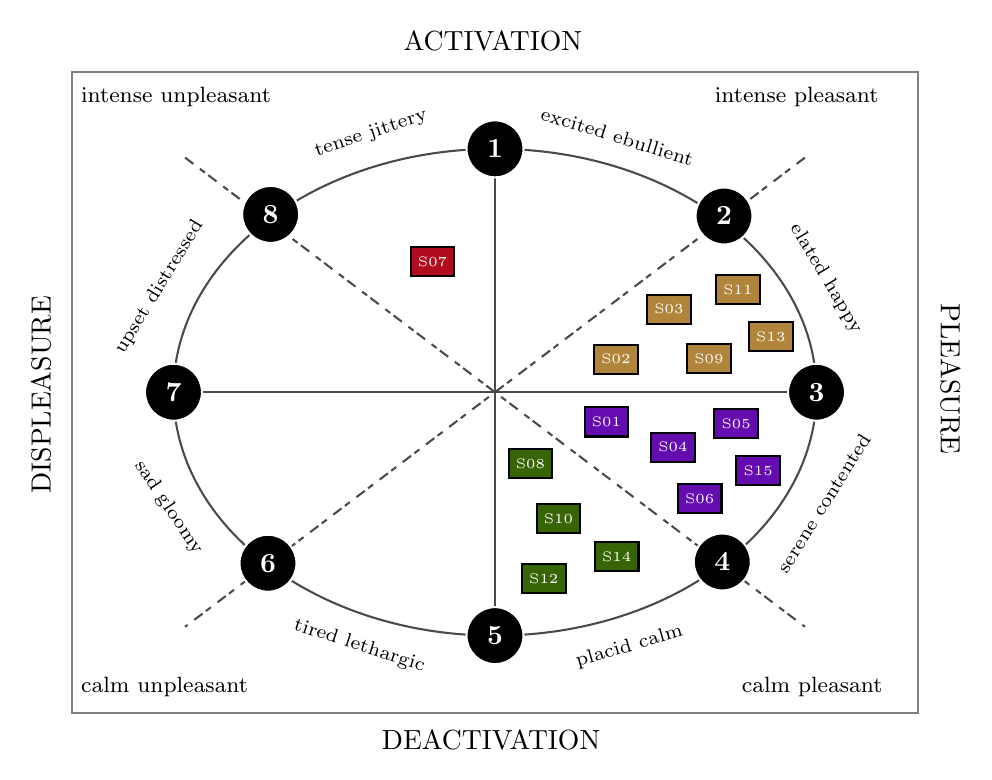
\begin{tikzpicture}[x=0.75pt,y=0.75pt,yscale=-1,xscale=1]
%uncomment if require: \path (0,389); %set diagram left start at 0, and has height of 389

%Flowchart: Or [id:dp3592995680476845] 
\draw  [color={rgb, 255:red, 74; green, 74; blue, 74 }  ,draw opacity=1 ] (182.64,181.1) .. controls (182.64,116.34) and (252,63.84) .. (337.55,63.84) .. controls (423.11,63.84) and (492.46,116.34) .. (492.46,181.1) .. controls (492.46,245.86) and (423.11,298.36) .. (337.55,298.36) .. controls (252,298.36) and (182.64,245.86) .. (182.64,181.1) -- cycle ; \draw  [color={rgb, 255:red, 74; green, 74; blue, 74 }  ,draw opacity=1 ] (182.64,181.1) -- (492.46,181.1) ; \draw  [color={rgb, 255:red, 74; green, 74; blue, 74 }  ,draw opacity=1 ] (337.55,63.84) -- (337.55,298.36) ;
%Straight Lines [id:da30798451784186187] 
\draw [color={rgb, 255:red, 74; green, 74; blue, 74 }  ,draw opacity=1 ] [dash pattern={on 3.75pt off 3pt on 2.25pt off 1.5pt}]  (188.22,68.06) -- (486.88,294.14) ;
%Straight Lines [id:da7804870395610348] 
\draw [color={rgb, 255:red, 74; green, 74; blue, 74 }  ,draw opacity=1 ] [dash pattern={on 3.75pt off 3pt on 2.25pt off 1.5pt}]  (486.88,68.06) -- (188.22,294.14) ;
%Shape: Rectangle [id:dp23344423808181314] 
\draw  [color={rgb, 255:red, 128; green, 128; blue, 128 }  ,draw opacity=1 ] (133.68,26.77) -- (541.42,26.77) -- (541.42,335.43) -- (133.68,335.43) -- cycle ;

% Text Node
\draw  [color={rgb, 255:red, 0; green, 0; blue, 0 }  ,draw opacity=1 ][fill={rgb, 255:red, 176; green, 132; blue, 58 }  ,fill opacity=1 ]  (385.29,158.22) -- (406.29,158.22) -- (406.29,172.22) -- (385.29,172.22) -- cycle  ;
\draw (395.79,165.22) node  [font=\tiny,color={rgb, 255:red, 255; green, 255; blue, 255 }  ,opacity=1 ] [align=left] {S02};
% Text Node
\draw  [color={rgb, 255:red, 0; green, 0; blue, 0 }  ,draw opacity=1 ][fill={rgb, 255:red, 176; green, 132; blue, 58 }  ,fill opacity=1 ]  (444.09,124.64) -- (465.09,124.64) -- (465.09,138.64) -- (444.09,138.64) -- cycle  ;
\draw (454.59,131.64) node  [font=\tiny,color={rgb, 255:red, 255; green, 255; blue, 255 }  ,opacity=1 ] [align=left] {S11};
% Text Node
\draw  [color={rgb, 255:red, 0; green, 0; blue, 0 }  ,draw opacity=1 ][fill={rgb, 255:red, 176; green, 132; blue, 58 }  ,fill opacity=1 ]  (410.87,134.11) -- (431.87,134.11) -- (431.87,148.11) -- (410.87,148.11) -- cycle  ;
\draw (421.37,141.11) node  [font=\tiny,color={rgb, 255:red, 255; green, 255; blue, 255 }  ,opacity=1 ] [align=left] {S03};
% Text Node
\draw  [color={rgb, 255:red, 0; green, 0; blue, 0 }  ,draw opacity=1 ][fill={rgb, 255:red, 176; green, 132; blue, 58 }  ,fill opacity=1 ]  (459.95,147.33) -- (480.95,147.33) -- (480.95,161.33) -- (459.95,161.33) -- cycle  ;
\draw (470.45,154.33) node  [font=\tiny,color={rgb, 255:red, 255; green, 255; blue, 255 }  ,opacity=1 ] [align=left] {S13};
% Text Node
\draw  [color={rgb, 255:red, 0; green, 0; blue, 0 }  ,draw opacity=1 ][fill={rgb, 255:red, 176; green, 132; blue, 58 }  ,fill opacity=1 ]  (430.12,157.99) -- (451.12,157.99) -- (451.12,171.99) -- (430.12,171.99) -- cycle  ;
\draw (440.62,164.99) node  [font=\tiny,color={rgb, 255:red, 255; green, 255; blue, 255 }  ,opacity=1 ] [align=left] {S09};
% Text Node
\draw  [color={rgb, 255:red, 0; green, 0; blue, 0 }  ,draw opacity=1 ][fill={rgb, 255:red, 100; green, 12; blue, 176 }  ,fill opacity=1 ]  (380.72,188.42) -- (401.72,188.42) -- (401.72,202.42) -- (380.72,202.42) -- cycle  ;
\draw (391.22,195.42) node  [font=\tiny,color={rgb, 255:red, 255; green, 255; blue, 255 }  ,opacity=1 ] [align=left] {S01};
% Text Node
\draw  [color={rgb, 255:red, 0; green, 0; blue, 0 }  ,draw opacity=1 ][fill={rgb, 255:red, 100; green, 12; blue, 176 }  ,fill opacity=1 ]  (443.25,189.14) -- (464.25,189.14) -- (464.25,203.14) -- (443.25,203.14) -- cycle  ;
\draw (453.75,196.14) node  [font=\tiny,color={rgb, 255:red, 255; green, 255; blue, 255 }  ,opacity=1 ] [align=left] {S05};
% Text Node
\draw  [color={rgb, 255:red, 0; green, 0; blue, 0 }  ,draw opacity=1 ][fill={rgb, 255:red, 100; green, 12; blue, 176 }  ,fill opacity=1 ]  (412.76,200.61) -- (433.76,200.61) -- (433.76,214.61) -- (412.76,214.61) -- cycle  ;
\draw (423.26,207.61) node  [font=\tiny,color={rgb, 255:red, 255; green, 255; blue, 255 }  ,opacity=1 ] [align=left] {S04};
% Text Node
\draw  [color={rgb, 255:red, 0; green, 0; blue, 0 }  ,draw opacity=1 ][fill={rgb, 255:red, 100; green, 12; blue, 176 }  ,fill opacity=1 ]  (453.83,211.83) -- (474.83,211.83) -- (474.83,225.83) -- (453.83,225.83) -- cycle  ;
\draw (464.33,218.83) node  [font=\tiny,color={rgb, 255:red, 255; green, 255; blue, 255 }  ,opacity=1 ] [align=left] {S15};
% Text Node
\draw  [color={rgb, 255:red, 0; green, 0; blue, 0 }  ,draw opacity=1 ][fill={rgb, 255:red, 100; green, 12; blue, 176 }  ,fill opacity=1 ]  (425.68,225.39) -- (446.68,225.39) -- (446.68,239.39) -- (425.68,239.39) -- cycle  ;
\draw (436.18,232.39) node  [font=\tiny,color={rgb, 255:red, 255; green, 255; blue, 255 }  ,opacity=1 ] [align=left] {S06};
% Text Node
\draw  [color={rgb, 255:red, 0; green, 0; blue, 0 }  ,draw opacity=1 ][fill={rgb, 255:red, 55; green, 100; blue, 4 }  ,fill opacity=1 ]  (344.1,208.52) -- (365.1,208.52) -- (365.1,222.52) -- (344.1,222.52) -- cycle  ;
\draw (354.6,215.52) node  [font=\tiny,color={rgb, 255:red, 255; green, 255; blue, 255 }  ,opacity=1 ] [align=left] {S08};
% Text Node
\draw  [color={rgb, 255:red, 0; green, 0; blue, 0 }  ,draw opacity=1 ][fill={rgb, 255:red, 55; green, 100; blue, 4 }  ,fill opacity=1 ]  (357.61,234.99) -- (378.61,234.99) -- (378.61,248.99) -- (357.61,248.99) -- cycle  ;
\draw (368.11,241.99) node  [font=\tiny,color={rgb, 255:red, 255; green, 255; blue, 255 }  ,opacity=1 ] [align=left] {S10};
% Text Node
\draw  [color={rgb, 255:red, 0; green, 0; blue, 0 }  ,draw opacity=1 ][fill={rgb, 255:red, 55; green, 100; blue, 4 }  ,fill opacity=1 ]  (385.68,253.21) -- (406.68,253.21) -- (406.68,267.21) -- (385.68,267.21) -- cycle  ;
\draw (396.18,260.21) node  [font=\tiny,color={rgb, 255:red, 255; green, 255; blue, 255 }  ,opacity=1 ] [align=left] {S14};
% Text Node
\draw  [color={rgb, 255:red, 0; green, 0; blue, 0 }  ,draw opacity=1 ][fill={rgb, 255:red, 55; green, 100; blue, 4 }  ,fill opacity=1 ]  (350.53,263.78) -- (371.53,263.78) -- (371.53,277.78) -- (350.53,277.78) -- cycle  ;
\draw (361.03,270.78) node  [font=\tiny,color={rgb, 255:red, 255; green, 255; blue, 255 }  ,opacity=1 ] [align=left] {S12};
% Text Node
\draw  [color={rgb, 255:red, 0; green, 0; blue, 0 }  ,draw opacity=1 ][fill={rgb, 255:red, 176; green, 11; blue, 31 }  ,fill opacity=1 ]  (296.94,111.16) -- (317.94,111.16) -- (317.94,125.16) -- (296.94,125.16) -- cycle  ;
\draw (307.44,118.16) node  [font=\tiny,color={rgb, 255:red, 255; green, 255; blue, 255 }  ,opacity=1 ] [align=left] {S07};
% Text Node
\draw  [color={rgb, 255:red, 255; green, 255; blue, 255 }  ,draw opacity=1 ][fill={rgb, 255:red, 0; green, 0; blue, 0 }  ,fill opacity=1 ]  (337.55, 63.84) circle [x radius= 13.73, y radius= 13.73]   ;
\draw (337.55,63.84) node  [font=\normalsize,color={rgb, 255:red, 255; green, 255; blue, 255 }  ,opacity=1 ] [align=left] {\textbf{1}};
% Text Node
\draw  [color={rgb, 255:red, 255; green, 255; blue, 255 }  ,draw opacity=1 ][fill={rgb, 255:red, 0; green, 0; blue, 0 }  ,fill opacity=1 ]  (447.88, 96.18) circle [x radius= 13.73, y radius= 13.73]   ;
\draw (447.88,96.18) node  [font=\normalsize,color={rgb, 255:red, 255; green, 255; blue, 255 }  ,opacity=1 ] [align=left] {\textbf{2}};
% Text Node
\draw  [color={rgb, 255:red, 255; green, 255; blue, 255 }  ,draw opacity=1 ][fill={rgb, 255:red, 0; green, 0; blue, 0 }  ,fill opacity=1 ]  (492.46, 181.1) circle [x radius= 13.73, y radius= 13.73]   ;
\draw (492.46,181.1) node  [font=\normalsize,color={rgb, 255:red, 255; green, 255; blue, 255 }  ,opacity=1 ] [align=left] {\textbf{3}};
% Text Node
\draw  [color={rgb, 255:red, 255; green, 255; blue, 255 }  ,draw opacity=1 ][fill={rgb, 255:red, 0; green, 0; blue, 0 }  ,fill opacity=1 ]  (447.05, 262.88) circle [x radius= 13.73, y radius= 13.73]   ;
\draw (447.05,262.88) node  [font=\normalsize,color={rgb, 255:red, 255; green, 255; blue, 255 }  ,opacity=1 ] [align=left] {\textbf{4}};
% Text Node
\draw  [color={rgb, 255:red, 255; green, 255; blue, 255 }  ,draw opacity=1 ][fill={rgb, 255:red, 0; green, 0; blue, 0 }  ,fill opacity=1 ]  (337.55, 298.36) circle [x radius= 13.73, y radius= 13.73]   ;
\draw (337.55,298.36) node  [font=\normalsize,color={rgb, 255:red, 255; green, 255; blue, 255 }  ,opacity=1 ] [align=left] {\textbf{5}};
% Text Node
\draw  [color={rgb, 255:red, 255; green, 255; blue, 255 }  ,draw opacity=1 ][fill={rgb, 255:red, 0; green, 0; blue, 0 }  ,fill opacity=1 ]  (228.16, 263.49) circle [x radius= 13.73, y radius= 13.73]   ;
\draw (228.16,263.49) node  [font=\normalsize,color={rgb, 255:red, 255; green, 255; blue, 255 }  ,opacity=1 ] [align=left] {\textbf{6}};
% Text Node
\draw  [color={rgb, 255:red, 255; green, 255; blue, 255 }  ,draw opacity=1 ][fill={rgb, 255:red, 0; green, 0; blue, 0 }  ,fill opacity=1 ]  (182.64, 181.1) circle [x radius= 13.73, y radius= 13.73]   ;
\draw (182.64,181.1) node  [font=\normalsize,color={rgb, 255:red, 255; green, 255; blue, 255 }  ,opacity=1 ] [align=left] {\textbf{7}};
% Text Node
\draw  [color={rgb, 255:red, 255; green, 255; blue, 255 }  ,draw opacity=1 ][fill={rgb, 255:red, 0; green, 0; blue, 0 }  ,fill opacity=1 ]  (229.45, 95.43) circle [x radius= 13.73, y radius= 13.73]   ;
\draw (229.45,95.43) node  [font=\normalsize,color={rgb, 255:red, 255; green, 255; blue, 255 }  ,opacity=1 ] [align=left] {\textbf{8}};
% Text Node
\draw (112.89,231.39) node [anchor=north west][inner sep=0.75pt]  [rotate=-270] [align=left] {DISPLEASURE};
% Text Node
\draw (292.08,5.96) node [anchor=north west][inner sep=0.75pt]   [align=left] {ACTIVATION};
% Text Node
\draw (281.58,342.71) node [anchor=north west][inner sep=0.75pt]   [align=left] {DEACTIVATION};
% Text Node
\draw (562.94,136.89) node [anchor=north west][inner sep=0.75pt]  [rotate=-90] [align=left] {PLEASURE};
% Text Node
\draw (150.9,160.23) node [anchor=north west][inner sep=0.75pt]  [font=\scriptsize,rotate=-301.49] [align=left] {upset distressed};
% Text Node
\draw (247.79,60.45) node [anchor=north west][inner sep=0.75pt]  [font=\scriptsize,rotate=-341.6] [align=left] {tense jittery};
% Text Node
\draw (359.94,41.46) node [anchor=north west][inner sep=0.75pt]  [font=\scriptsize,rotate=-17.34] [align=left] {excited ebullient};
% Text Node
\draw (485.75,96.5) node [anchor=north west][inner sep=0.75pt]  [font=\scriptsize,rotate=-59.2] [align=left] {elated happy};
% Text Node
\draw (470.66,265.95) node [anchor=north west][inner sep=0.75pt]  [font=\scriptsize,rotate=-301.93] [align=left] {serene contented};
% Text Node
\draw (373.68,306.2) node [anchor=north west][inner sep=0.75pt]  [font=\scriptsize,rotate=-343.65] [align=left] {placid calm};
% Text Node
\draw (241.21,287.33) node [anchor=north west][inner sep=0.75pt]  [font=\scriptsize,rotate=-18.04] [align=left] {tired lethargic};
% Text Node
\draw (169.56,210.51) node [anchor=north west][inner sep=0.75pt]  [font=\scriptsize,rotate=-56.13] [align=left] {sad gloomy};
% Text Node
\draw (455,317) node [anchor=north west][inner sep=0.75pt]  [font=\footnotesize] [align=left] {calm pleasant};
% Text Node
\draw (136.67,317) node [anchor=north west][inner sep=0.75pt]  [font=\footnotesize] [align=left] {calm unpleasant};
% Text Node
\draw (136.67,32.78) node [anchor=north west][inner sep=0.75pt]  [font=\footnotesize] [align=left] {intense unpleasant};
% Text Node
\draw (442,32.78) node [anchor=north west][inner sep=0.75pt]  [font=\footnotesize] [align=left] {intense pleasant};


\end{tikzpicture}

    \fonte{Author.}
\end{figure}

\begin{figure}[!htb]
    \centering
    \caption{Emocards terceiro experimento - brModelo}
    \label{fig:Emocards3_alt}
    \tikzset{every picture/.style={line width=0.75pt}} %set default line width to 0.75pt        

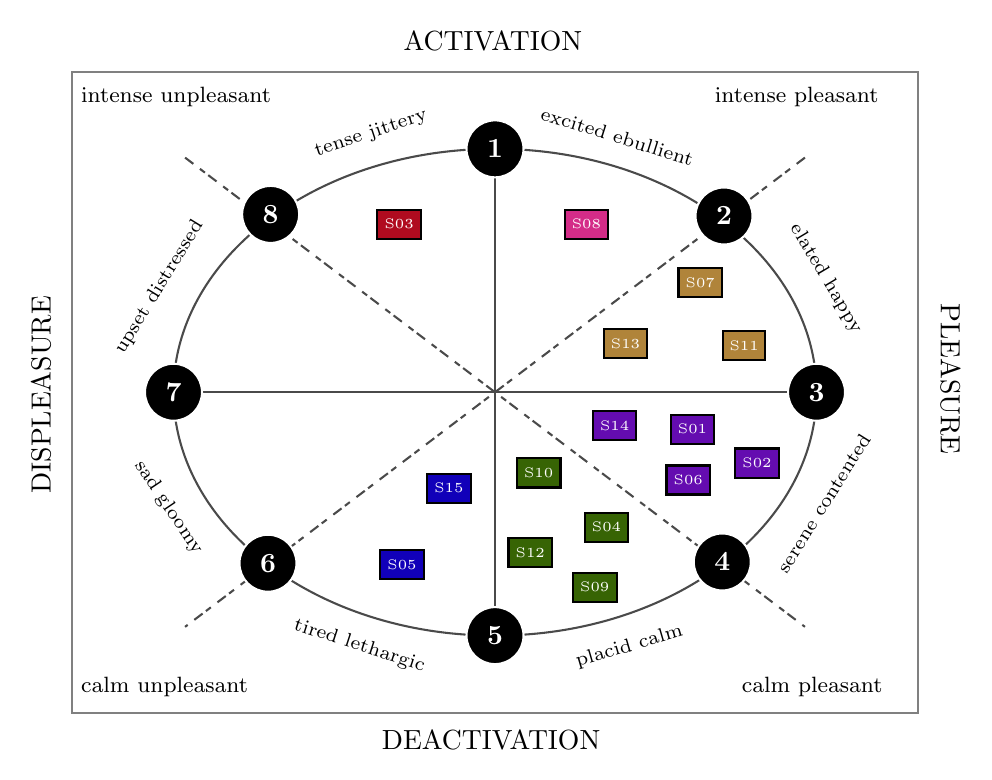
\begin{tikzpicture}[x=0.75pt,y=0.75pt,yscale=-1,xscale=1]
%uncomment if require: \path (0,389); %set diagram left start at 0, and has height of 389

%Flowchart: Or [id:dp3592995680476845] 
\draw  [color={rgb, 255:red, 74; green, 74; blue, 74 }  ,draw opacity=1 ] (182.64,181.1) .. controls (182.64,116.34) and (252,63.84) .. (337.55,63.84) .. controls (423.11,63.84) and (492.46,116.34) .. (492.46,181.1) .. controls (492.46,245.86) and (423.11,298.36) .. (337.55,298.36) .. controls (252,298.36) and (182.64,245.86) .. (182.64,181.1) -- cycle ; \draw  [color={rgb, 255:red, 74; green, 74; blue, 74 }  ,draw opacity=1 ] (182.64,181.1) -- (492.46,181.1) ; \draw  [color={rgb, 255:red, 74; green, 74; blue, 74 }  ,draw opacity=1 ] (337.55,63.84) -- (337.55,298.36) ;
%Straight Lines [id:da30798451784186187] 
\draw [color={rgb, 255:red, 74; green, 74; blue, 74 }  ,draw opacity=1 ] [dash pattern={on 3.75pt off 3pt on 2.25pt off 1.5pt}]  (188.22,68.06) -- (486.88,294.14) ;
%Straight Lines [id:da7804870395610348] 
\draw [color={rgb, 255:red, 74; green, 74; blue, 74 }  ,draw opacity=1 ] [dash pattern={on 3.75pt off 3pt on 2.25pt off 1.5pt}]  (486.88,68.06) -- (188.22,294.14) ;
%Shape: Rectangle [id:dp23344423808181314] 
\draw  [color={rgb, 255:red, 128; green, 128; blue, 128 }  ,draw opacity=1 ] (133.68,26.77) -- (541.42,26.77) -- (541.42,335.43) -- (133.68,335.43) -- cycle ;

% Text Node
\draw  [color={rgb, 255:red, 0; green, 0; blue, 0 }  ,draw opacity=1 ][fill={rgb, 255:red, 100; green, 12; blue, 176 }  ,fill opacity=1 ]  (453.29,208.22) -- (474.29,208.22) -- (474.29,222.22) -- (453.29,222.22) -- cycle  ;
\draw (463.79,215.22) node  [font=\tiny,color={rgb, 255:red, 255; green, 255; blue, 255 }  ,opacity=1 ] [align=left] {S02};
% Text Node
\draw  [color={rgb, 255:red, 0; green, 0; blue, 0 }  ,draw opacity=1 ][fill={rgb, 255:red, 176; green, 132; blue, 58 }  ,fill opacity=1 ]  (447.59,151.64) -- (467.59,151.64) -- (467.59,165.64) -- (447.59,165.64) -- cycle  ;
\draw (457.59,158.64) node  [font=\tiny,color={rgb, 255:red, 255; green, 255; blue, 255 }  ,opacity=1 ] [align=left] {S11};
% Text Node
\draw  [color={rgb, 255:red, 0; green, 0; blue, 0 }  ,draw opacity=1 ][fill={rgb, 255:red, 176; green, 11; blue, 31 }  ,fill opacity=1 ]  (280.87,93.11) -- (301.87,93.11) -- (301.87,107.11) -- (280.87,107.11) -- cycle  ;
\draw (291.37,100.11) node  [font=\tiny,color={rgb, 255:red, 255; green, 255; blue, 255 }  ,opacity=1 ] [align=left] {S03};
% Text Node
\draw  [color={rgb, 255:red, 0; green, 0; blue, 0 }  ,draw opacity=1 ][fill={rgb, 255:red, 176; green, 132; blue, 58 }  ,fill opacity=1 ]  (389.95,150.83) -- (410.95,150.83) -- (410.95,164.83) -- (389.95,164.83) -- cycle  ;
\draw (400.45,157.83) node  [font=\tiny,color={rgb, 255:red, 255; green, 255; blue, 255 }  ,opacity=1 ] [align=left] {S13};
% Text Node
\draw  [color={rgb, 255:red, 0; green, 0; blue, 0 }  ,draw opacity=1 ][fill={rgb, 255:red, 55; green, 100; blue, 4 }  ,fill opacity=1 ]  (375.12,267.99) -- (396.12,267.99) -- (396.12,281.99) -- (375.12,281.99) -- cycle  ;
\draw (385.62,274.99) node  [font=\tiny,color={rgb, 255:red, 255; green, 255; blue, 255 }  ,opacity=1 ] [align=left] {S09};
% Text Node
\draw  [color={rgb, 255:red, 0; green, 0; blue, 0 }  ,draw opacity=1 ][fill={rgb, 255:red, 100; green, 12; blue, 176 }  ,fill opacity=1 ]  (422.22,191.92) -- (443.22,191.92) -- (443.22,205.92) -- (422.22,205.92) -- cycle  ;
\draw (432.72,198.92) node  [font=\tiny,color={rgb, 255:red, 255; green, 255; blue, 255 }  ,opacity=1 ] [align=left] {S01};
% Text Node
\draw  [color={rgb, 255:red, 0; green, 0; blue, 0 }  ,draw opacity=1 ][fill={rgb, 255:red, 17; green, 0; blue, 185 }  ,fill opacity=1 ]  (282.25,257.14) -- (303.25,257.14) -- (303.25,271.14) -- (282.25,271.14) -- cycle  ;
\draw (292.75,264.14) node  [font=\tiny,color={rgb, 255:red, 255; green, 255; blue, 255 }  ,opacity=1 ] [align=left] {S05};
% Text Node
\draw  [color={rgb, 255:red, 0; green, 0; blue, 0 }  ,draw opacity=1 ][fill={rgb, 255:red, 55; green, 100; blue, 4 }  ,fill opacity=1 ]  (380.76,239.11) -- (401.76,239.11) -- (401.76,253.11) -- (380.76,253.11) -- cycle  ;
\draw (391.26,246.11) node  [font=\tiny,color={rgb, 255:red, 255; green, 255; blue, 255 }  ,opacity=1 ] [align=left] {S04};
% Text Node
\draw  [color={rgb, 255:red, 0; green, 0; blue, 0 }  ,draw opacity=1 ][fill={rgb, 255:red, 17; green, 0; blue, 185 }  ,fill opacity=1 ]  (304.83,220.33) -- (325.83,220.33) -- (325.83,234.33) -- (304.83,234.33) -- cycle  ;
\draw (315.33,227.33) node  [font=\tiny,color={rgb, 255:red, 255; green, 255; blue, 255 }  ,opacity=1 ] [align=left] {S15};
% Text Node
\draw  [color={rgb, 255:red, 0; green, 0; blue, 0 }  ,draw opacity=1 ][fill={rgb, 255:red, 100; green, 12; blue, 176 }  ,fill opacity=1 ]  (420.18,216.39) -- (441.18,216.39) -- (441.18,230.39) -- (420.18,230.39) -- cycle  ;
\draw (430.68,223.39) node  [font=\tiny,color={rgb, 255:red, 255; green, 255; blue, 255 }  ,opacity=1 ] [align=left] {S06};
% Text Node
\draw  [color={rgb, 255:red, 0; green, 0; blue, 0 }  ,draw opacity=1 ][fill={rgb, 255:red, 212; green, 44; blue, 136 }  ,fill opacity=1 ]  (371.1,93.11) -- (392.1,93.11) -- (392.1,107.11) -- (371.1,107.11) -- cycle  ;
\draw (381.6,100.11) node  [font=\tiny,color={rgb, 255:red, 255; green, 255; blue, 255 }  ,opacity=1 ] [align=left] {S08};
% Text Node
\draw  [color={rgb, 255:red, 0; green, 0; blue, 0 }  ,draw opacity=1 ][fill={rgb, 255:red, 55; green, 100; blue, 4 }  ,fill opacity=1 ]  (348.11,212.99) -- (369.11,212.99) -- (369.11,226.99) -- (348.11,226.99) -- cycle  ;
\draw (358.61,219.99) node  [font=\tiny,color={rgb, 255:red, 255; green, 255; blue, 255 }  ,opacity=1 ] [align=left] {S10};
% Text Node
\draw  [color={rgb, 255:red, 0; green, 0; blue, 0 }  ,draw opacity=1 ][fill={rgb, 255:red, 100; green, 12; blue, 176 }  ,fill opacity=1 ]  (384.68,190.21) -- (405.68,190.21) -- (405.68,204.21) -- (384.68,204.21) -- cycle  ;
\draw (395.18,197.21) node  [font=\tiny,color={rgb, 255:red, 255; green, 255; blue, 255 }  ,opacity=1 ] [align=left] {S14};
% Text Node
\draw  [color={rgb, 255:red, 0; green, 0; blue, 0 }  ,draw opacity=1 ][fill={rgb, 255:red, 55; green, 100; blue, 4 }  ,fill opacity=1 ]  (344.03,251.28) -- (365.03,251.28) -- (365.03,265.28) -- (344.03,265.28) -- cycle  ;
\draw (354.53,258.28) node  [font=\tiny,color={rgb, 255:red, 255; green, 255; blue, 255 }  ,opacity=1 ] [align=left] {S12};
% Text Node
\draw  [color={rgb, 255:red, 0; green, 0; blue, 0 }  ,draw opacity=1 ][fill={rgb, 255:red, 176; green, 132; blue, 58 }  ,fill opacity=1 ]  (425.94,121.16) -- (446.94,121.16) -- (446.94,135.16) -- (425.94,135.16) -- cycle  ;
\draw (436.44,128.16) node  [font=\tiny,color={rgb, 255:red, 255; green, 255; blue, 255 }  ,opacity=1 ] [align=left] {S07};
% Text Node
\draw  [color={rgb, 255:red, 255; green, 255; blue, 255 }  ,draw opacity=1 ][fill={rgb, 255:red, 0; green, 0; blue, 0 }  ,fill opacity=1 ]  (337.55, 63.84) circle [x radius= 13.73, y radius= 13.73]   ;
\draw (337.55,63.84) node  [font=\normalsize,color={rgb, 255:red, 255; green, 255; blue, 255 }  ,opacity=1 ] [align=left] {\textbf{1}};
% Text Node
\draw  [color={rgb, 255:red, 255; green, 255; blue, 255 }  ,draw opacity=1 ][fill={rgb, 255:red, 0; green, 0; blue, 0 }  ,fill opacity=1 ]  (447.88, 96.18) circle [x radius= 13.73, y radius= 13.73]   ;
\draw (447.88,96.18) node  [font=\normalsize,color={rgb, 255:red, 255; green, 255; blue, 255 }  ,opacity=1 ] [align=left] {\textbf{2}};
% Text Node
\draw  [color={rgb, 255:red, 255; green, 255; blue, 255 }  ,draw opacity=1 ][fill={rgb, 255:red, 0; green, 0; blue, 0 }  ,fill opacity=1 ]  (492.46, 181.1) circle [x radius= 13.73, y radius= 13.73]   ;
\draw (492.46,181.1) node  [font=\normalsize,color={rgb, 255:red, 255; green, 255; blue, 255 }  ,opacity=1 ] [align=left] {\textbf{3}};
% Text Node
\draw  [color={rgb, 255:red, 255; green, 255; blue, 255 }  ,draw opacity=1 ][fill={rgb, 255:red, 0; green, 0; blue, 0 }  ,fill opacity=1 ]  (447.05, 262.88) circle [x radius= 13.73, y radius= 13.73]   ;
\draw (447.05,262.88) node  [font=\normalsize,color={rgb, 255:red, 255; green, 255; blue, 255 }  ,opacity=1 ] [align=left] {\textbf{4}};
% Text Node
\draw  [color={rgb, 255:red, 255; green, 255; blue, 255 }  ,draw opacity=1 ][fill={rgb, 255:red, 0; green, 0; blue, 0 }  ,fill opacity=1 ]  (337.55, 298.36) circle [x radius= 13.73, y radius= 13.73]   ;
\draw (337.55,298.36) node  [font=\normalsize,color={rgb, 255:red, 255; green, 255; blue, 255 }  ,opacity=1 ] [align=left] {\textbf{5}};
% Text Node
\draw  [color={rgb, 255:red, 255; green, 255; blue, 255 }  ,draw opacity=1 ][fill={rgb, 255:red, 0; green, 0; blue, 0 }  ,fill opacity=1 ]  (228.16, 263.49) circle [x radius= 13.73, y radius= 13.73]   ;
\draw (228.16,263.49) node  [font=\normalsize,color={rgb, 255:red, 255; green, 255; blue, 255 }  ,opacity=1 ] [align=left] {\textbf{6}};
% Text Node
\draw  [color={rgb, 255:red, 255; green, 255; blue, 255 }  ,draw opacity=1 ][fill={rgb, 255:red, 0; green, 0; blue, 0 }  ,fill opacity=1 ]  (182.64, 181.1) circle [x radius= 13.73, y radius= 13.73]   ;
\draw (182.64,181.1) node  [font=\normalsize,color={rgb, 255:red, 255; green, 255; blue, 255 }  ,opacity=1 ] [align=left] {\textbf{7}};
% Text Node
\draw  [color={rgb, 255:red, 255; green, 255; blue, 255 }  ,draw opacity=1 ][fill={rgb, 255:red, 0; green, 0; blue, 0 }  ,fill opacity=1 ]  (229.45, 95.43) circle [x radius= 13.73, y radius= 13.73]   ;
\draw (229.45,95.43) node  [font=\normalsize,color={rgb, 255:red, 255; green, 255; blue, 255 }  ,opacity=1 ] [align=left] {\textbf{8}};
% Text Node
\draw (112.89,231.39) node [anchor=north west][inner sep=0.75pt]  [rotate=-270] [align=left] {DISPLEASURE};
% Text Node
\draw (292.08,5.96) node [anchor=north west][inner sep=0.75pt]   [align=left] {ACTIVATION};
% Text Node
\draw (281.58,342.71) node [anchor=north west][inner sep=0.75pt]   [align=left] {DEACTIVATION};
% Text Node
\draw (562.94,136.89) node [anchor=north west][inner sep=0.75pt]  [rotate=-90] [align=left] {PLEASURE};
% Text Node
\draw (150.9,160.23) node [anchor=north west][inner sep=0.75pt]  [font=\scriptsize,rotate=-301.49] [align=left] {upset distressed};
% Text Node
\draw (247.79,60.45) node [anchor=north west][inner sep=0.75pt]  [font=\scriptsize,rotate=-341.6] [align=left] {tense jittery};
% Text Node
\draw (359.94,41.46) node [anchor=north west][inner sep=0.75pt]  [font=\scriptsize,rotate=-17.34] [align=left] {excited ebullient};
% Text Node
\draw (485.75,96.5) node [anchor=north west][inner sep=0.75pt]  [font=\scriptsize,rotate=-59.2] [align=left] {elated happy};
% Text Node
\draw (470.66,265.95) node [anchor=north west][inner sep=0.75pt]  [font=\scriptsize,rotate=-301.93] [align=left] {serene contented};
% Text Node
\draw (373.68,306.2) node [anchor=north west][inner sep=0.75pt]  [font=\scriptsize,rotate=-343.65] [align=left] {placid calm};
% Text Node
\draw (241.21,287.33) node [anchor=north west][inner sep=0.75pt]  [font=\scriptsize,rotate=-18.04] [align=left] {tired lethargic};
% Text Node
\draw (169.56,210.51) node [anchor=north west][inner sep=0.75pt]  [font=\scriptsize,rotate=-56.13] [align=left] {sad gloomy};
% Text Node
\draw (455,317) node [anchor=north west][inner sep=0.75pt]  [font=\footnotesize] [align=left] {calm pleasant};
% Text Node
\draw (136.67,317) node [anchor=north west][inner sep=0.75pt]  [font=\footnotesize] [align=left] {calm unpleasant};
% Text Node
\draw (136.67,32.78) node [anchor=north west][inner sep=0.75pt]  [font=\footnotesize] [align=left] {intense unpleasant};
% Text Node
\draw (442,32.78) node [anchor=north west][inner sep=0.75pt]  [font=\footnotesize] [align=left] {intense pleasant};

\end{tikzpicture}

    \fonte{Author.}
\end{figure}

\begin{figure}[!htb]
    \centering
    \caption{Avaliação dos Modelos produzidos - Ambas as tools}
    \label{fig:ToolModelsEval}
    \pgfplotsset{testbar/.style={
        xbar stacked,
        legend cell align=left,
        legend style={
            legend columns=8,
            font=\scriptsize,
            at={(xticklabel cs:1.0)},
            anchor=north east,
            draw=none,
            nodes={scale=1}
            },
        width=10cm,
        axis y line*= none, 
        axis x line*= bottom,
        xmajorgrids = false,
        xmin=0,xmax=15,
        ytick = data,
        yticklabels = {
            {\scriptsize Conceptual Model-ERtext},
            {\scriptsize Conceptual Model-brModelo},
            {\scriptsize Logical Model-ERtext},
            {\scriptsize Logical Model-brModelo},
            {\scriptsize Physical Model-ERtext},
            {\scriptsize Physical Model-brModelo}
        },
        tick align = outside, 
        xtick pos = left,
        xticklabel style = {font=\scriptsize},
        bar width=3.5mm, 
        y=6.5mm,
        enlarge y limits={abs=0.450},% 0.5 + 0.5*(y - bar width)/y [TeX.sx #47995]
        nodes near coords,
        nodes near coords align=center,%Move values in bar
        every node near coord/.append style={
            black,
            font=\scriptsize,
            text opacity=1,
            fill=white,
            fill opacity=0.5,
            outer sep=\pgflinewidth
        }
    }}
    \begin{tikzpicture}
    \begin{axis}[testbar] 
    \addplot[pattern color=red,pattern=north east lines] coordinates
        {(0,6)(0,5)(0,4)(0,3)(0,2)(0,1)};
    \addplot[pattern color=teal,pattern=vertical lines] coordinates
        {(0,6)(0,5)(0,4)(0,3)(0,2)(0,1)};
    \addplot[pattern color=gray, pattern=grid] coordinates
        {(2,6)(0,5)(2,4)(2,3)(0,2)(3,1)};
    \addplot[pattern color=magenta, pattern=north west lines] coordinates
        {(1,6)(0,5)(2,4)(1,3)(3,2)(3,1)};
    \addplot[pattern color=blue, pattern=horizontal lines] coordinates
        {(5,6)(4,5)(4,4)(7,3)(3,2)(4,1)};
    \addplot[pattern color=green, pattern=crosshatch dots] coordinates
        {(7,6)(11,5)(7,4)(5,3)(9,2)(5,1)};
    \legend{1-Strongly Bad, 2, 3, 4, 5, 6-Strongly Good}
    \end{axis}
    \end{tikzpicture}
    \fonte{Author.}
\end{figure}

% \begin{figure}[!htb]
%     \centering
%     \caption{SUS terceiro experimento - ERtext}
%     \label{fig:SUSERtext}
%     \pgfplotsset{testbar/.style={
        xbar stacked,
        legend cell align=left,
        legend style={
            legend columns=8,
            font=\scriptsize,
            at={(xticklabel cs:1.0)},
            anchor=north east,
            draw=none,
            nodes={scale=1}
            },
        width=10cm,
        axis y line*= none, 
        axis x line*= bottom,
        xmajorgrids = false,
        xmin=0,xmax=15,
        ytick = data,
        yticklabels = {
            {\scriptsize SUS1},
            {\scriptsize SUS2},
            {\scriptsize SUS3},
            {\scriptsize SUS4},
            {\scriptsize SUS5},
            {\scriptsize SUS6}, 
            {\scriptsize SUS7},
            {\scriptsize SUS8},
            {\scriptsize SUS9},
            {\scriptsize SUS10}
        },
        tick align = outside, 
        xtick pos = left,
        xticklabel style = {font=\scriptsize},
        bar width=3.5mm, 
        y=6.5mm,
        enlarge y limits={abs=0.450},% 0.5 + 0.5*(y - bar width)/y [TeX.sx #47995]
        nodes near coords,
        nodes near coords align=center,%Move values in bar
        every node near coord/.append style={
            black,
            font=\scriptsize,
            text opacity=1,
            fill=white,
            fill opacity=0.5,
            outer sep=\pgflinewidth
        }
    }}
    \begin{tikzpicture}
    \begin{axis}[testbar] 
    \addplot[pattern color=red,pattern=north east lines] coordinates
       {(0,10)(6,9)(0,8)(4,7)(0,6)(10,5)(0,4)(9,3)(0,2)(5,1)};
    \addplot[pattern color=teal,pattern=vertical lines] coordinates
        {(0,10)(3,9)(0,8)(4,7)(0,6)(3,5)(0,4)(4,3)(1,2)(1,1)};
    \addplot[pattern color=magenta, pattern=north west lines] coordinates
        {(1,10)(5,9)(2,8)(4,7)(3,6)(1,5)(2,4)(2,3)(1,2)(5,1)};
    \addplot[pattern color=blue, pattern=horizontal lines] coordinates
        {(7,10)(1,9)(5,8)(3,7)(5,6)(1,5)(7,4)(0,3)(7,2)(3,1)};
    \addplot[pattern color=green, pattern=crosshatch dots] coordinates
        {(7,10)(0,9)(8,8)(0,7)(7,6)(0,5)(6,4)(0,3)(6,2)(1,1)};
    \legend{1-Strongly Disagree, 2, 3, 4, 5-Strongly Agree}
    \end{axis}
    \end{tikzpicture}
    

%     \fonte{Author.}
% \end{figure}

% \begin{figure}[!htb]
%     \centering
%     \caption{SUS terceiro experimento - brModelo}
%     \label{fig:SUSbrModelo}
%     \pgfplotsset{testbar/.style={
        xbar stacked,
        legend cell align=left,
        legend style={
            legend columns=8,
            font=\scriptsize,
            at={(xticklabel cs:1.0)},
            anchor=north east,
            draw=none,
            nodes={scale=1}
            },
        width=10cm,
        axis y line*= none, 
        axis x line*= bottom,
        xmajorgrids = false,
        xmin=0,xmax=15,
        ytick = data,
        yticklabels = {
            {\scriptsize SUS1},
            {\scriptsize SUS2},
            {\scriptsize SUS3},
            {\scriptsize SUS4},
            {\scriptsize SUS5},
            {\scriptsize SUS6}, 
            {\scriptsize SUS7},
            {\scriptsize SUS8},
            {\scriptsize SUS9},
            {\scriptsize SUS10}
        },
        tick align = outside, 
        xtick pos = left,
        xticklabel style = {font=\scriptsize},
        bar width=3.5mm, 
        y=6.5mm,
        enlarge y limits={abs=0.450},% 0.5 + 0.5*(y - bar width)/y [TeX.sx #47995]
        nodes near coords,
        nodes near coords align=center,%Move values in bar
        every node near coord/.append style={
            black,
            font=\scriptsize,
            text opacity=1,
            fill=white,
            fill opacity=0.5,
            outer sep=\pgflinewidth
        }
    }}
    \begin{tikzpicture}
    \begin{axis}[testbar] 
    \addplot[pattern color=red,pattern=north east lines] coordinates
        {(0,10)(8,9)(0,8)(5,7)(0,6)(6,5)(0,4)(9,3)(0,2)(3,1)};
    \addplot[pattern color=teal,pattern=vertical lines] coordinates
        {(0,10)(6,9)(1,8)(5,7)(0,6)(5,5)(1,4)(5,3)(1,2)(7,1)};
    \addplot[pattern color=magenta, pattern=north west lines] coordinates
        {(5,10)(0,9)(2,8)(2,7)(5,6)(2,5)(1,4)(0,3)(3,2)(3,1)};
    \addplot[pattern color=blue, pattern=horizontal lines] coordinates
        {(3,10)(1,9)(4,8)(3,7)(6,6)(1,5)(9,4)(1,3)(6,2)(2,1)};
    \addplot[pattern color=green, pattern=crosshatch dots] coordinates
        {(7,10)(0,9)(8,8)(0,7)(4,6)(1,5)(4,4)(0,3)(5,2)(0,1)};
    \legend{1-Strongly Disagree, 2, 3, 4, 5-Strongly Agree}
    \end{axis}
    \end{tikzpicture}

%     \fonte{Author.}
% \end{figure}

% \begin{figure}[!htb]
%     \centering
%     \caption{SUS terceiro experimento - Ambas as tools}
%     \label{fig:SUS_tools}
%     \pgfplotsset{testbar/.style={
        xbar stacked,
        legend cell align=left,
        legend style={
            legend columns=8,
            font=\scriptsize,
            at={(xticklabel cs:1.0)},
            anchor=north east,
            draw=none,
            nodes={scale=1}
            },
        width=10cm,
        axis y line*= none, 
        axis x line*= bottom,
        xmajorgrids = false,
        xmin=0,xmax=15,
        ytick = data,
        yticklabels = {
            {\scriptsize SUS1-ERtext},
            {\scriptsize SUS1-brModelo},
            {\scriptsize SUS2-ERtext},
            {\scriptsize SUS2-brModelo},
            {\scriptsize SUS3-ERtext},
            {\scriptsize SUS3-brModelo},
            {\scriptsize SUS4-ERtext},
            {\scriptsize SUS4-brModelo},
            {\scriptsize SUS5-ERtext},
            {\scriptsize SUS5-brModelo},
            {\scriptsize SUS6-ERtext},
            {\scriptsize SUS6-brModelo},
            {\scriptsize SUS7-ERtext},
            {\scriptsize SUS7-brModelo},
            {\scriptsize SUS8-ERtext},
            {\scriptsize SUS8-brModelo},
            {\scriptsize SUS9-ERtext},
            {\scriptsize SUS9-brModelo},
            {\scriptsize SUS10-ERtext},
            {\scriptsize SUS10-brModelo}
        },
        tick align = outside, 
        xtick pos = left,
        xticklabel style = {font=\scriptsize},
        bar width=3.5mm, 
        y=6.5mm,
        enlarge y limits={abs=0.450},% 0.5 + 0.5*(y - bar width)/y [TeX.sx #47995]
        nodes near coords,
        nodes near coords align=center,%Move values in bar
        every node near coord/.append style={
            black,
            font=\scriptsize,
            text opacity=1,
            fill=white,
            fill opacity=0.5,
            outer sep=\pgflinewidth
        }
    }}
    \begin{tikzpicture}
    \begin{axis}[testbar] 
    \addplot[pattern color=red,pattern=north east lines] coordinates
        {(0,20)(0,19)(8,18)(6,17)(0,16)(0,15)(5,14)(4,13)(0,12)(0,11)(6,10)(10,9)(0,8)(0,7)(9,6)(9,5)(0,4)(0,3)(3,2)(5,1)};
    \addplot[pattern color=teal,pattern=vertical lines] coordinates
       {(0,20)(0,19)(6,18)(3,17)(1,16)(0,15)(5,14)(4,13)(0,12)(0,11)(5,10)(3,9)(1,8)(0,7)(5,6)(4,5)(1,4)(1,3)(7,2)(1,1)}; 
    \addplot[pattern color=magenta, pattern=north west lines] coordinates
        {(5,20)(1,19)(0,18)(5,17)(2,16)(2,15)(2,14)(4,13)(5,12)(3,11)(2,10)(1,9)(1,8)(2,7(0,6))(2,5)(3,4)(1,3)(3,2)(5,1)};
    \addplot[pattern color=blue, pattern=horizontal lines] coordinates
        {(3,20)(7,19)(1,18)(1,17)(4,16)(5,15)(3,14)(3,13)(6,12)(5,11)(1,10)(1,9)(9,8)(7,7)(1,6)(0,5)(6,4)(7,3)(2,2)(3,1)};
    \addplot[pattern color=green, pattern=crosshatch dots] coordinates
        {(7,20)(7,19)(0,18)(0,17)(8,16)(8,15)(0,14)(0,13)(4,12)(7,11)(1,10)(0,9)(4,8)(6,7)(0,6)(0,5)(5,4)(6,3)(0,2)(1,1)};
    \legend{1-Strongly Disagree, 2, 3, 4, 5-Strongly Agree}
    \end{axis}
    \end{tikzpicture}
    
    
    
    
   
    

%     \fonte{Author.}
% \end{figure}

\begin{figure}[!htb]
    \centering
    \caption{BoxPlot SUS terceiro experimento - Ambas as tools}
    \label{fig:BoxPlotSUS_tools}
    \begin{filecontents*}{data5.csv}
37.5,50,72.5,72.5,75,75,75,80,80,82.5,85,85,87.5,95,100
50,60,67.5,67.5,67.5,70,70,75,80,90,92.5,92.5,97.5,97.5,100
\end{filecontents*}

\makeatletter
\pgfplotsset{
    boxplot/hide outliers/.code={
        \def\pgfplotsplothandlerboxplot@outlier{}%
    }
}
\makeatother

\begin{tikzpicture}
    \pgfplotstableread[col sep=comma]{data5.csv}\csvdata
    % Boxplot groups columns, but we want rows
    \pgfplotstabletranspose\datatransposed{\csvdata} 
    \begin{axis}[
         boxplot/draw direction=y,
        xtick={1, 2},
        ylabel={\scriptsize Percentage (\%)},
        xticklabels={{\scriptsize Graphical Treatment}, {\scriptsize Textual Treatment}},
        height=7cm,
        width=10cm,
        % boxplot/draw direction = y,
        % axis x line* = bottom,
        % axis y line = left,
        % enlarge y limits,
        ymajorgrids,
        % xtick = {1, 2},
        % xticklabel style = {align=center, font=\small},
        % xticklabels = {Graphical Treatment, Textual Treatment},
        % ylabel = {Percentage (\%)},
        ytick = {40, 50, 60, 70, 80, 90},
        yticklabel style = {font=\scriptsize}
    ]
        \foreach \n in {1,...,2} {
            \addplot+[boxplot, fill, fill opacity=0.4, draw=black] table[y index=\n] {\datatransposed};
        }
    \end{axis}
\end{tikzpicture}



    \fonte{Author.}
\end{figure}

\begin{figure}[!htb]
    \centering
    \caption{Grouped Bar Chart SUS terceiro experimento - Ambas as tools}
    \label{fig:GroupedBarSUS_tools}
    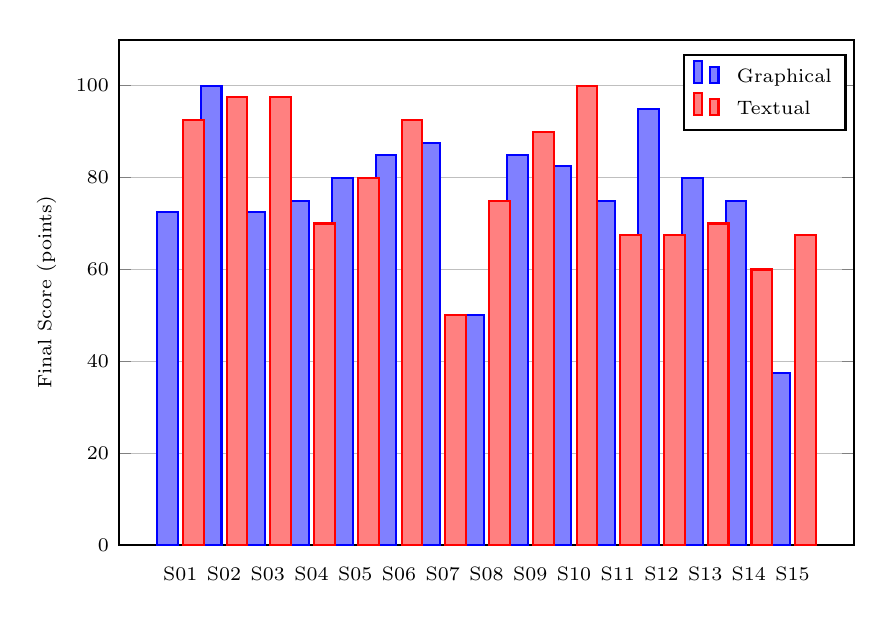
\begin{tikzpicture}
    \begin{axis}[
        width  = 0.90\textwidth,
        height = 8cm,
        major x tick style = transparent,
        ybar=2.5*\pgflinewidth,
        bar width=7.5pt,
        ymajorgrids = true,
        ylabel = {Final Score (points)},
        symbolic x coords={
        S01, S02, S03, S04, S05, S06, S07, S08, S09, S10, S11, S12, S13, S14, S15
        },
        xtick = data,
        scaled y ticks = false,
        % enlarge x limits=0.20,
        ymin=0,
        label style={font=\scriptsize},
        tick label style={font=\scriptsize},
        legend cell align=left,
        legend style={
                at={(0.99,0.82)},
                anchor=south east,
                column sep=1ex,
                font = \scriptsize
        }
    ]
        \addplot[style={blue,fill=blue!50}]
            coordinates {
            (S01,72.5) (S02,100) (S03,72.5) (S04,75) (S05,80) (S06,85) (S07,87.5) (S08,50) (S09,85) (S10,82.5) (S11,75) (S12,95) (S13,80) (S14,75) (S15,37.5)
            };

        \addplot[style={red,fill=red!50}]
            coordinates {
            (S01,92.5) (S02,97.5) (S03,97.5) (S04,70) (S05,80) (S06,92.5) (S07,50) (S08,75) (S09,90) (S10,100) (S11,67.5) (S12,67.5) (S13,70) (S14,60) (S15,67.5)
            };
            
        \legend{Graphical,Textual}
    \end{axis}
\end{tikzpicture}
    \fonte{Author.}
\end{figure}

\rowcolors{1}{gray!15}{white}
\begin{table}[!htb]
    \caption{Measures of the SUS (System Usability Scale) in the third experiment.}
    \label{tab:ResultsSUS}
    \centering
    \scriptsize
    % \tiny
    \begin{tabular}{l|ccccc|ccccc}%{l|ccccc|ccccc}
    \bottomrule
    \rowcolor[HTML]{C0C0C0}
    \multicolumn{1}{l}{} &
    \multicolumn{1}{c|}{\textbf{Graphical Treatment}} &
    \multicolumn{1}{c}{\textbf{Textual Treatment}}
    \\ 
    \hline
    \rowcolor[HTML]{C0C0C0}
    \textbf{Measure} & \textbf{SUS Final Score} & \textbf{SUS Final Score}
    \\
    \hline
Maximum	&	100.00	&	100.00		\\
3\textdegree Quartile	&	85.00	&	92.50	\\
Average	&	76.83	&	78.50	\\
Median	&	80.00	&	75.00	\\
1\textdegree Quartile	&	73.75	&	67.50	\\
Minimum	&	37.50	&	50.00	\\
Variance	&	248.63	&	241.79	\\
SD	&	15.77	&	15.55	\\
    \toprule
\end{tabular}
\begin{tablenotes}
    \scriptsize
    \centering
    \item \textit{Legend: SD = Standard Deviation.}
\end{tablenotes}
\fonte{Author.}
\end{table}

- FAZER MAPEAMENTO ENTRE AVALIAÇÃO QUALITATIVA (SUJEITOS X RESPOSTAS) E EMOCARDS

- Um paragrafo para cada code e tentar contrapor 

- Trabalho futuro: Definir esquema de cores personalizada para os modelos criados

\cleardoublepage
%------------------------------------------------------------------------------
\section{Chapter Lessons}
\label{sec_experiments:lessons}
%------------------------------------------------------------------------------

This chapter presented a preliminary controlled experiment (Experiment 1) replication with a sample of 33 subjects evaluating ERtext, a proposed textual \ac{dsl} tool for \acp{db} conceptual modeling. 
We compared the ERtext with the brModelo, a graphical \ac{dsl} well-known in Software Engineering ER lectures. 
With the results obtained, it was possible to answer the experiment's four RQs, as well as the two associated hypotheses.
In this sense, we can say that we investigated three main aspects of our \ac{dsl}: effort, effectiveness, and quality in use.

From the analysis, it is possible to highlight the following aspects:

\item \textbf{Effort:} The computed average difference states that there are no differences between the approaches, \textit{i.e.}, one approach is not better than the other. 

\item \textbf{Effectiveness:} Through the statistical test we reject the null hypothesis that the approaches are equally effective. 
When comparing the box-plot graphs produced, it is possible to observe a slight advantage for the textual approach. 
In the first experiment (Experiment 1), the result was different since the tests indicated that there was no significant difference. 
We believe that the biggest reason for this event is that all participants in this replication are undergraduate students at the very beginning of the academy program, basically without any more previous experience with graphic modeling tools. 
In the first experiment, there were, in addition to these, master and doctoral students. 
We also do not discard possible influences caused by the fact that the experiment was conducted remotely in the pandemic context.

\item \textbf{Qualitative comparison between treatments:} We observed a certain balance between treatments, but with a positive evaluation for ERtext regarding the ``Productivity'' and ``Operability'' attributes.
Because it was the first time that the subjects had contact with our grammar, and also considering the first release of our DSL and the negative feedback also collected, we conclude that ERtext is on the rails for achieving better productivity indexes.

We also collected qualitative feedback from subjects. 
As a result, there are some improvements regarding the DSL design that need to be revised, in particular to the ternary relationships and self-relationships.
Since the continuity of DSL development is foreseen, the execution of a possible refactoring, and also the implementation of new ER builders, is a natural step for its software evolution.
From the preliminary experimental results, we conclude that there is feasibility and good perspectives for the motivating context, \textit{i.e.}, as a tool for teaching ER modeling with the differential of adopting a textual approach for conceptual \ac{db} modeling in classrooms instead of a graphical notation.

% Finalmente, nós esperamos complementar as lições deste capítulo em breve com a avaliação experimental que ainda será realizada.
Finally, we hope to supplement the lessons in this chapter shortly by carrying out the experimental evaluation yet.